% !TeX spellcheck = en_US
\documentclass[AIRstudentthesis%      style
              ,optCharter%            font
              ,optBlackHeadings%      black sections to reduce number of colored pages
              ,optBlackRefs%          black references to reduce number of colored pages
              %,optCMYK%              color model
              ,optBiber%              bibliography tool
              ,optBibstyleAlphabetic% bibliography style
              ,optCenterEquations%    alignment of equations
              ,optEnglish%            language
              %,optTikzExternalize%   compiles faster for large tikz images
              ]{AIRlatex}
%
% Load additional LaTeX packages - remove what you do not need
\usepackage{algorithm}%
\usepackage{algorithmicx}%
\usepackage{booktabs}%
%\usepackage{url}
\usepackage{amsmath}
\usepackage{graphicx}
\usepackage{subcaption}
\usepackage{listings}
\usepackage{xcolor}
\usepackage{array}
\usepackage{multirow}
\usepackage{bm}
\usepackage{caption}
\usepackage{colortbl}
\usepackage{bigstrut}
\usepackage{comment}
\usepackage[edges]{forest}
\usetikzlibrary{shadows.blur}
\usepackage{tabularx}
\usepackage{siunitx} % for S column type

% Define dark green and dark red
\definecolor{darkgreen}{RGB}{100,205,50}
\definecolor{darkred}{RGB}{220,20,60}

% Define JSON formatting
\definecolor{jsonorange}{RGB}{255,140,0}
\definecolor{jsonpurple}{RGB}{128,0,128}
\definecolor{jsonblue}{RGB}{0,0,255}
\definecolor{jsonstring}{RGB}{0,128,0}
\definecolor{anglebracketcolor}{RGB}{255,0,0}

\lstdefinelanguage{json}{
	basicstyle=\small\ttfamily,
	commentstyle=\color{gray},
	stringstyle=\color{jsonstring},
	numberstyle=\tiny\color{black},
	showstringspaces=false,
	breaklines=true,
	breakatwhitespace=true,
	columns=flexible,
	frame=lines,
	backgroundcolor=\color{gray!10},
	extendedchars=true,
	basewidth = {.15em},
	numbers=left, % display line numbers on the left
	moredelim=[is][\color{gray}]{*}{*},,
	moredelim=[is][\color{jsonpurple}]{<}{>},
	literate=
	*%{0}{{{\color{jsonpurple}0}}}{1}
	%{1}{{{\color{jsonpurple}1}}}{1}
	%{2}{{{\color{jsonpurple}2}}}{1}
	%{3}{{{\color{jsonpurple}3}}}{1}
	%{4}{{{\color{jsonpurple}4}}}{1}
	%{5}{{{\color{jsonpurple}5}}}{1}
	%{6}{{{\color{jsonpurple}6}}}{1}
	%{7}{{{\color{jsonpurple}7}}}{1}
	%{8}{{{\color{jsonpurple}8}}}{1}
	%{9}{{{\color{jsonpurple}9}}}{1}
	{:}{{{\color{jsonblue}{:}}}}{1}
	{,}{{{\color{jsonblue}{,}}}}{1}
	{\{}{{{\color{jsonblue}{\{}}}}{1}
	{\}}{{{\color{jsonblue}{\}}}}}{1}
	{[}{{{\color{jsonblue}{[}}}}{1}
	{]}{{{\color{jsonblue}{]}}}}{1},
}

%
% Set paths
\graphicspath{{figures/}}%
\addbibresource{source/literature.bib}%
%
% Define additional commands
\newcommand{\code}[1]{\texttt{#1}}%
\newcommand{\degree}[0]{^\circ}%
%
\begin{document}%
% Titlepage
% ---------
\frontmatter%
% Info: separate multiple supervisors by \newline
%\AIRstudentthesisTitlePageCustomDiplomarbeit{German Title}{English Title}{\AIRlangFieldOfStudyRoboticsCognitionIntelligence}{Martin Mustermann}{}{\AIRnamesProfKnoll}{Musterbetreuer, M.Sc.}{\AIRutilsDate{1}{1}{2020}}%
\AIRstudentthesisTitlePageCustomBachelorsThesis{Monokulare 3D-Wahrnehmung mit Hilfe von Infrastruktursensorik basierend auf Instanzsegmentierung}{Monocular Roadside 3D Perception based on Instance Segmentation}{\AIRlangFieldOfStudyRoboticsCognitionIntelligence}{Bach Ngoc Doan}{}{\AIRnamesProfKnoll}{Walter Zimmer, M.Sc.}{\AIRutilsDate{15}{2}{2024}}%
%\AIRstudentthesisTitlePageCustomSemesterThesis{German Title}{English Title}{\AIRlangFieldOfStudyRoboticsCognitionIntelligence}{Martin Mustermann}{}{\AIRnamesProfKnoll}{Musterbetreuer, M.Sc.}{\AIRutilsDate{1}{1}{2020}}%
%\AIRstudentthesisTitlePageCustomIDP{German Title}{English Title}{\AIRlangFieldOfStudyRoboticsCognitionIntelligence}{Martin Mustermann}{}{\AIRnamesProfKnoll}{Musterbetreuer, M.Sc.}{\AIRutilsDate{1}{1}{2020}}%
%\AIRstudentthesisTitlePageCustomMastersThesis{German Title}{Monocular Roadside 3D Perception based on Amodal Instance Segmentation}{\AIRlangFieldOfStudyRoboticsCognitionIntelligence}{Bach Ngoc Doan}{}{\AIRnamesProfKnoll}{Walter Zimmer, M.Sc.}{\AIRutilsDate{15}{2}{2024}}%
%
% Abstract
% --------
% In total max. 1 Page!
\AIRstudentthesisAbstract{%
%
% Abstract English:
\hl{TODO}
%
}{%
%
% Zusammenfassung Deutsch:
\hl{TODO}
%
}%
%
%
%
\AIRstudentthesisAcknowledgement{%
	
	I would like to express my sincere thanks to my thesis advisor, Walter Zimmer, for his guidance throughout the literature research process, his support in helping me understand the existing toolchain and his valuable feedback on my work.
	
}%
%
% Content
% -------
\AIRstudentthesisPrintTableOfContents%
\mainmatter%
% !TeX spellcheck = en_US
\chapter{Introduction}%

\section{AUTOTech.agil Project}

This thesis is a part of the project AUTOTech.agil, which is funded by the federal ministry of transport and digital infrastructure under the initiative “Digital Test Beds for Autonomous Driving”. The project is equipped with 7 sensor stations and 75 sensors along the A9-Highway, with a goal of providing solutions and recommendations to improve traffic safety, efficiency and comfort.

\hl{

- the Providentia++ project. The Federal Ministry has funded the project for Digital and Transport since 2017. Since 2020, it has been led by the Chair of Robotics, Artificial Intelligence, and Real-time Systems at the Technical University of Munich’s Department of Informatics.
- Initially, two measurement stations with cameras and Radio Detection and Ranging (Radar) sensors were installed on a test section of the A9 highway near Garching. The sensor data was used to identify vehicles using artificial intelligence and then fused. The resulting digital twin can be used by autonomous cars to make decisions based on events that could not be perceived solely by the vehicle’s onboard sensors.
- The second phase of the project started in 2020. Light Detection and Ranging (LiDAR) sensors were added to the existing perception methods. In addition, the test stretch was expanded into the residential area, which allows surveying intersections, traffic circles, bus stations, and other urban situations.

}


\section{Motivation}
\hl{TODO}

\section{Contributions}
\hl{TODO}
- Our contributions can be summarized as:
- The contributions of this work are summarized as follows:
- In summary, the main contributions of this work are:
- This work presents the following research contributions:

- Extend annotation. 

\section{Structure of the Thesis}
\hl{TODO}
%
% !TeX spellcheck = en_US
\chapter{Backgrounds}%
\hl{
In the conclusion of this related work study, several survey papers were consulted, some of which shall be highlighted here for reference.}

\section{2D Instance Segmentation}
-  Instance segmentation is a fundamental computer vision task, which 

- identifies individual objects within an image and predicts theirs corresponding per-pixel segmentation mask.
- predicts each object instance and its corresponding per-pixel segmentation mask

- most methods under-perform in severely occluded scenarios
- As a result, objects are either not detected at all, or the 2D bounding boxes and segments are truncated and produce errors in downstream processes such as 3D reconstruction 


\section{2D Amodal Instance Segmentation}
\hl{TODO. Literature review phase: AISFormer, WALT, C2F Seg, etc. ?}

- predicting the shape of occluded objects in addition to the visible parts. 
- aims to segment the region of both visible and possible occluded parts of an object instance.
-  predicts both the visible and amodal masks of each object instance
- aims to extract complete shapes of objects in an image, including both visible and occluded parts.
- aims to infer the amodal mask, including both the visible part and occluded part of each object instance.
- amodal instance segmentation (AIS) [19, 37, 30] task poses a harder challenge that demands to predict both the visible and occluded part


- Bilayer Convolutional Network (BCNet): model image formation as a composition of two overlapping layers, here the top layer detects occluding objects (occluders) and the bottom layer infers partially occluded instances (occludees). -> naturally decouples the boundaries of both the occluding and occluded instances, and considers the interaction between them during mask regression.
+ two separate image layers,


- AISFormer: 
+ a transformer-based mask head. explicitly models the complex coherence be- tween occluder, visible, amodal, and invisible masks within an object’s regions of interest by treating them as learnable queries.
+ enhances the extraction of the long-range dependency via transformers, and utilizes multi-task train- ing to learn a more comprehensive segmentation model.


- Coarse-to-Fine Segmentation (C2F-Seg): consists of a mask-and-predict transformer module for coarse masks and a convolutional refinement module for refined masks. It imitates human activity and progressively generates amodal segmentation, mitigating the effect of detrimental and ill-posed shape priors.
+We propose a new frame- work to learn generic object prior in vector-quantized latent space with transformer to predict the coarse amodal masks of occluded objects. Then we use a CNN-based refine mod- ule to polish up the coarse mask in pixel-level to get the fine amodal mask
+ use pre-detected visible bounding boxes and masks by AISFormer  -> we use by fine-tune YOLOv8


SaVos [35] leverages spatiotemporal consistency and dense object motion to alleviate this prob- lem. However, SaVos requires additional knowledge of op- tical flow known to cause object deformation in the pres- ence of camera motion.

- public big AIS dataset: 
+ COCOA [39] is derived from COCO dataset [17]. It consists of 2,476 im- ages in the training set and 1,223 images in the testing set. There are 80 objects in this dataset. 
+ KINS [24] is a large-scale amodal instance dataset, which is built upon KITTI [10]. It contains 7 categories that are common on the road, including car, truck, pedestrian, etc. There are 14,991 manually annotated images in total, 7,474 of which are used for training and the remaining for testing.%
% !TeX spellcheck = en_US
\chapter{Related work}%

\section{Prior Providentia Mono3D Toolchain}

The Providentia Monocular 3D Object Detection task (Mono3D) decribes the process of detecting three-dimensional objects from a single two-dimensional RGB camera output frame. The Providentia Mono3D toolchain is described in details in the bachelor thesis “Real-Time Monocular 3D Object Detection to Support Autonomous Driving” of Leon Blumenthal \cite{thesisLeon} and the master thesis "Monocular 3D Object Detection Using HD Maps" of Joseph Birkner \cite{thesisJoseph}, both under the supervision of  M.Sc. Walter Zimmer. 

In \cite{thesisLeon}, the Providentia Mono3D detecter splits the detection task into two separate steps: a 2D instance segmentation step, and a 3D lifting step. This so-called two-stage detection model is adapted and refined in the thesis of Joseph  \cite{thesisJoseph}. The first work focused on highway senario, where the yaw value (the travel/ heading direction) is fixed. The second work covered/generalized to the more urban scenarios where the yaw value is variable. This is achieved with the proposed augmented L-Shape fitting algorithm supporting tracking and HD Map confidence inputs. The proposed approach was then evaluated on the Providentia Intersection Scenario dataset, which includes frames taken from two cameras installed at an intersection called s110 under the Providentia project, with resolution of 1920x1200 pixels and run at 60 Hz. This dataset will be covered in more detail in section 3.2. Another improvement taken place was the switch from Yolact-Edge to YOLOv7 to improve the 2D instance segmentation step. 

The pipeline of the current Providentia Mono3D Toolchain can be summarized as followed: 
\begin{itemize}
	\item The 2D object detector YOLOv7 detect objects and publish an array of detection triplets containing of category, 2D bounding box , and mask for each frame. 
	\item The instance mask's bottom contour is extracted from the 2D mask. This operation return a line of 2D pixel coordinates for each bottom contour. 
	\item The bottom contour is then projected back into 3D map space 
	\item Then the yaw value (the headling value) is selected for each 3D vehicle detection from a traffic flow direction that is derived from the HD map. (HD Map Lookup Grids are queried at the positions of the 3D points of the bottom countour.)
	\item The proposed L-Shape-Fitting (LSF) algorithm estimates the physical length and width of the bottom contour. 
	\item The object's height and position is estimated using a proposed joint height and position regression. 
	\item Finally, the 2D instance bounding box is matched against historical detections via SORT object tracking to find previous detections of the same vehicle. 
\end{itemize}


\section{TUMTraf Intersection Dataset}

The TUMTraf Intersection Dataset is the R2 release of TUMTraf dataset \cite{a9dataset}. This release was publised in June 2023 under the name "A9 Intersection Dataset" \cite{zimmer2023a9}. With two roadside cameras and LiDARs mounted on intersection gantry bridges, the dataset provides 4.8k synchronized images and LiDAR point clouds with more than 57.4k manually labeled 3D bounding boxes. The data labels are in OpenLABEL format \cite{openlabel}. \hl{Detail about OPENLabel in section 3.3.} The ten classes annotated are CAR, BUS, TRUCK, TRAILER, VAN, MOTORCYCLE, BICYCLE, PEDESTRIAN, EMERGENCY\_VEHICLE, or OTHER. 

The dataset contains four scenes of varying length (between 300 and 1200 frames) at a frame-rate of 10 Hz. The dominant class is CAR, then come the classes TRUCK, TRAILER, VAN, and PEDESTRIAN with roughly the same order of magnitude. The remaining five classes are present in a slightly smaller number. 

\hl{
- 78.2\% were classified as NOT OCCLUDED, 16.1\% as PARTIALLY OCCLUDED, 0.8\% as MOSTLY OCCLUDED, and 4.9\% were classified as UNKNOWN (not labeled)
}


\section{You Only Look Once (YOLO}

You Only Look Once (YOLO) is a SOTA object detection and image segmentation system that has revolutionized the field of computer vision. YOLO is known for simple architecture, fast inference speed and thus suited for real-time object detection tasks. YOLO was first introduced in 2015 \cite{yolo} and since then several new versions of the same model have been proposed. 

The Providentia Mono3D Detector is currently using YOLOv7 instance segmentation model.This model is YOLOv7 \cite{yolov7} fine-tuned on the MS COCO \cite{lin2014microsoft} instance segmentation dataset to leverage YOLOv7 for instance segmentation. The system detects six sub-classes of MS COCO: CAR, BUS, TRUCK, MOTORCYCLE, BICYCLE, PEDESTRIAN. The remaining three classes of TUM Traffic Datase: VAN, EMERGENCY\_VEHICLE, and OTHER  cannot yet be recognized. 

In this work, we switch from YOLOv7 to YOLOv8 to enhance detection speed and accuracy. YOLOv8 is the latest version of YOLO and introduces several new features and improvements  for enhanced performance, flexibility, and efficiency. Performance tests have shown that YOLOv8 outperforms YOLOv7 in terms of speed and accuracy. \hl{Say something about the comparison figure}

% \centering
%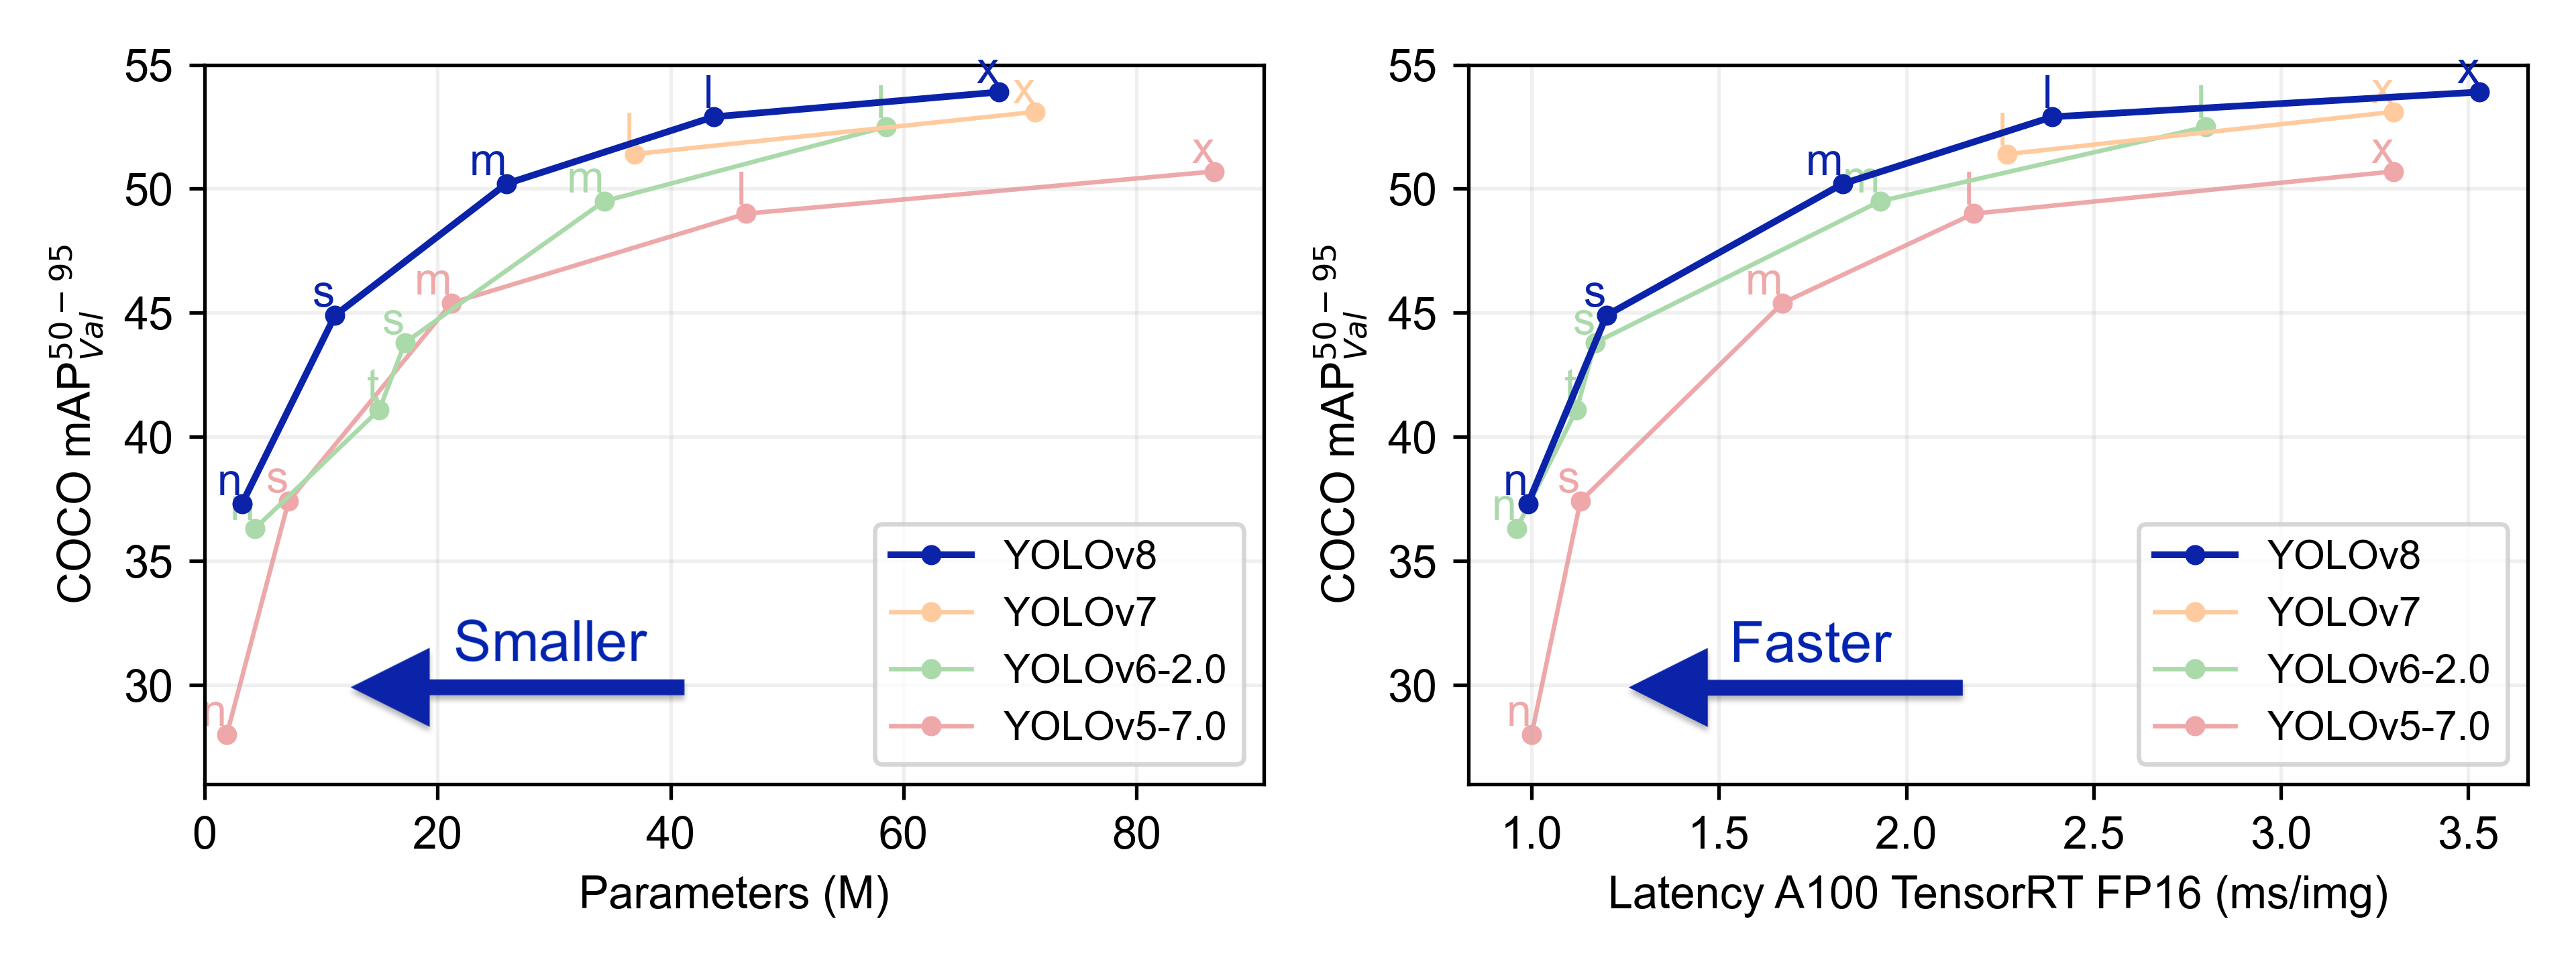
\includegraphics[width=120mm]{figures/yolo-comparison-plots.png}%

\begin{figure}[htb]%
	\centering%
	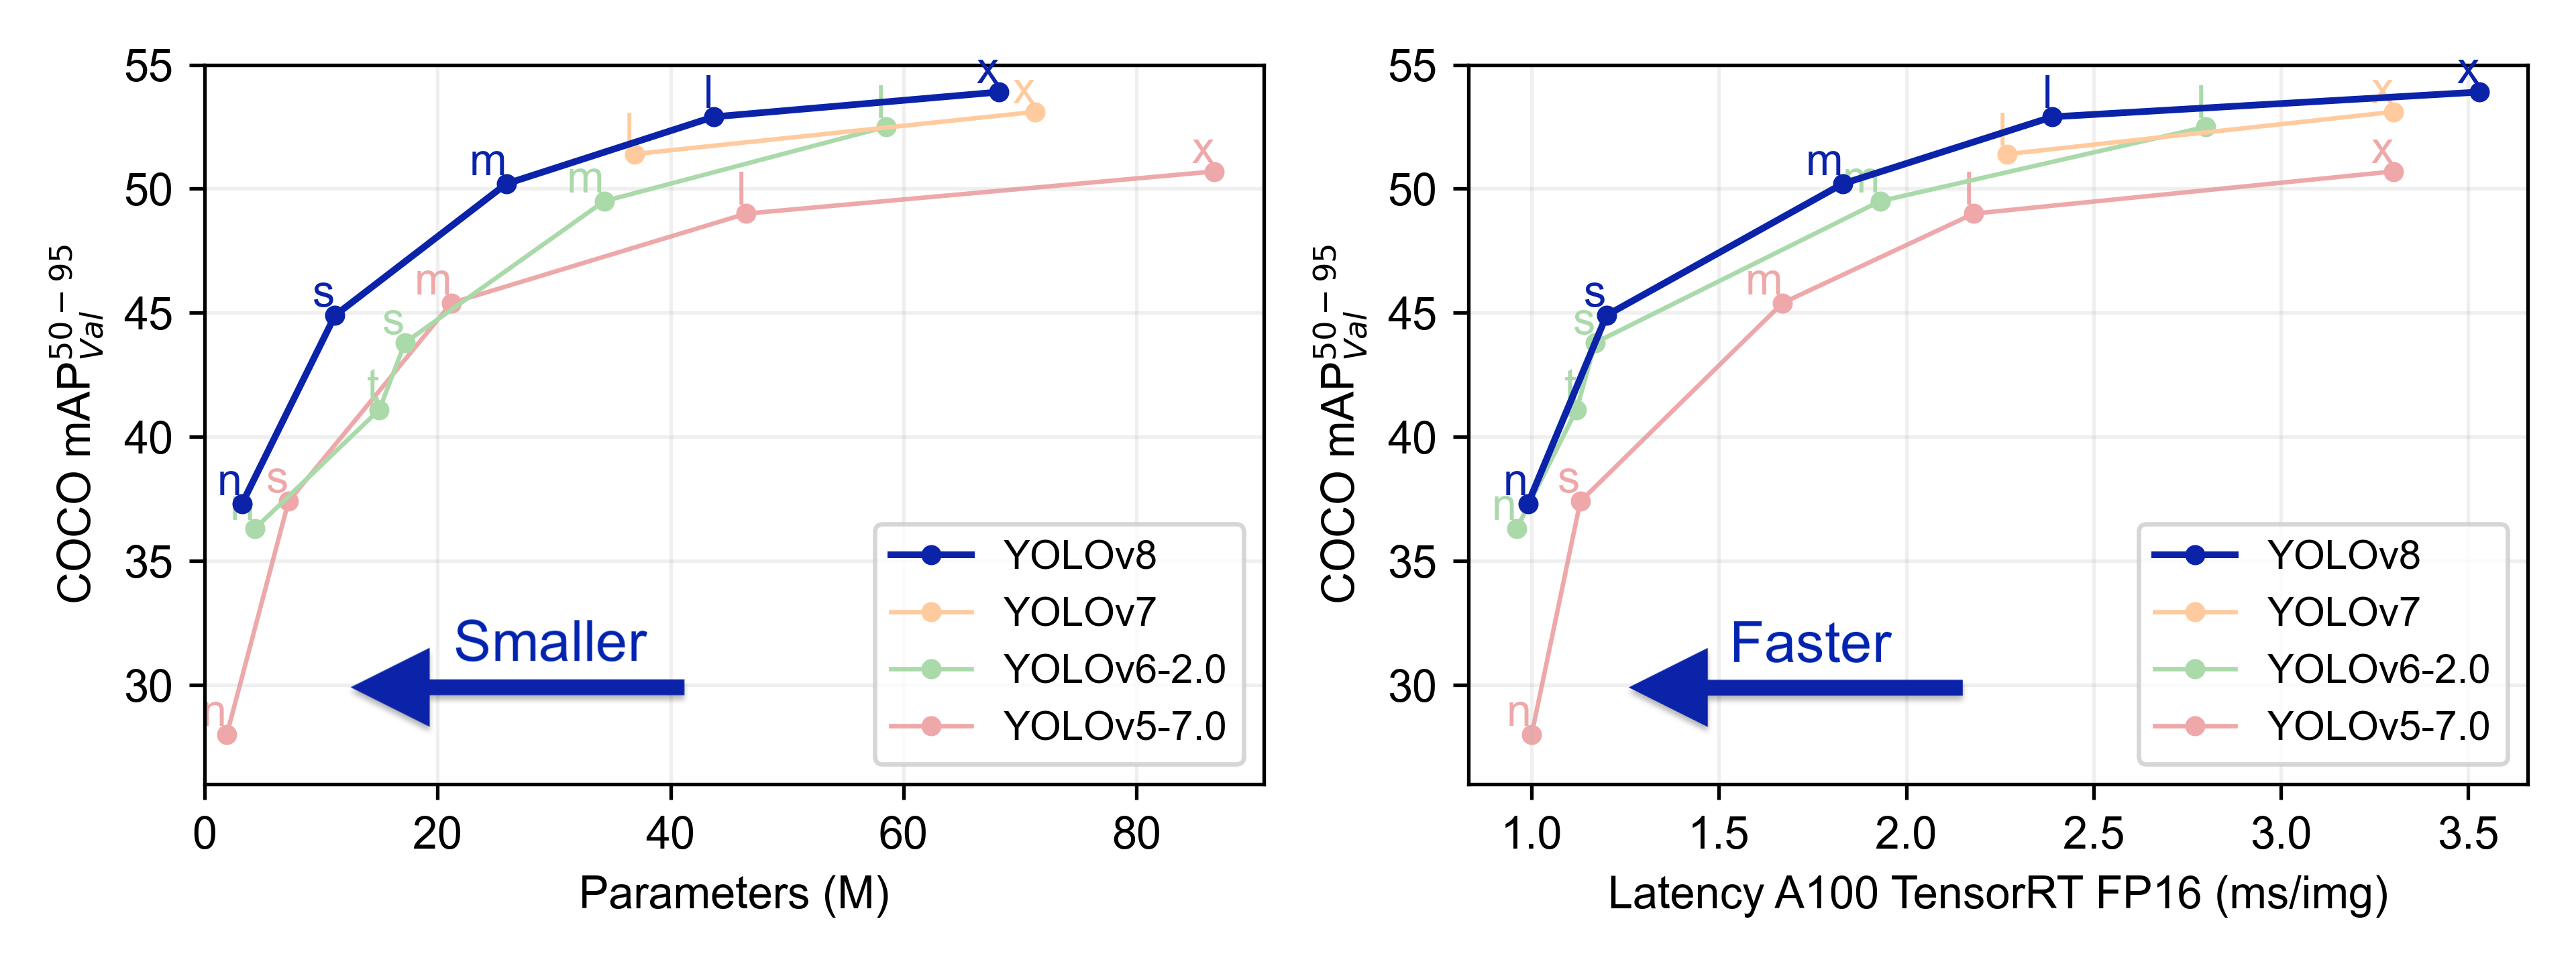
\includegraphics[width=150mm]{figures/yolo-comparison-plots.png}%
	\caption{YOLO parameters and latency comparison.}%
	\label{YOLO comparison}%
\end{figure}%

We choose the biggest model: YOLOv8x and additionally, we fine-tuned the models on our TUM Traffic dataset so that the model can detect all ten classes and improve the accuracy further. \hl{More on this in the dataset annotate and training section later.}

\subsection{TensorRT Optimization}

To preserve the real-time requirement of the Providentia system, we export the model to TensorRT to accelerate inference. NVIDIA’s TensorRT  \cite{vanholder2016efficient} is a high-performance deep-learning inference library designed to optimize and accelerate the inference of deep neural networks on NVIDIA GPUs. 

\section{C2F Seg}
\hl{TODO. Optional, if talk about C2F later}


\section{Annotation/Label Format}

- general description. Which formats will be presented. Which dataset use these formats? 
- we extended the TUMTraf dev-kit with label converters between these three format YOLO, COCO, OPENLabel. 

\subsection{OPENLabel Format}

The Association for Standardization of Automation and Measuring Systems (ASAM) with Deepen AI released the OpenLABEL  \cite{openlabel}, a standard designed to specify an annotation format flexible enough to support the development of automated driving features and to guarantee interoperability among different systems and providers. JSON schema is used to define the annotation structure of OpenLABEL and therefore annotation files are stored in .json format. 

TUMTraf dataset fully adopted this OPENLabel annotation format. \hl{Describe the TUMTraf annotation format with poly2d, bbox in with full and visible?}

\subsection{YOLO Format}

\subsection{COCO Format}
-  The annotations are stored using JSON.

\begin{mdframed}
	\textbf{COCO Annotation Format:}
	\begin{verbatim}
		{
			"annotation": {
				"id": int,
				"image_id": int,
				"category_id": int,
				"segmentation": RLE or [polygon],
				"area": float,
				"bbox": [x,y,width,height],
				"iscrowd": 0 or 1
			},
			"categories": [
			{
				"id": int,
				"name": str,
				"supercategory": str
			}
			]
		}
	\end{verbatim}
\end{mdframed}

%\begin{lstlisting}[caption={COCO Annotation Format}]
%	{
%		"annotation": {
%			"id": int,
%			"image_id": int,
%			"category_id": int,
%			"segmentation": RLE or [polygon],
%			"area": float,
%			"bbox": [x,y,width,height],
%			"iscrowd": 0 or 1
%		},
%		"categories": [
%		{
%			"id": int,
%			"name": str,
%			"supercategory": str
%		}
%		]
%	}
%\end{lstlisting}

\section{CVAT Labelling Tool}

To extend the TUMTraf Intersection Dataset with visible and full instance masks annotation, we use the open-source annotation tools CVAT (Computer Vision Annotation Tool) \cite{cvat} developed by Intel. 

Benefits: 
- CVAT allows users to annotate images with four types of shapes: boxes, polygons, polylines, and points. 
- CVAT supports multiple annotation formats including YOLO, MS COCO Object Detection, KITTI and many more. 
- CVAT supports automatic labeling by exploiting serverless deep learning model such as YOLO, RCNN, Face Detection, Segment Anything and many more. 

%
% !TeX spellcheck = en_US
\chapter{Implementation Details / Solution Approach}%

There are some big autonomous driving datasets with instance segmentation masks like NuScene, KITTI, Cityscape and COCO (sub-classes). Some of them were extended to amodal segmentation dataset (full mask) such as KINS dataset from KITTI and COCOA from COCO. The prior Providentia Mono3D system use YOLOv7 model pre-trained on COCO dataset. The new YOLOv8 model that is adapted in this work also have weights pre-trained on COCO. However, data in COCO has eighty classes, from which only six classes overlap with our TUM Traffic dataset. This possess some limitations. Firstly, occlusion with classes that are not considered in our dataset will cause big blobs in the detected mask.  \hl{add an example figure}. Secondly, the classes TRAILER, VAN and EMERGENCY \_VEHICLE are not in COCO and will either not be detected or detected with another classe label. To address these limitations, in this work, we propose training/ fine-tuning the 2d detector on our dataset. This will not only overcome the problem with unmatched classes but also lead to better detection as the model will learn to detect from our camera setting (angle, distance, etc.). 


\section{Visible and full instance segmentation annotation for TUMTraf dataset}

TUMTraf dataset has 2D keypoints and 3D bounding box labels but no segmentation masks, so we can not directly use the dataset to train instance segmentation models. In this work, we extended the TUM Traffic Intersection dataset with visible and full instance mask labels. The OpenLABEL annotation schema for TUMTraf dataset is extended like the following: \hl{show the extended masks and visible boxes}. The additionaly \code{poly2d} contains the full and visible masks. The masks are stored as lists of 2D coordinate of the polygon contours. The \code{bbox} is extended with a full bounding box. 

And how did we set the value for the instance masks? We use YOLO pre-trained on COCO to automatically detect the objects visible masks. The detections were then loaded into Computer Vision Annotation Tool (CVAT), where the visible masks will be manually refined and extended to full masks. We have tried our best to accurately annotate the full mask by searching for the objects occludded part in another frame where it is visible. This manually annotation process was only done for each tenth frames (10\% of the dataset), the remaining frames in the middle were annotated automatically with a simple 2D detection interpolation pipeline. This works and is meaningful because, as described earlier in section 3.2, the TUMTraf Intersection dataset contains four scenes (videos), so interpolation makes scene and works.   

The frames are first sorted in ascending chronological order, then for each pair of consecutive labeled frames, the objects annotations are interpolated from the first frame to the second frame. The steps can be summarized as follow: 
\begin{enumerate}
	\item A 2D distance matrix $D$ of shape $N \times M$  is created, with $N$ and $M$  are the amount of object's annotation of first frame and second frame respectively. Each cell $D[i,j]$ is the straight-line distance (aka. Euclidean distance) of the center of the i-th object from first frame to the center of the j-th object from second frame. In case the categories of the two objects are not identical, the distance is set to infinity. 
	
	\[ D(i,j) = \begin{cases} 
		\sqrt{{(x_{\text{{center}}_i} - x_{\text{{center}}_j})^2 + (y_{\text{{center}}_i} - y_{\text{{center}}_j})^2}} & \text{if } \text{{category}}_i = \text{{category}}_j \\
		\infty & \text{otherwise}
	\end{cases} \]
	
	This matrix is then given to \code{scipy.optimize.linear\_sum\_assignment()}to match each object annotation of the first frame to one object annotation of the second frame. The \code{scipy.optimize.linear\_sum\_assignment()} function exploits the Jonker-Volgenant algorithm to match objects with minimal distance. %\cite{scipyLSA} 
	
	\item For each pair of matched object annotations, the visible and full masks are interpolated. We again match each polygon point of the first object mask with one polygon point of the second object mask. Then linear interpolation is used to interpolate each single polygon point. 
	
	\[
	x_k = x_0 + \frac{{x_1 - x_0}}{{n + 1}} \cdot k
	\]
	\[
	y_k = y_0 + \frac{{y_1 - y_0}}{{n + 1}} \cdot k
	\]
	
	With \(n\) being the number of un-annotated frames in the middle, \(k \in [1, n]\), and \((x_0, y_0)\) and \((x_1, y_1)\) being the matched polygon point from the first frame and the second frame, respectively.
	
	\item Bounding boxes are then calculated from the masks, object category and other attributes are copied over.  
\end{enumerate}

This 2D detection interpolation pipeline is not just copying and pasting the bounding boxes and masks and interpolate the position. Each point of the polygon contour of the mask is interpolated individually. Thereby, not only the position, but also the shape and rotation of the object are interpolated and provide much more accurate labels that do not require too much refinement later \hl{add an example figure}. 

One limitation/ challenge that can still be improved is the matching of objects from the first frame to objects from the last frames. The current used linear sum assignment problem approach fails when not all objects in the first frame are still exit in the last fram and vice versa \hl{add an example figure}. Besides, one false matching can lead to a chain of errors since each object can only be matched to one other object \hl{add an example figure}. One possible solution/ future work would be to exploit tracking algorithm to better match/track objects between frames. 


\section{Fine tune YOLOv8x-seg on TUMTraf dataset}
- train using a batch size of ... on ... 
- The total number of iterations is set to ...
- following the standard ...

\section{Export YOLO models to TensorRT and integrate into the toolchain}

\section{Fine tune C2F\_seg on TUMTraf dataset}



%
% !TeX spellcheck = en_US
\chapter{Evaluation / Experimentsk}%
- In order to evaluate the performance 
- we conduct experiments on 
- All experiments are conducted on a single 2080Ti GPU card
- For 512×512 images, E2EC achieved a 36 fps inference speed on an NVIDIA A6000 GPU

\section{Evaluation Metrics}

- 2D object detection / segmentation:  Average Precision (AP) 
- 3D object detection (Providentia Mono3D): also  Average Precision (AP) 



- We choose the mean Intersection over Union (mIoU) and mean Average Precision (mAP) as metrics for performance evaluation
- For evaluation, we adopt standard metrics as in most amodal segmentation literature , namely mean average precision (AP). Furthermore, We use mean-IoU to measure the quality of predicted masks.
- In this paper, the mask quality is evaluated in terms of the standard AP metric.

\section{Quantitative results}


\section{Qualitative results}

\section{Inference Speed}

- 1-2 sentences: what is TensorRT
- Pytorch model → tensorRT

- Model performance on RTX-3090 GPU
- Yolov7-640 models achieve frame-rates between 55 and 60 FPS on the RTX-3090 GPU
- Yolov7-1280 achieves 22 FPS, and Yolov7-1920 reaches only 12 FPS
- how many \% speed up? TensorRT vs. .pt


- problems with detecting the instance masks of large objects near the camera.%
% !TeX spellcheck = en_US
\chapter{Experiments}  \label{chap:six}%%

\section{Performance on Night sequence} \label{sec:night_sequence}

\begin{table}[htb]%
	\begin{subfigure}{\textwidth}
		\centering
		\begin{subfigure}{0.245\textwidth}
			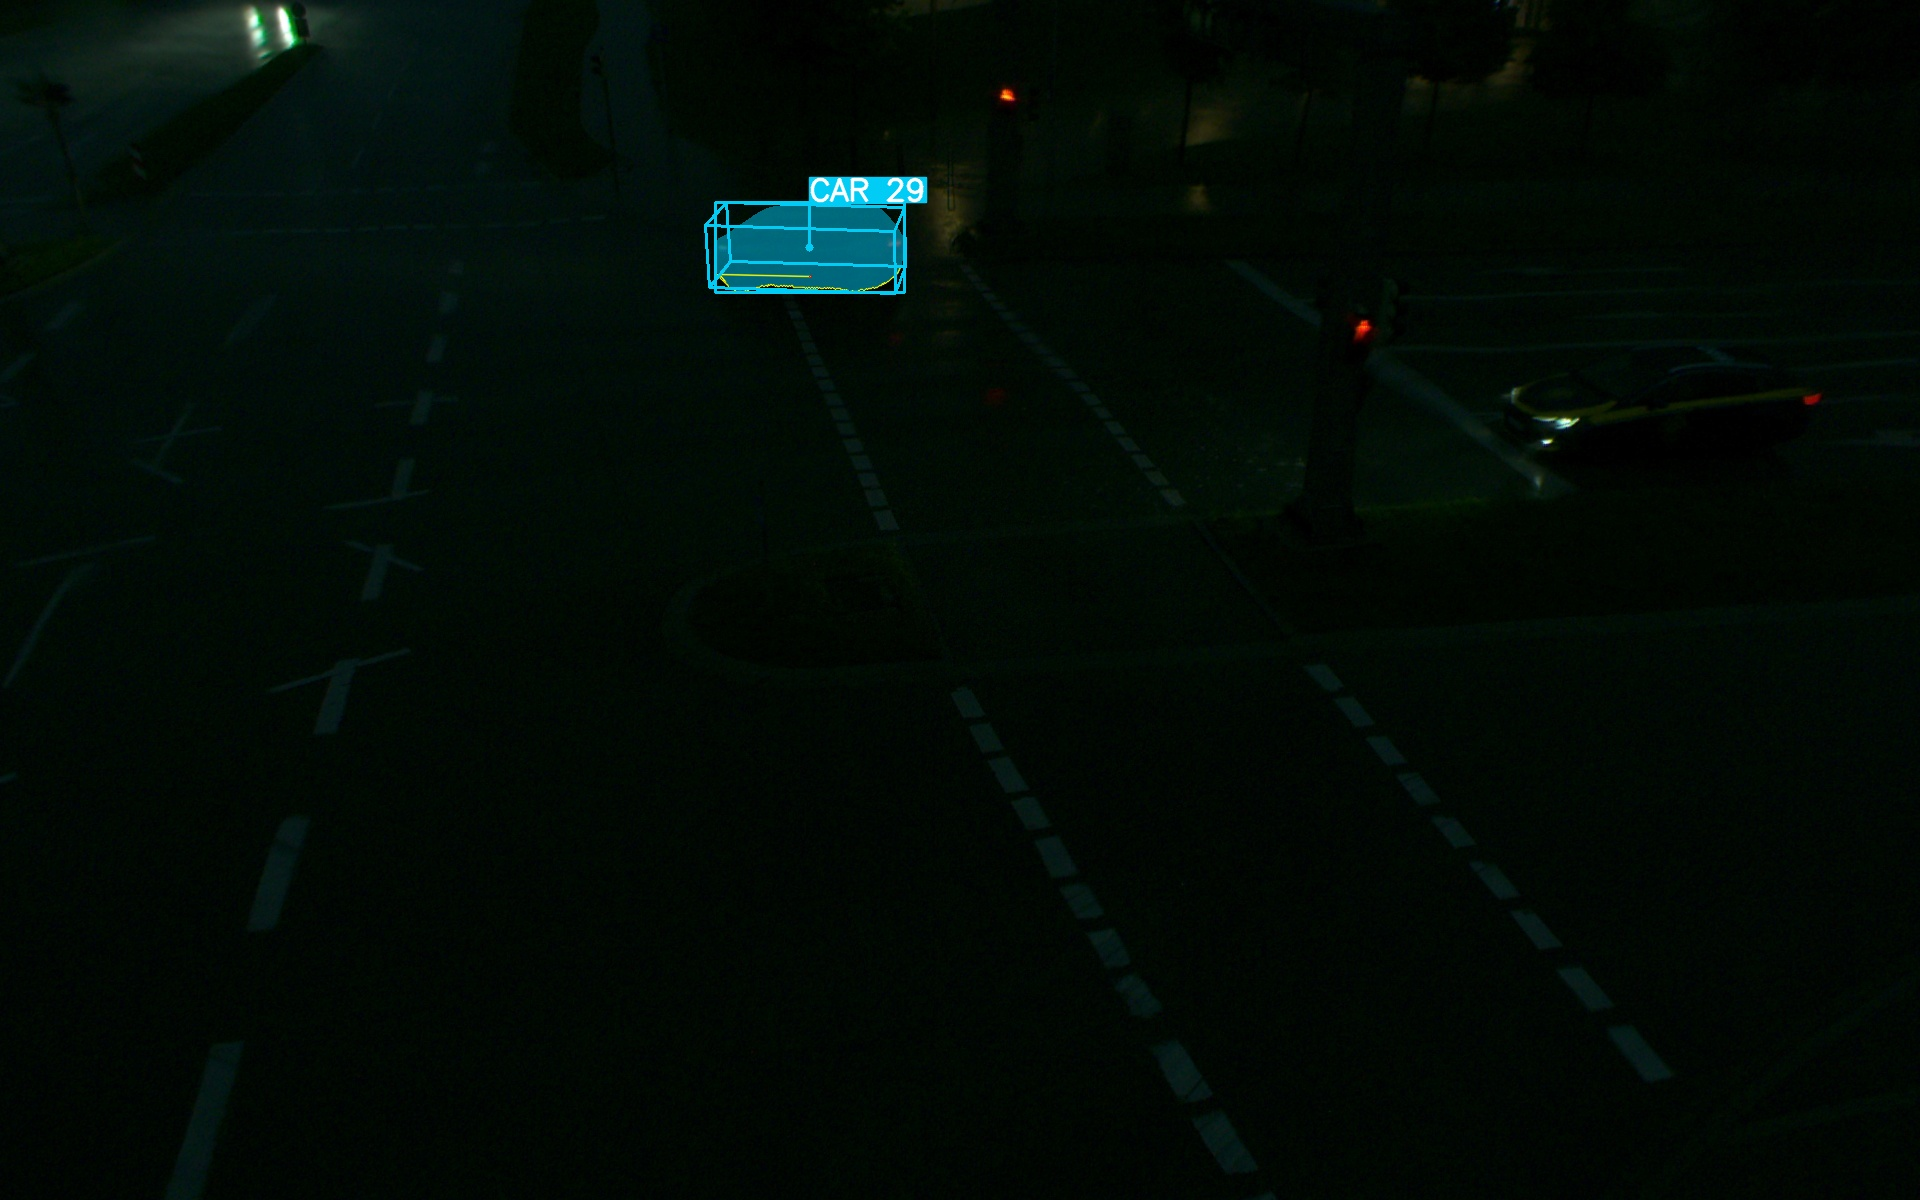
\includegraphics[width=\linewidth]{night_stable1_yolov7.jpg}
		\end{subfigure}\hfill
		\begin{subfigure}{0.245\textwidth}
			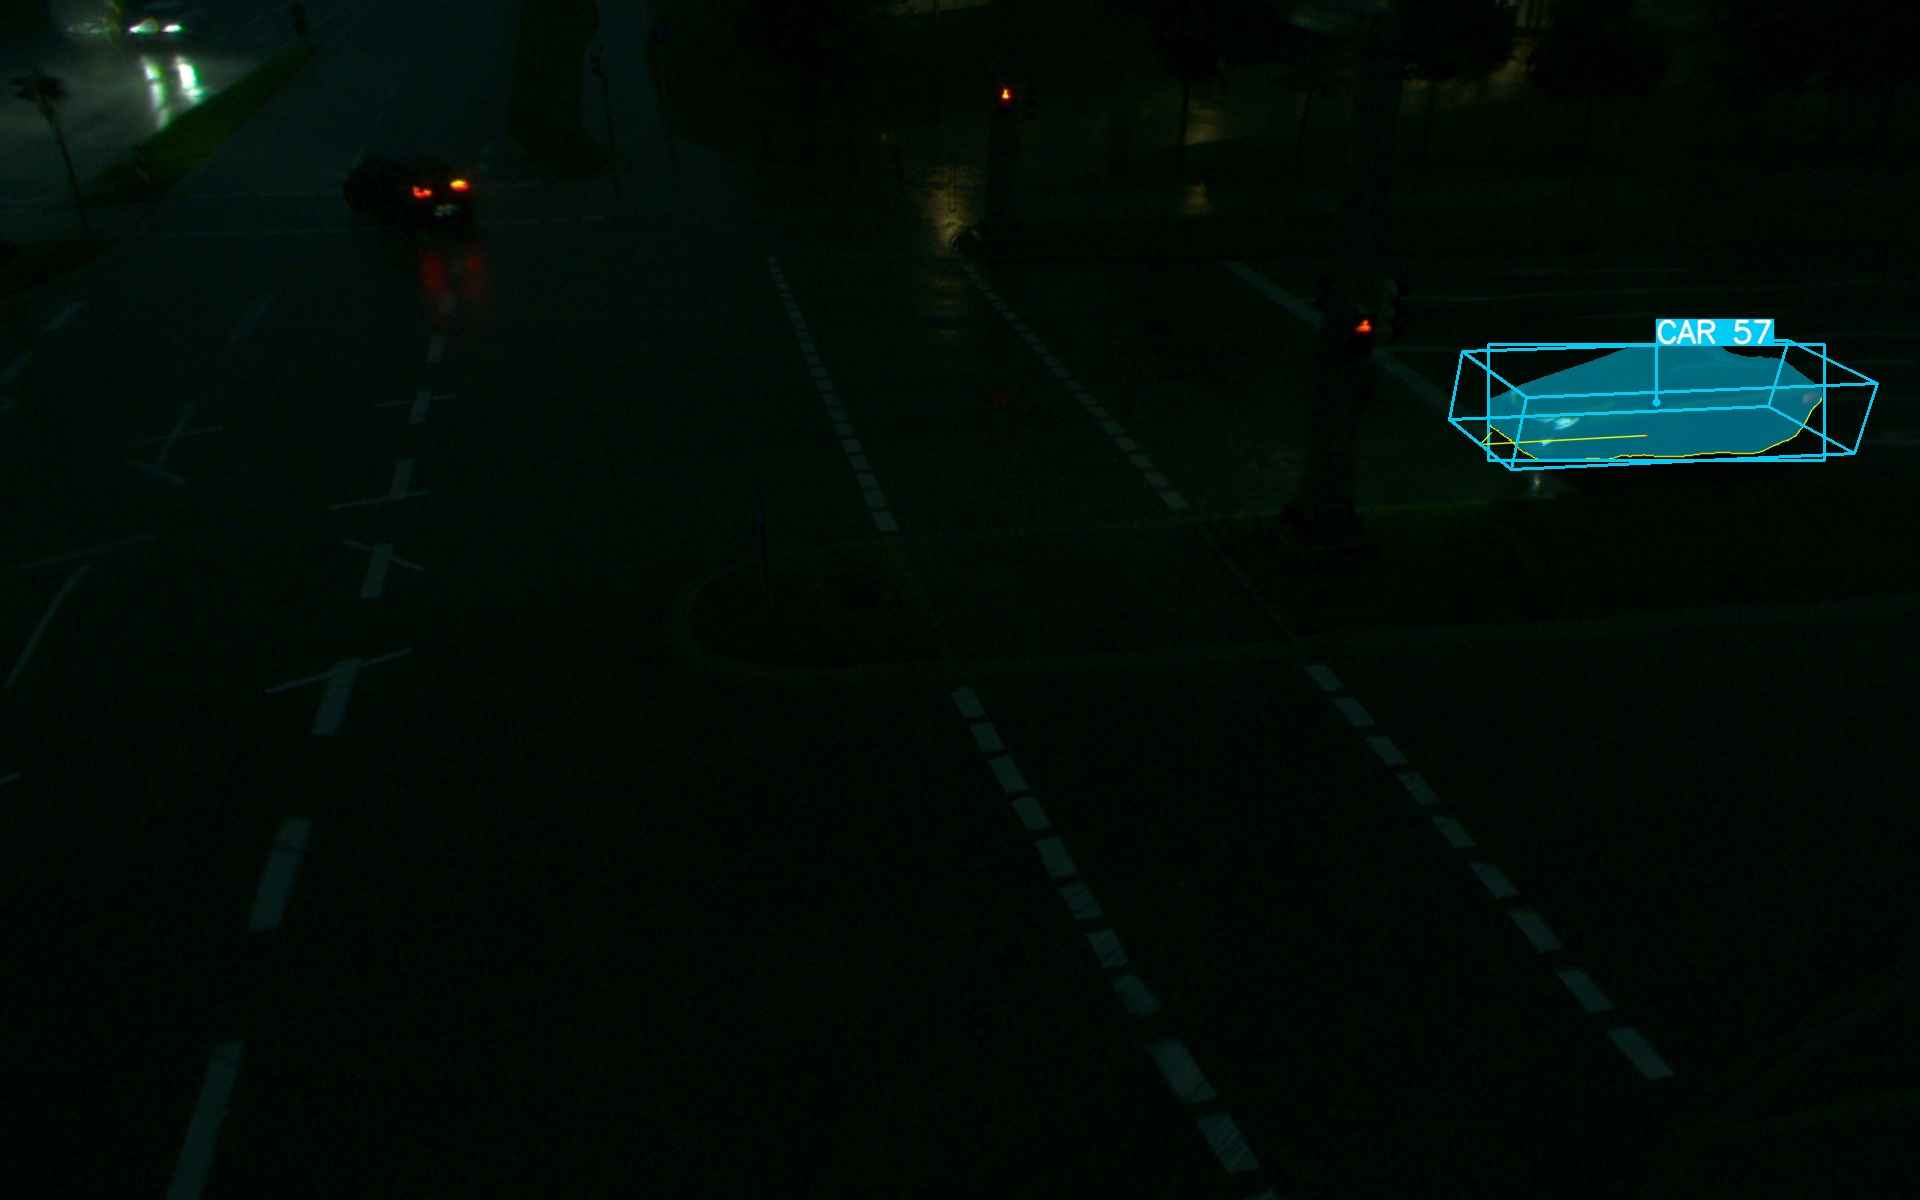
\includegraphics[width=\linewidth]{night_stable2_yolov7.jpg}
		\end{subfigure}\hfill
		\begin{subfigure}{0.245\textwidth}
			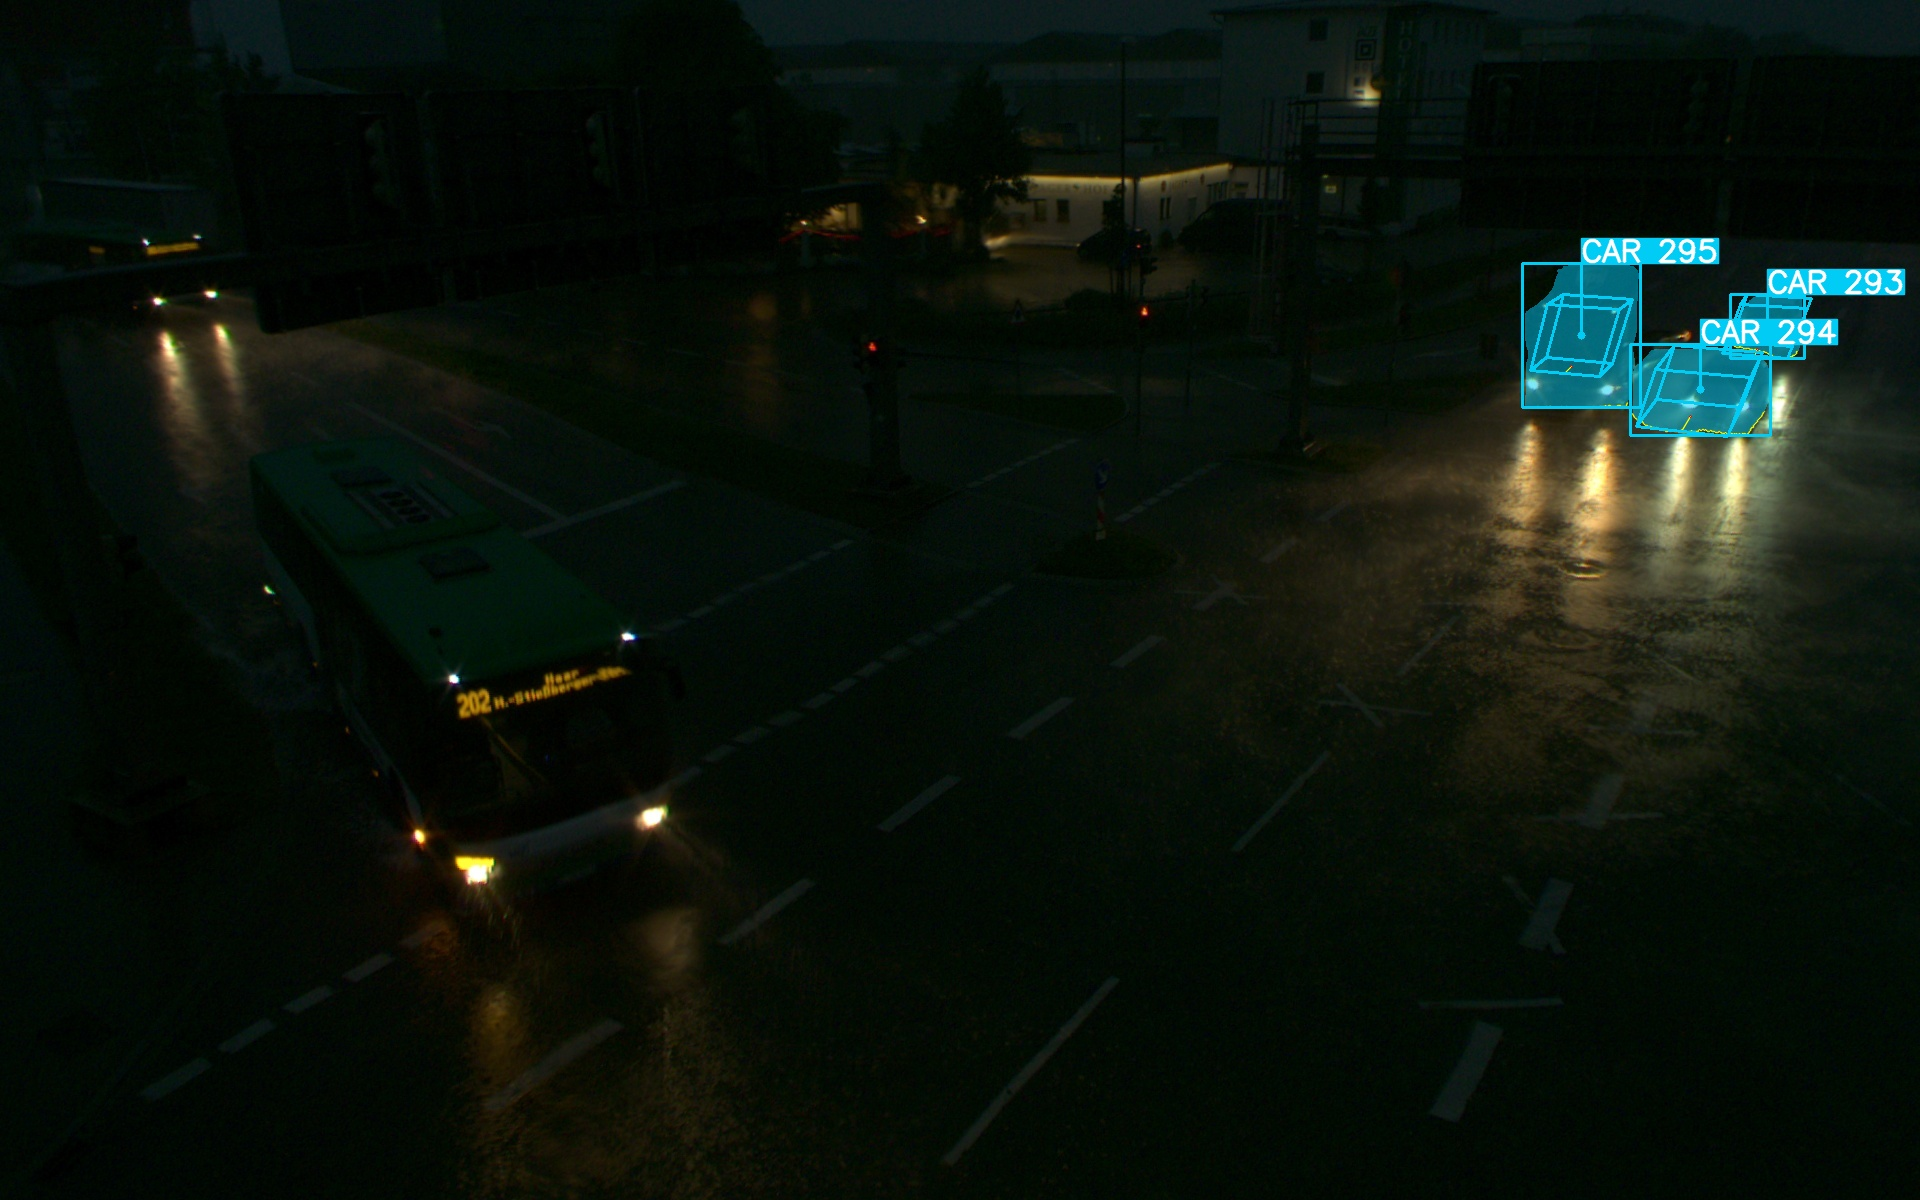
\includegraphics[width=\linewidth]{night_bus_yolov7.jpg}
		\end{subfigure}\hfill
		\begin{subfigure}{0.245\textwidth}
			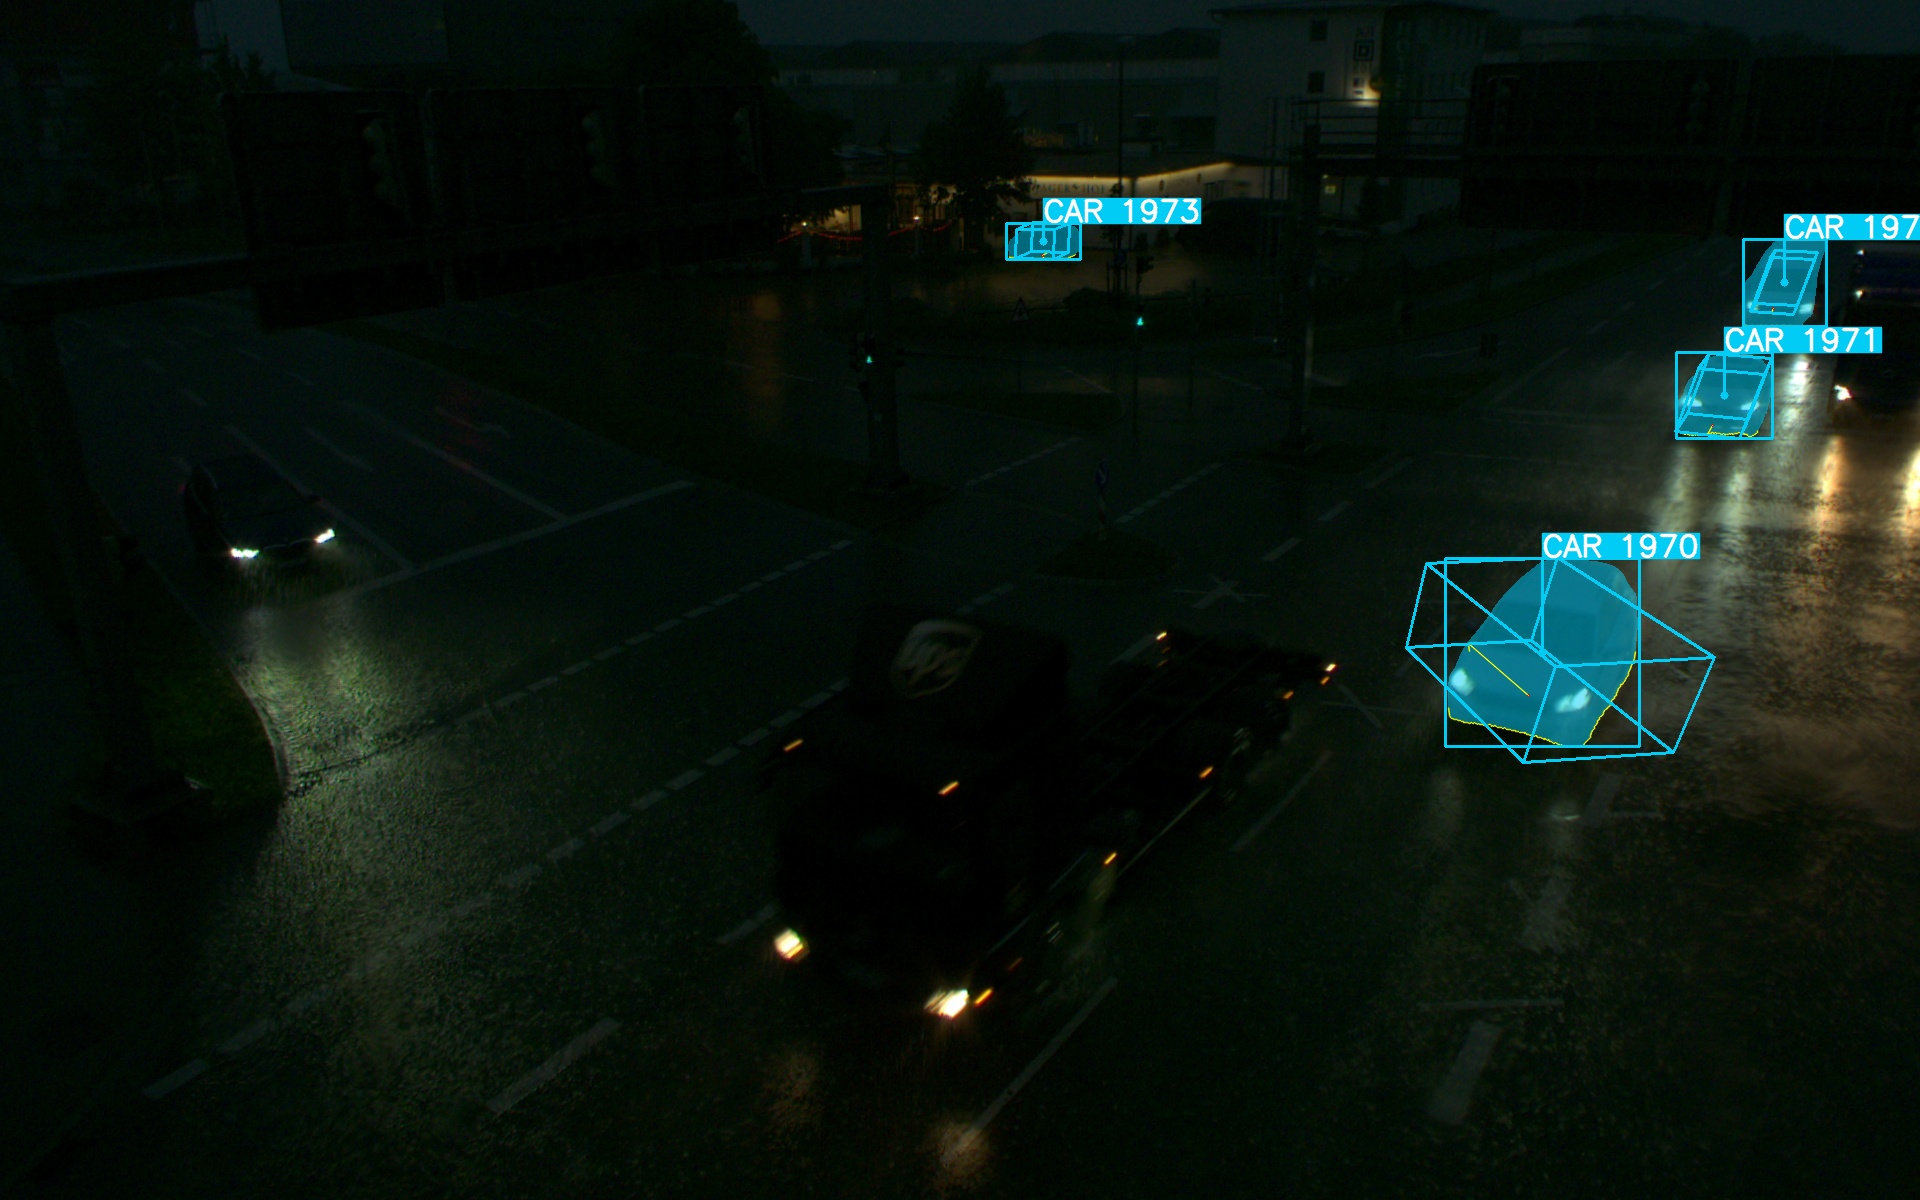
\includegraphics[width=\linewidth]{night_yolov7.jpg}
		\end{subfigure}
		%\caption{\small $YOLOv7\_coco$}
	\end{subfigure}
	
	\begin{subfigure}{\textwidth}
		\centering
		\begin{subfigure}{0.245\textwidth}
			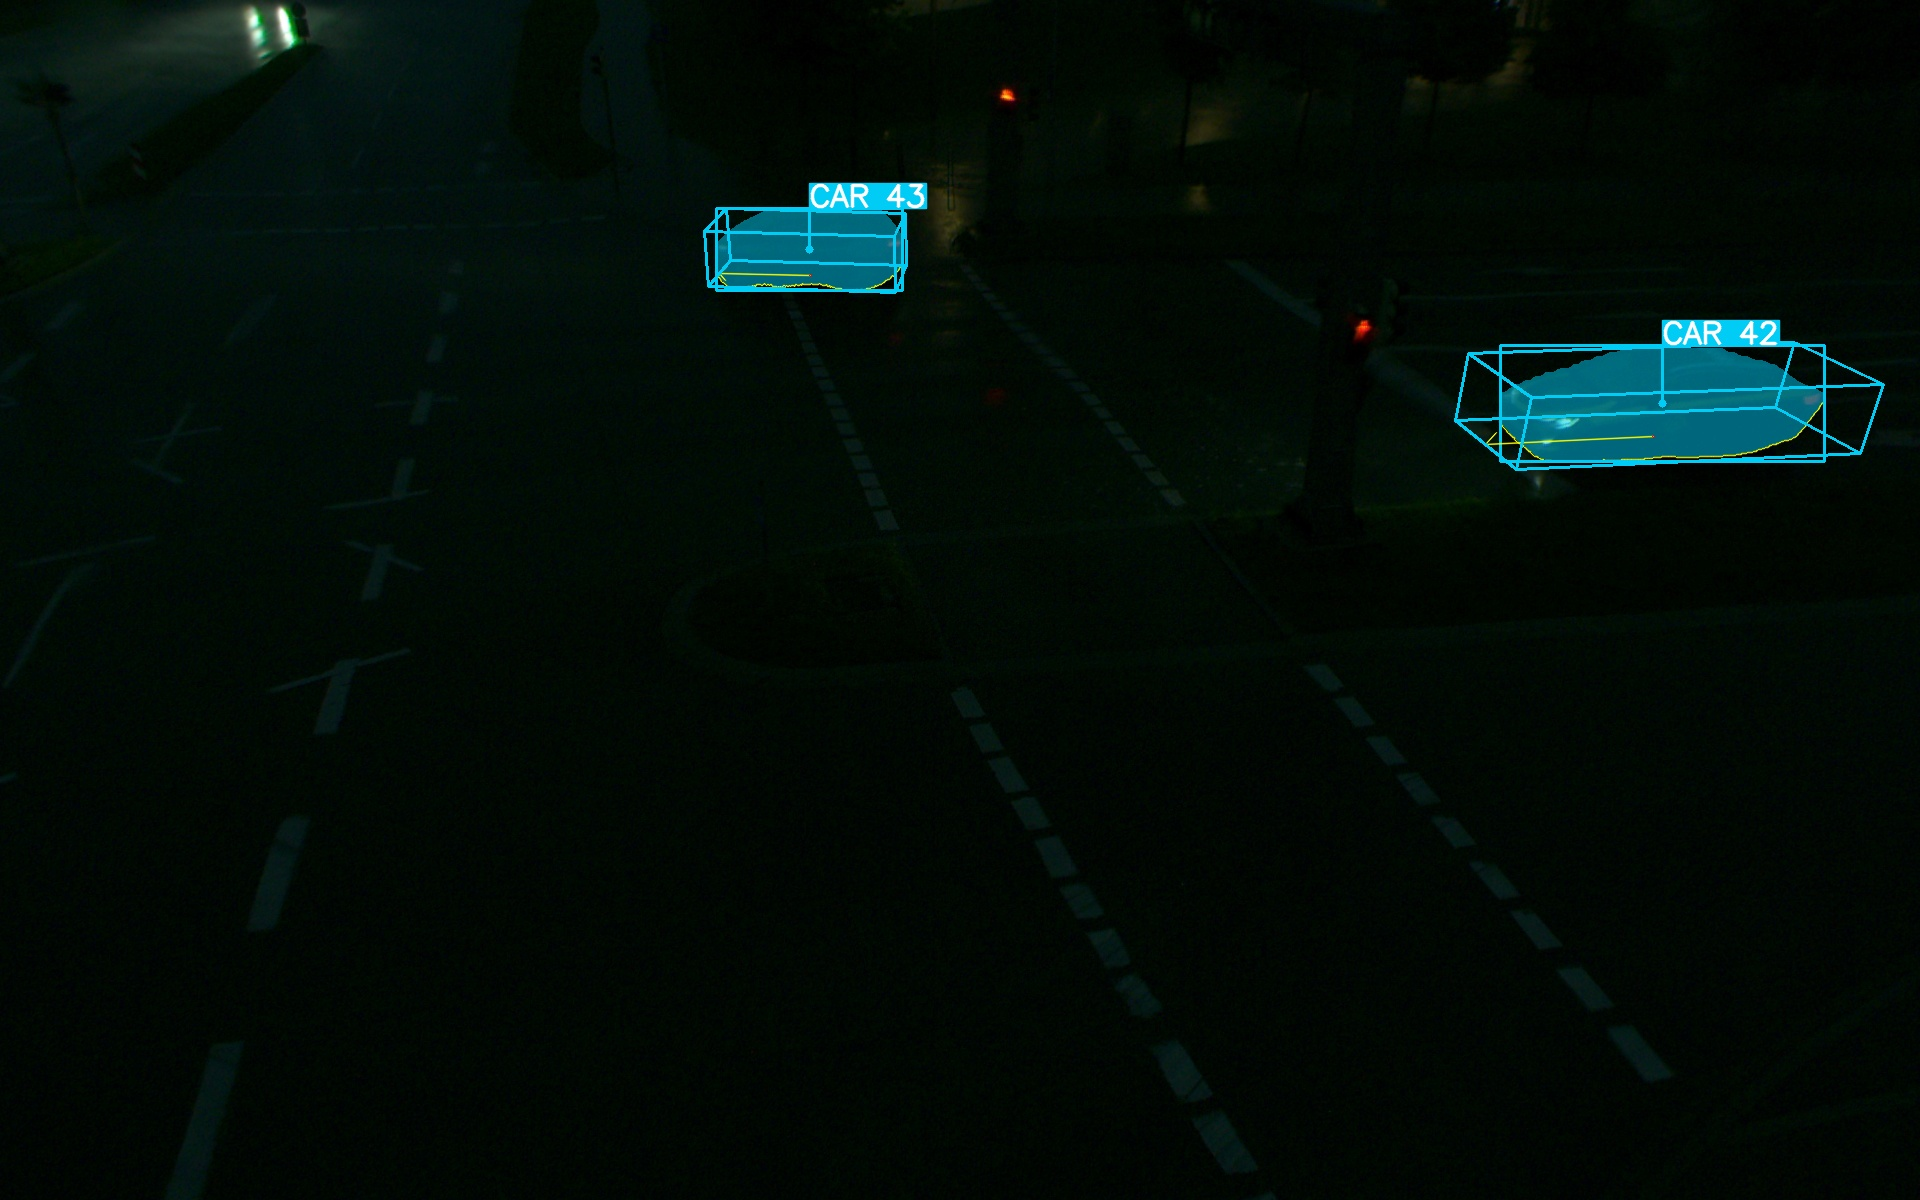
\includegraphics[width=\linewidth]{night_stable1_yolov8_scratch.jpg}
		\end{subfigure}\hfill
		\begin{subfigure}{0.245\textwidth}
			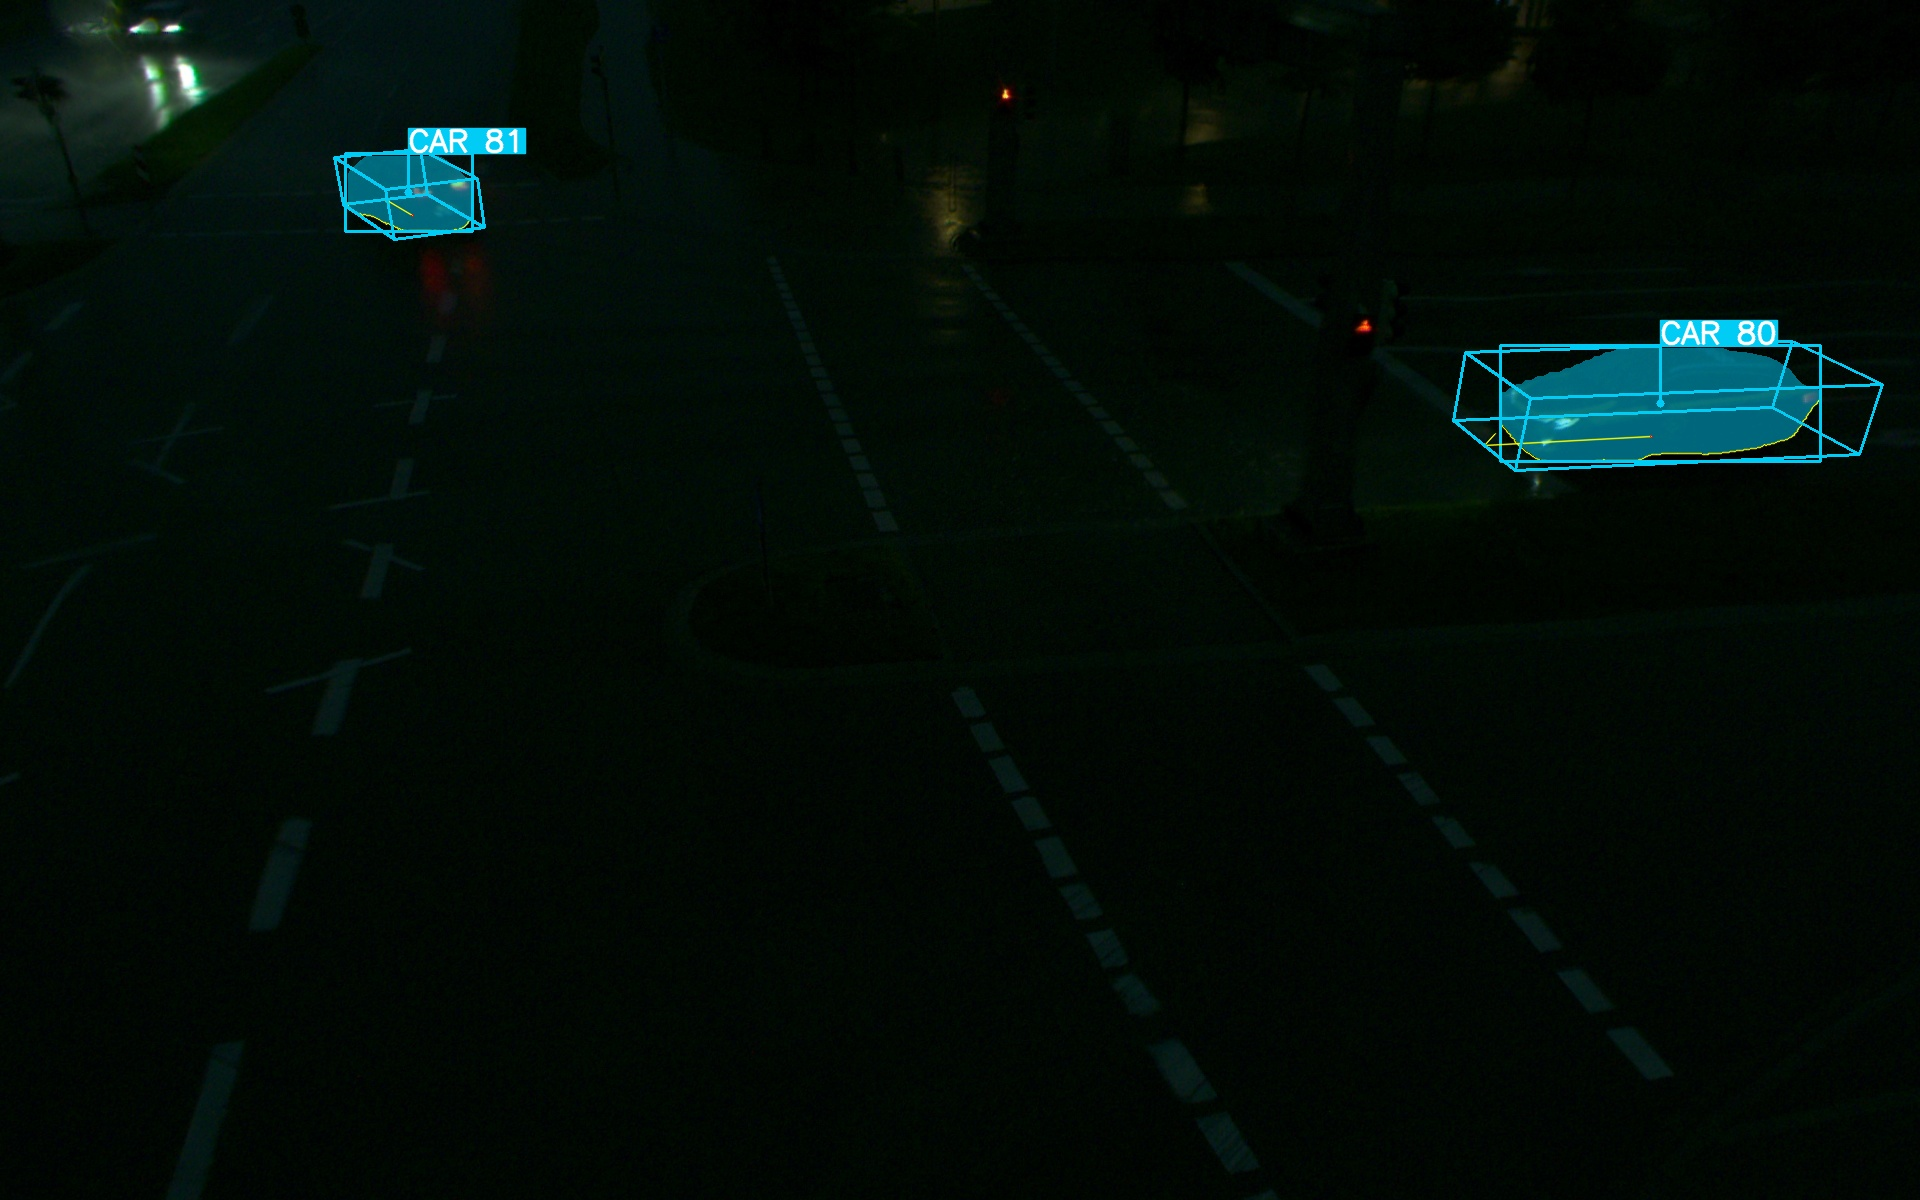
\includegraphics[width=\linewidth]{night_stable2_yolov8_scratch.jpg}
		\end{subfigure}\hfill
		\begin{subfigure}{0.245\textwidth}
			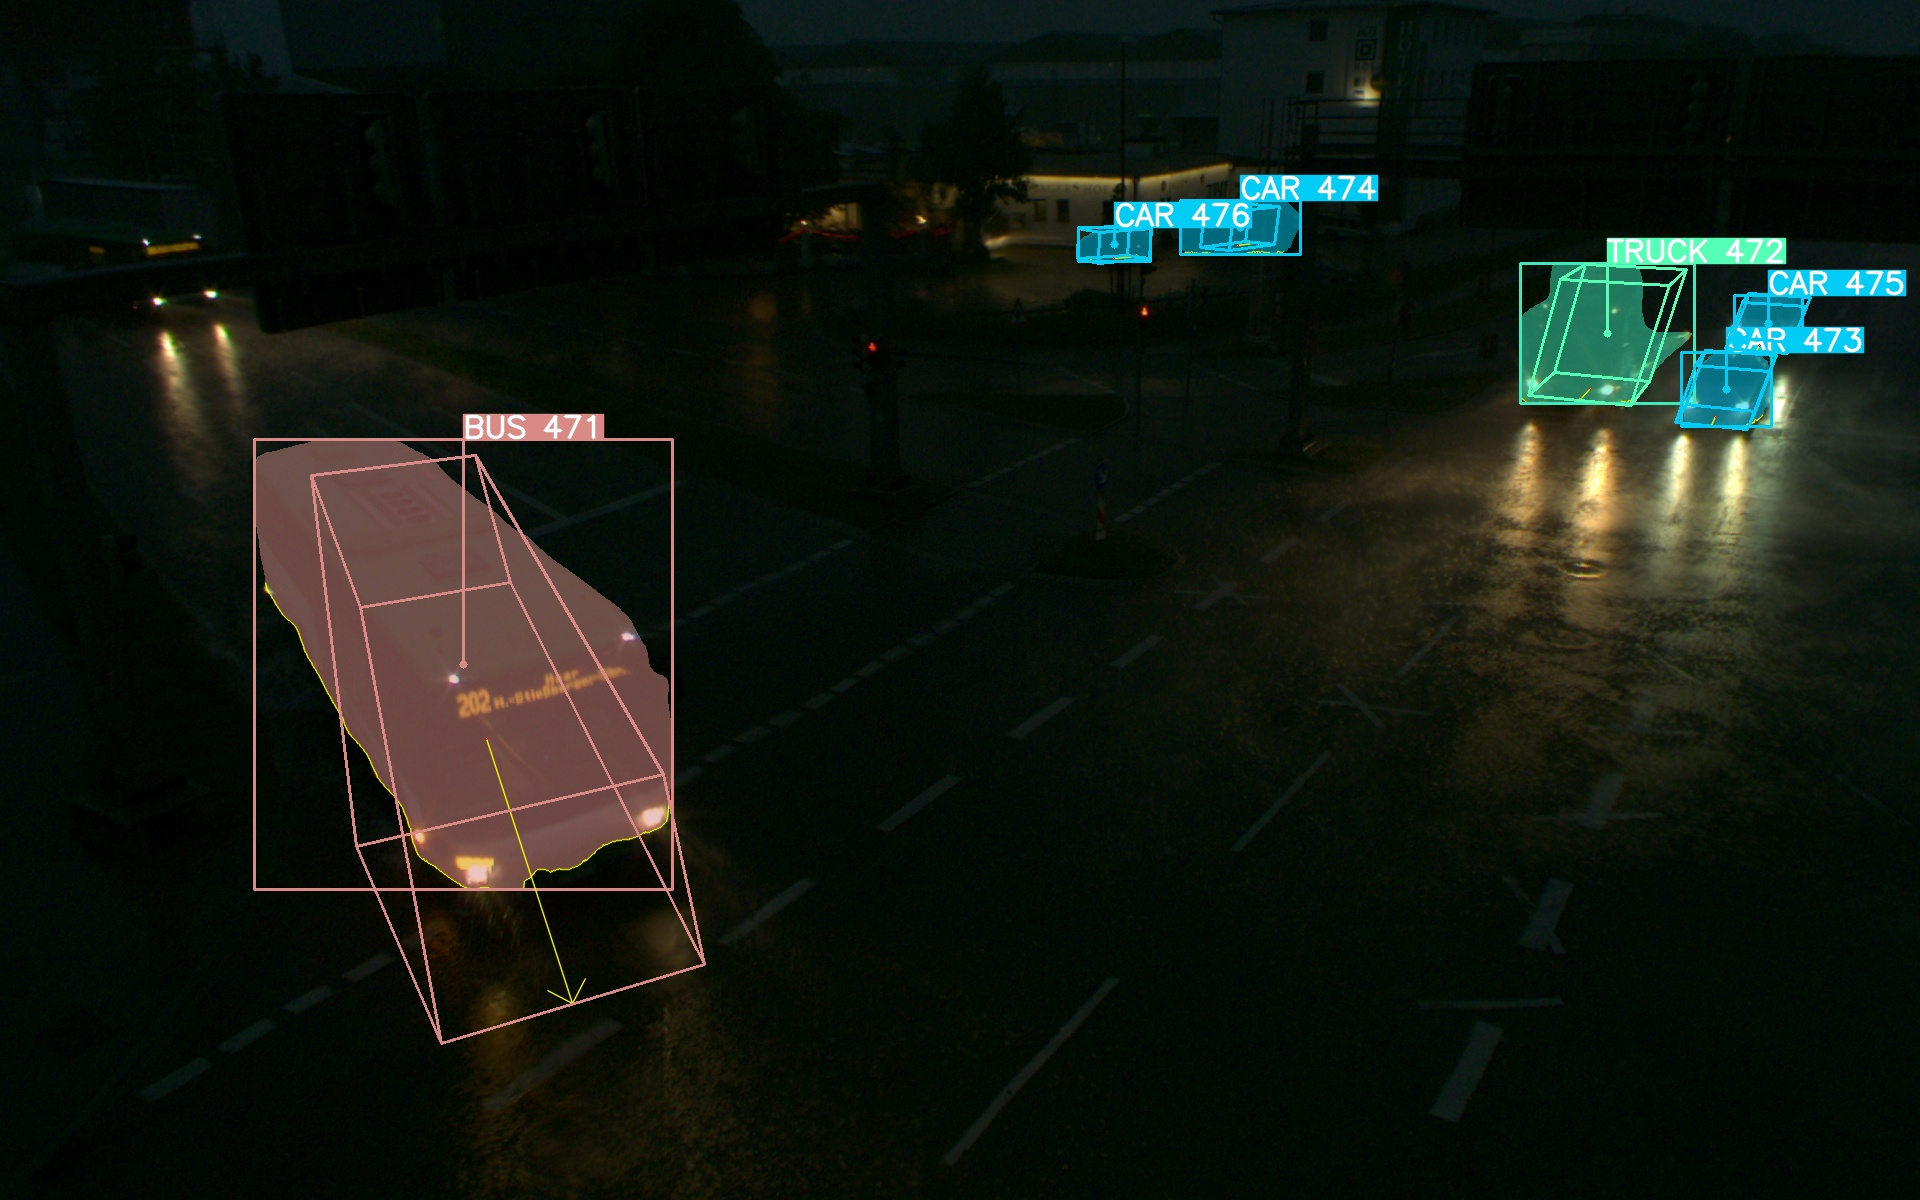
\includegraphics[width=\linewidth]{night_bus_yolov8_scratch.jpg}
		\end{subfigure}\hfill
		\begin{subfigure}{0.245\textwidth}
			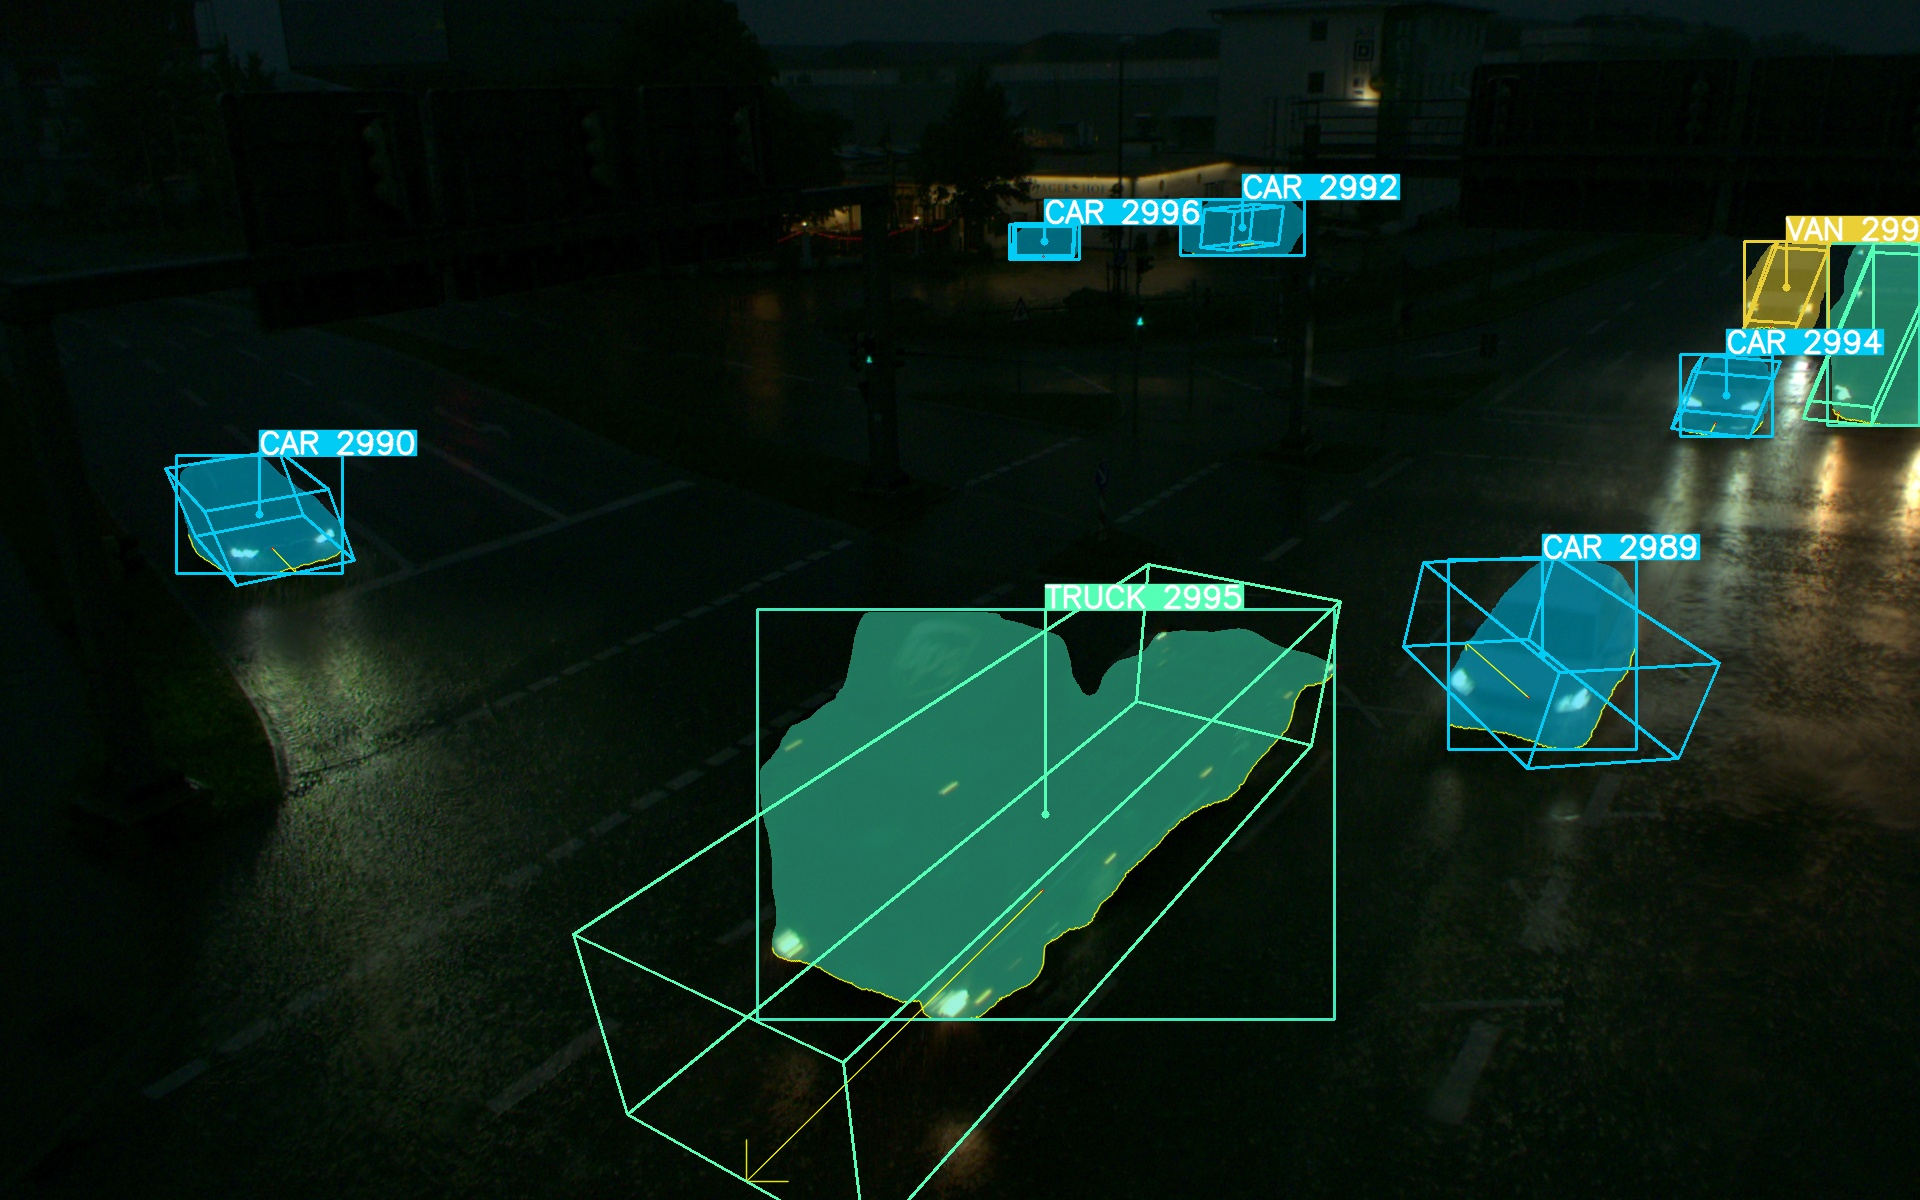
\includegraphics[width=\linewidth]{night_yolov8_scratch.jpg}
		\end{subfigure}
		%\caption{\small $YOLOv8x\_tumtraf$}
	\end{subfigure}
	
	\begin{subfigure}{\textwidth}
		\centering
		\begin{subfigure}{0.245\textwidth}
			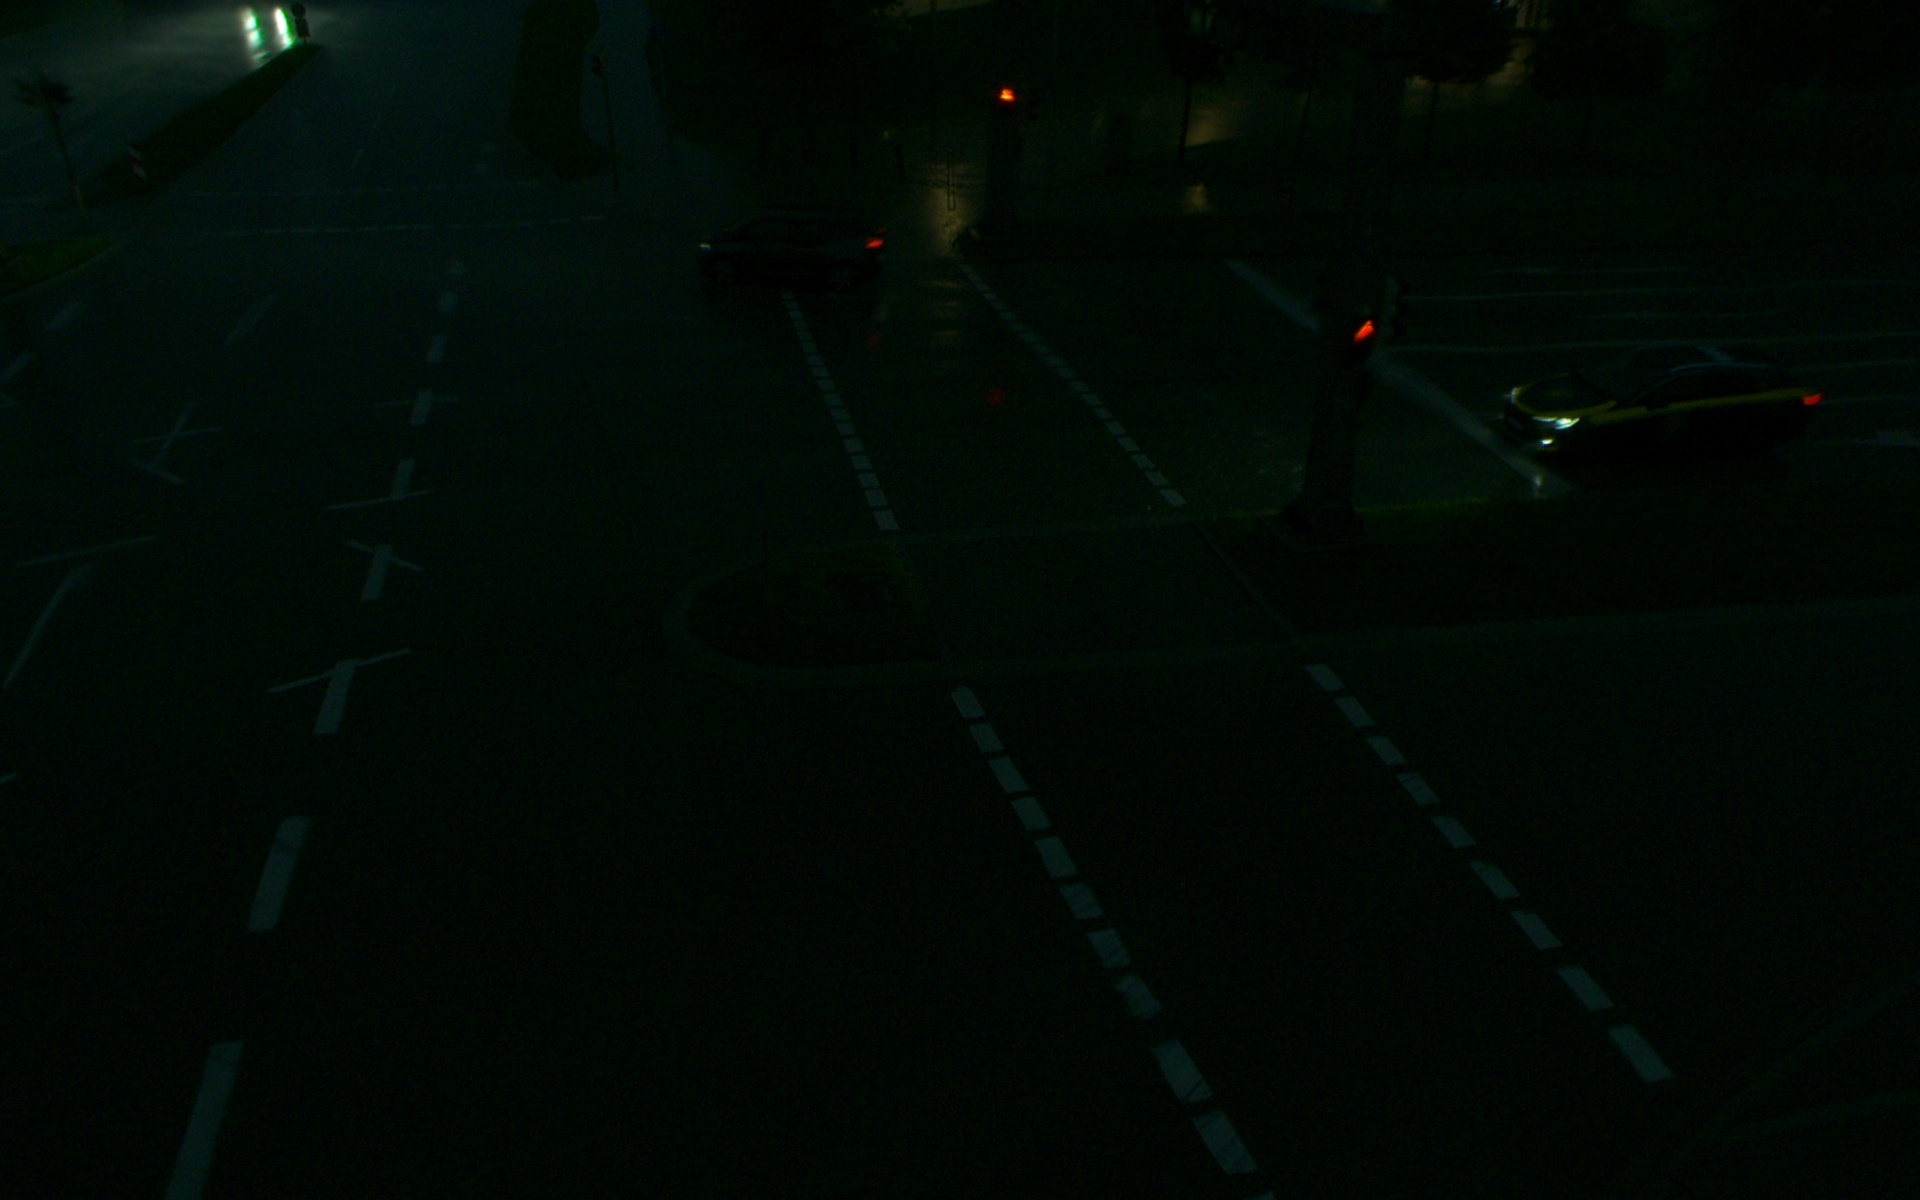
\includegraphics[width=\linewidth]{night_stable1_yolov8_finetuned.jpg}
		\end{subfigure}\hfill
		\begin{subfigure}{0.245\textwidth}
			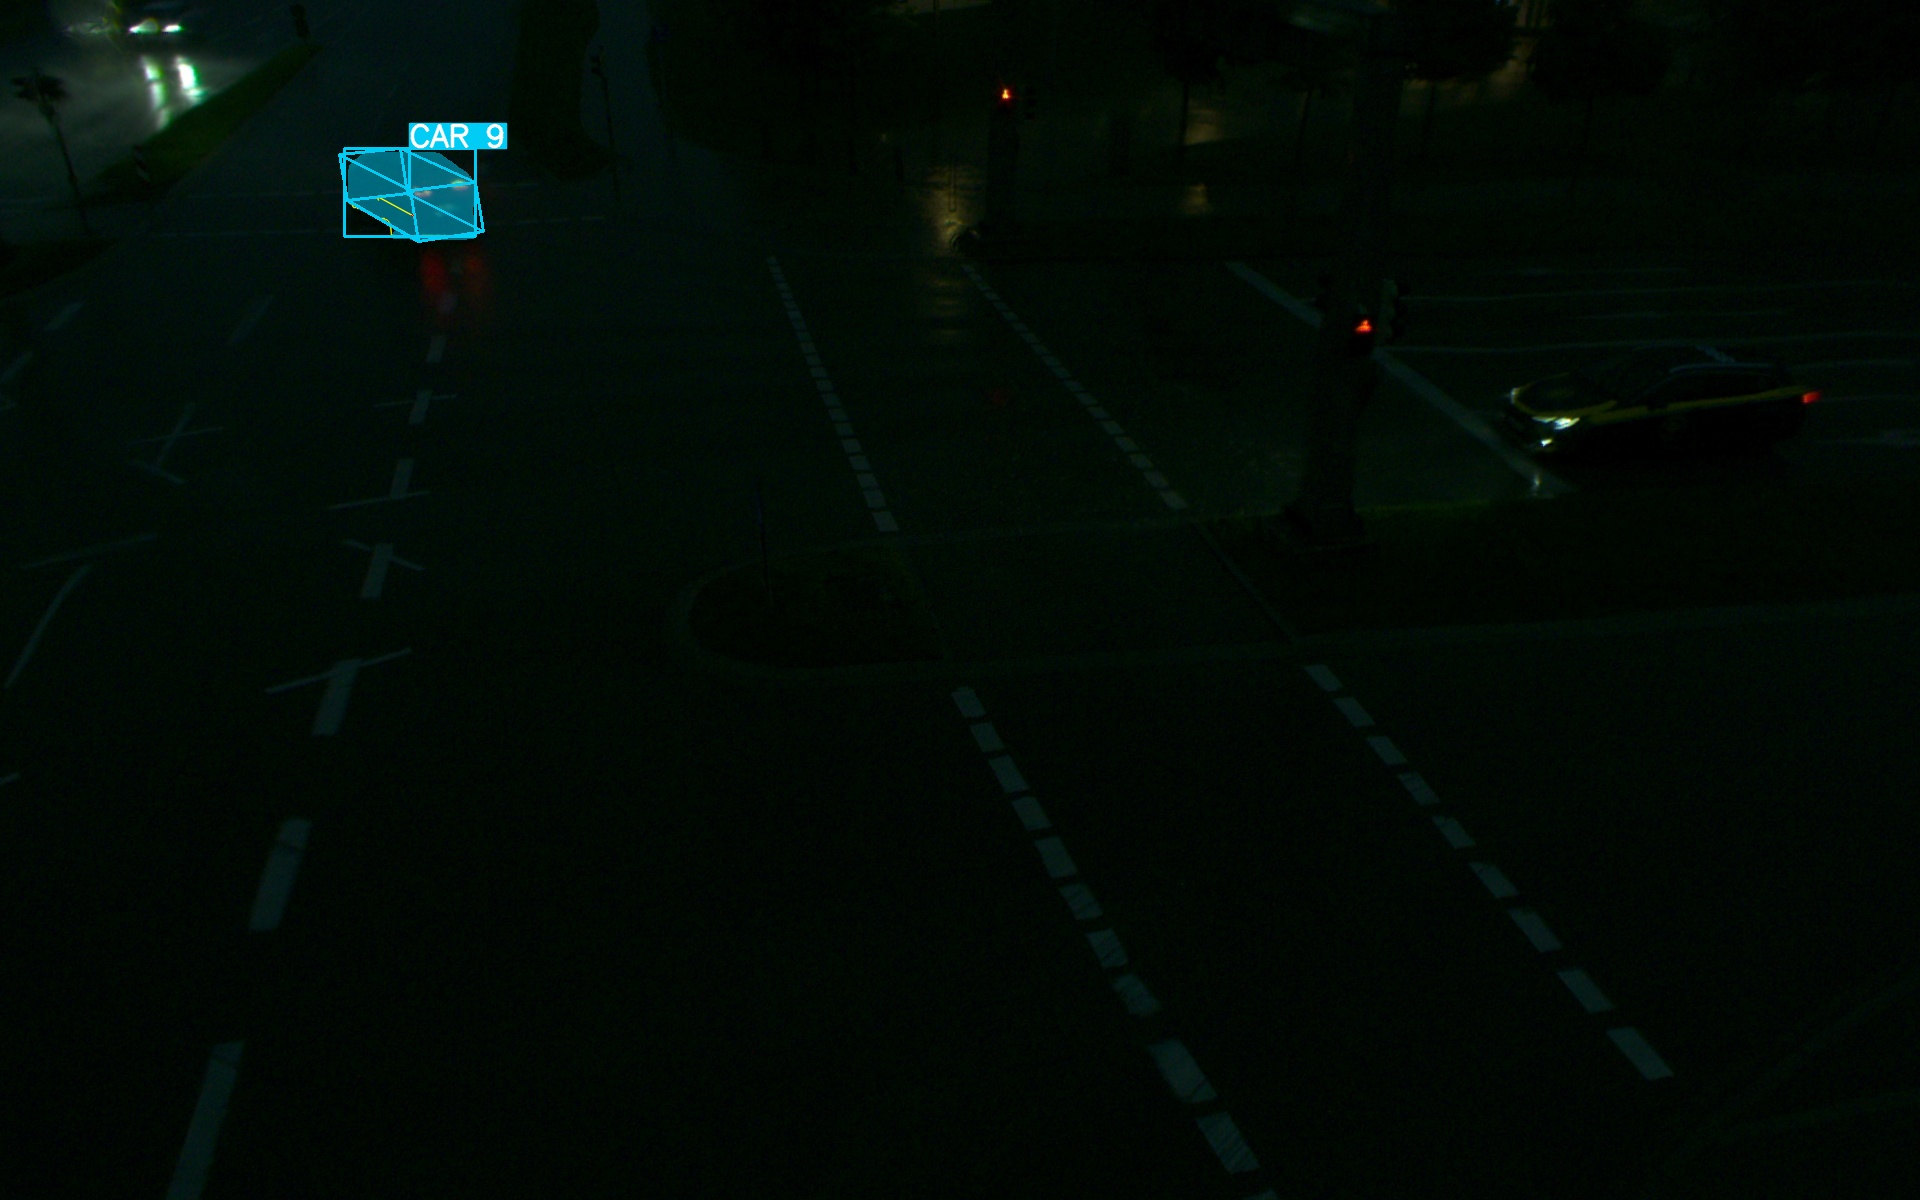
\includegraphics[width=\linewidth]{night_stable2_yolov8_finetuned.jpg}
		\end{subfigure}\hfill
		\begin{subfigure}{0.245\textwidth}
			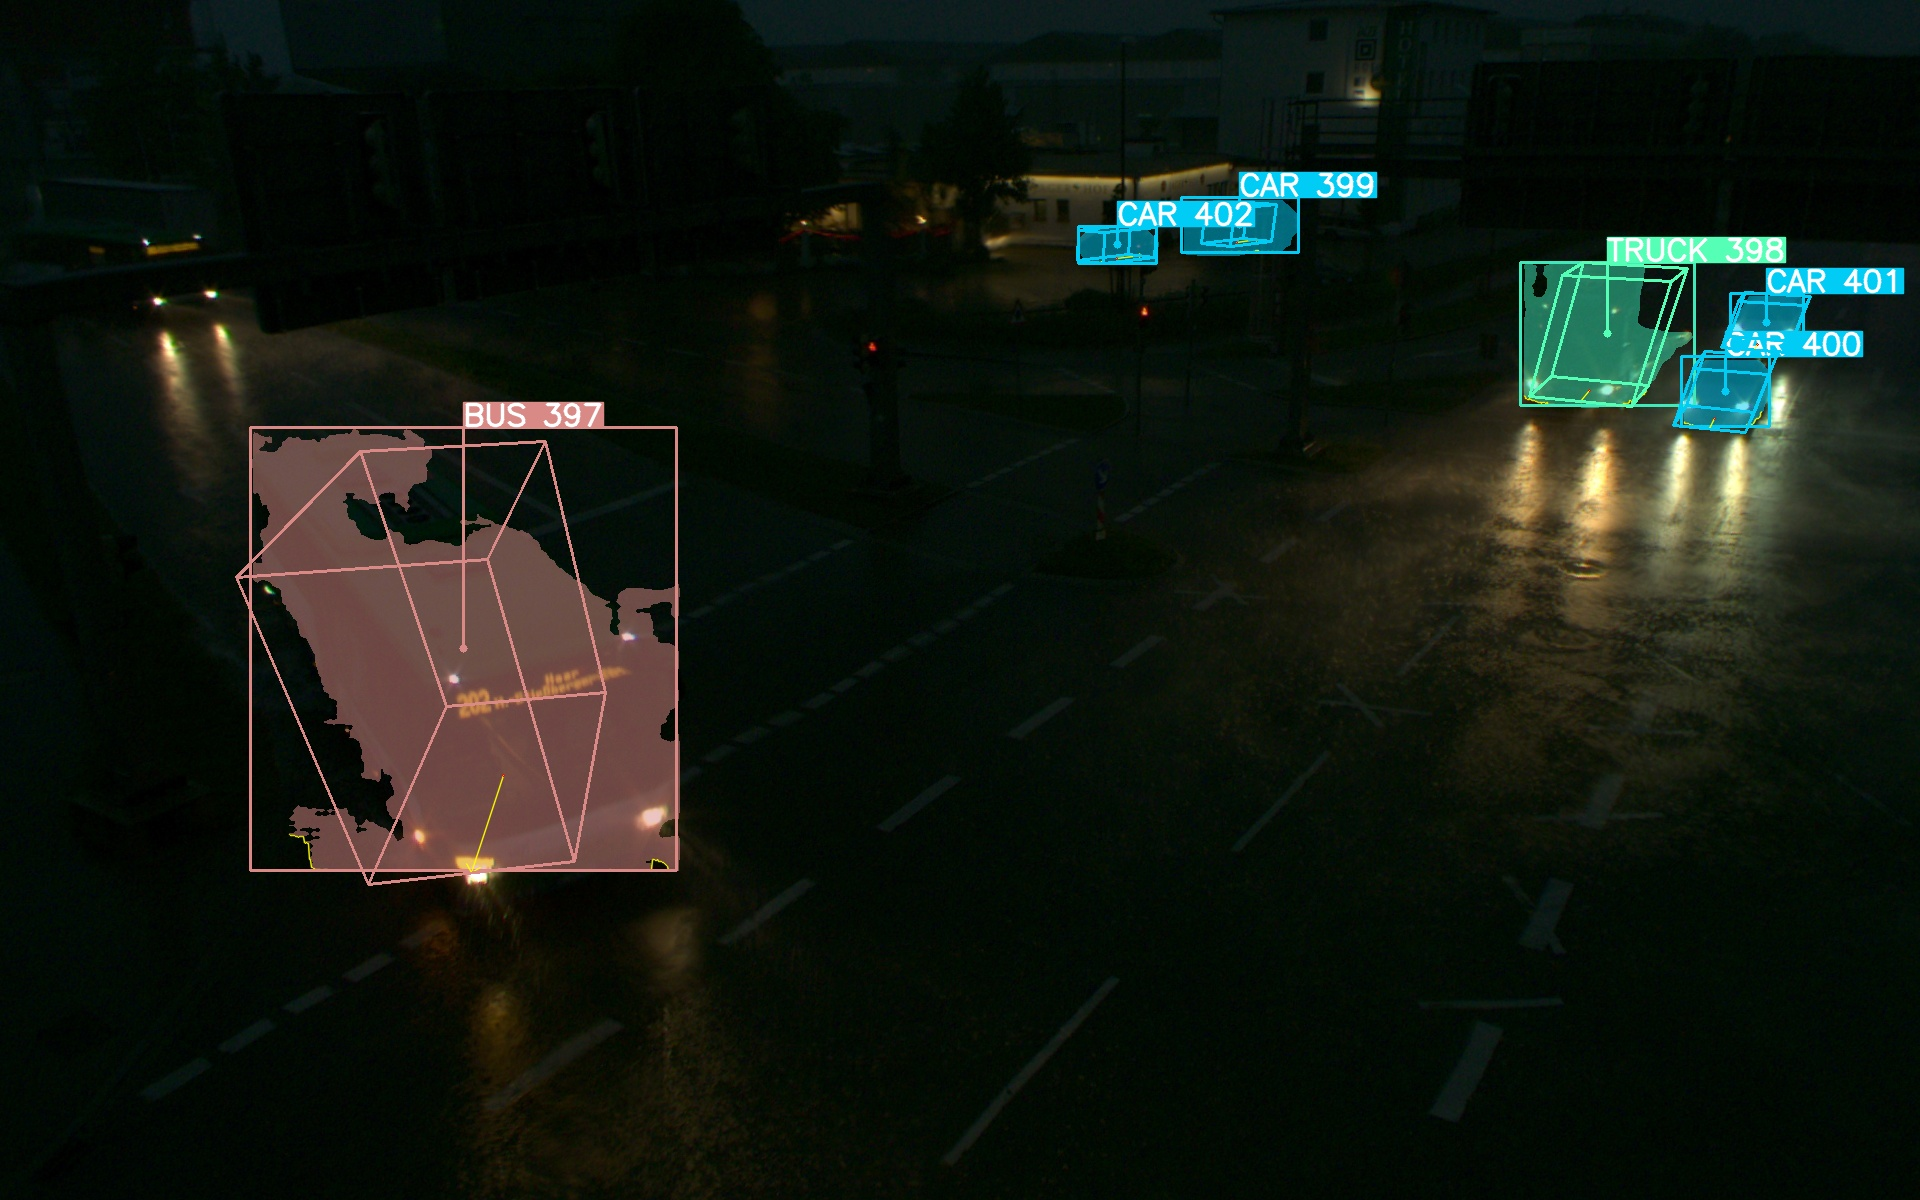
\includegraphics[width=\linewidth]{night_bus_yolov8_finetuned.jpg}
		\end{subfigure}\hfill
		\begin{subfigure}{0.245\textwidth}
			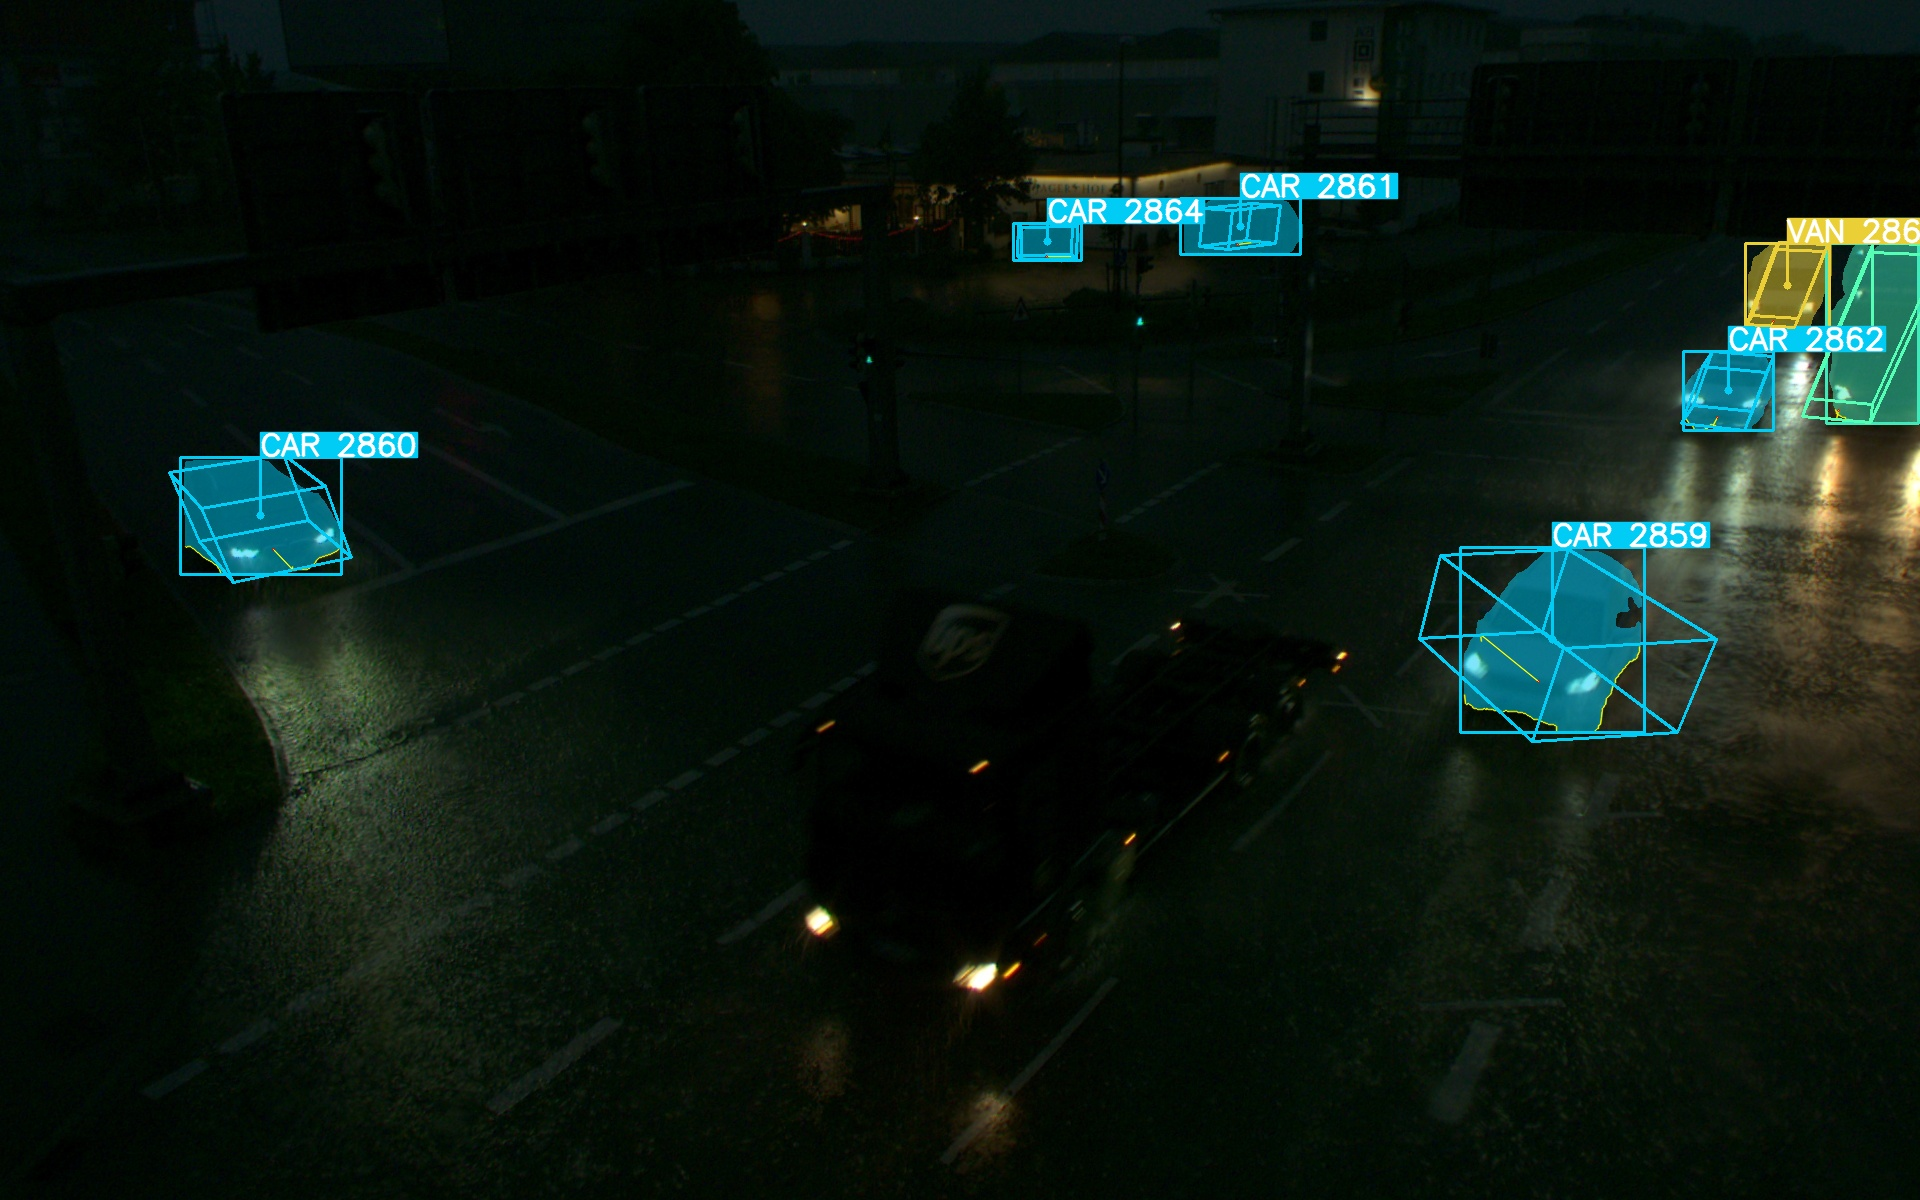
\includegraphics[width=\linewidth]{night_yolov8_finetuned.jpg}
		\end{subfigure}
		%\caption{\small $YOLOv8x\_coco\_tumtraf\_1920$}
	\end{subfigure}
	\captionof{figure}{ \textbf{Night sequence}: Qualitative comparisons of night sequence prediction of baseline detector $YOLOv7\_coco$ (first row) and the proposed detector with model weight $YOLOv8x\_tumtraf$ (second row) and with model weight $YOLOv8x\_coco\_tumtraf\_1920$ (third row).The visualizations include 2D bounding boxes, 2D masks, 3D bounding boxes, and category labels.}
	\label{figure:night_sequence}
	
\end{table}%

\begin{table}[htb]%
	\centering
	\scriptsize
	\setlength\tabcolsep{4pt}
	\hspace{-3em} % left shift
	\begin{minipage}{\textwidth}
		\begin{minipage}[t]{0.48\textwidth}
			\centering 
			$\bm{YOLOv7\_coco}$ (Baseline)\\
			\begin{tabular}{lrrr}
				\toprule
				\textbf{Classes} & \textbf{Precision} & \textbf{Recall} & \textbf{AP@[.10]} \\
				\midrule
				CAR & 26.85 & 9.92 & 20.21  \\
				TRUCK & 0.46 & 0.07 & 0.26  \\
				VAN & 0.00 & 0.00 & 0.00  \\
				BUS & 22.58 & 8.85 & 19.68  \\
				\midrule
				\textbf{mAP@[.10]} & \textbf{} & \textbf{} & \textbf{8.03}   \\
				\bottomrule
			\end{tabular}
		\end{minipage}%
		\hfill
		\begin{minipage}[t]{0.48\textwidth}
			\centering 
			$\bm{YOLOv8x\_tumtraf}$\\
			\begin{tabular}{lrrrr}
				\toprule
				\textbf{Classes} & \textbf{Precision} & \textbf{Recall} & \textbf{AP@[.10]} & \textbf{$\triangle$Baseline} \\
				\midrule
				CAR & 34.26 & 14.13 & 28.16 &  \textcolor{darkgreen}{+ 7.95}\\
				TRUCK & 4.68 & 4.56 & 3.86 &  \textcolor{darkgreen}{+ 3.60}\\
				VAN & 22.33 & 17.45 & 20.97 & \textcolor{darkgreen}{+ 20.97}\\
				BUS & 40.88 & 29.24 & 38.30 & \textcolor{darkgreen}{+ 18.62}\\
				\midrule
				\textbf{mAP@[.10]} & \textbf{} & \textbf{} & \textbf{18.26}   & \textbf{\textcolor{darkgreen}{+ 10.23}} \\
				\bottomrule
			\end{tabular}
		\end{minipage}
	\end{minipage}
	
	\vspace{2em} % space between two tables
	\begin{minipage}[t]{0.48\textwidth}
		\centering 
		$\bm{YOLOv8x\_coco\_tumtraf\_1920}$\\
		\begin{tabular}{lrrrr}
			\toprule
			\textbf{Classes} & \textbf{Precision} & \textbf{Recall} & \textbf{AP@[.10]} & \textbf{$\triangle$Baseline} \\
			\midrule
			CAR & 27.16 & 12.34 & 21.05 &  \textcolor{darkgreen}{+ 0.84}\\
			TRUCK & 4.18 & 3.94 & 3.45 &  \textcolor{darkgreen}{+ 3.19}\\
			VAN & 10.59 & 5.475 & 8.59 &  \textcolor{darkgreen}{+ 8.59}\\
			BUS & 18.23 & 13.98 & 16.21 &  \textcolor{darkred}{- 3.47}\\
			\midrule
			\textbf{mAP@[.10]} & \textbf{} & \textbf{} & \textbf{9.86}   & \textbf{\textcolor{darkgreen}{+ 1.83}} \\
			\bottomrule
		\end{tabular}
	\end{minipage}
	
	\captionof{table}{\textbf{Night sequence}: 3D detection quantitative comparisons on the night sequence.}
	\label{tab:night_sequence}
\end{table}

\Cref{tab:night_sequence} and \Cref{figure:night_sequence} demonstrate the results on the night scenario sequence (S04) of the TUMTraf Intersection Dataset. The model trained from scratch on the TUMTraf Intersection Dataset achieves a notable performance enhancement, surpassing the existing 2D detector based on YOLOv7 by over 10\%. Conversely, the model pre-trained on COCO and subsequently fine-tuned on the TUMTraf Intersection Dataset exhibits a modest improvement of 1.83\%. Additionally, the performance of the YOLOv8x\_coco pre-trained weight from Ultralytics is also assessed, showing an improvement of only 0.57\% over the baseline.

The qualitative results demonstrate that the YOLOv8 models provide more stable predictions compared to the baseline YOLOv7. While YOLOv7 can identify vehicles, its predictions are unstable as objects can sometimes be identified and sometimes not. In contrast, YOLOv8 can predict objects with stability throughout the sequence, as illustrated in the first two frames.

YOLOv8x\_coco\_tumtraf\_1920 has stable detections but performs notably worse than the YOLOv8x\_tumtraf model. It exhibits buggy predicted object masks (frame 3 of the third row), with several objects remaining undetected (frames 1 and 2 of the third row).

Remarkably, YOLOv8x\_tumtraf outperforms others in the night sequence of the TUMTraf Intersection Dataset, offering stable predictions and significantly improved identification of large vehicles.

\section{Performance on TUMTraf Intersection Dataset} \label{sec:ablation_study_intersection}

\begin{table}[htb]%
	\centering
	\begin{tabular}[htb]{lrrrrrr}
		\toprule
		\textbf{Model} & \textbf{S01} & \textbf{S02} & \textbf{S03} & \textbf{S04} & \textbf{Average} & \textbf{$\triangle$Baseline} \\
		\midrule
		$YOLOv7\_coco$ (Baseline) & 23.91 & 15.79 & 11.87 & 8.03 & 12.91 \\
		$YOLOv8x\_coco$ & 20.60 & 13.82 & 12.01 & 8.60 & 15.20 & \textcolor{darkgreen}{+ 2.29}  \\
		$YOLOv8x\_tumtraf$ & \underline{\textbf{41.27}} & \textbf{17.48} & \textbf{17.50} & \underline{\textbf{18.26}} & \underline{\textbf{20.66}} & \textcolor{darkgreen}{+ 7.75}  \\
		$YOLOv8x\_coco\_tumtraf\_1920$ & \textbf{32.42} & \underline{\textbf{17.91}} & \underline{\textbf{21.03}} & \textbf{9.86} & \textbf{19.27} & \textcolor{darkgreen}{+ 6.36}  \\
		\midrule
	\end{tabular}
	\caption{\textbf{Entire TUMTraf Intersection Dataset}: 3D mAP@[.10] comparisons across all sequences of the TUMTraf Intersection Dataset. Sequence 03 constitutes the largest portion of the TUMTraf Intersection Dataset, accounting for 50\% of the dataset with 2400 frames, followed by the night sequence 04, analyzed previously, with 1200 frames (25\%). Sequences 01 and 02 each contain 600 frames, collectively representing the remaining 25\%. Thus, the average mAP values are weighted based on a ratio of 1:1:4:2 for sequences 01 to 04, respectively. This weighting ensures a fair representation of each sequence's contribution to the overall performance evaluation.}
	\label{tab:ablation_study_intersection}
\end{table}

\Cref{tab:ablation_study_intersection} presents the 3D mean Average Precision comparison of the YOLOv8 model weights with the baseline model YOLOv7 across all sequences of the TUMTraf Intersection Dataset. Once more, the model weight YOLOv8x\_tumtraf showcases the most significant performance improvement. The improvement percentages are not very different from the 3D quantitative analysis of the test sequence alone in \Cref{sec:quan_3d}.

\section{Performance on Highway} \label{sec:ablation_study_highway}

\begin{table}[htb]%
	\centering
	\small
	\setlength\tabcolsep{4pt}
	
	\begin{subfigure}{\textwidth}
		\centering
		\begin{subfigure}{0.32\textwidth}
			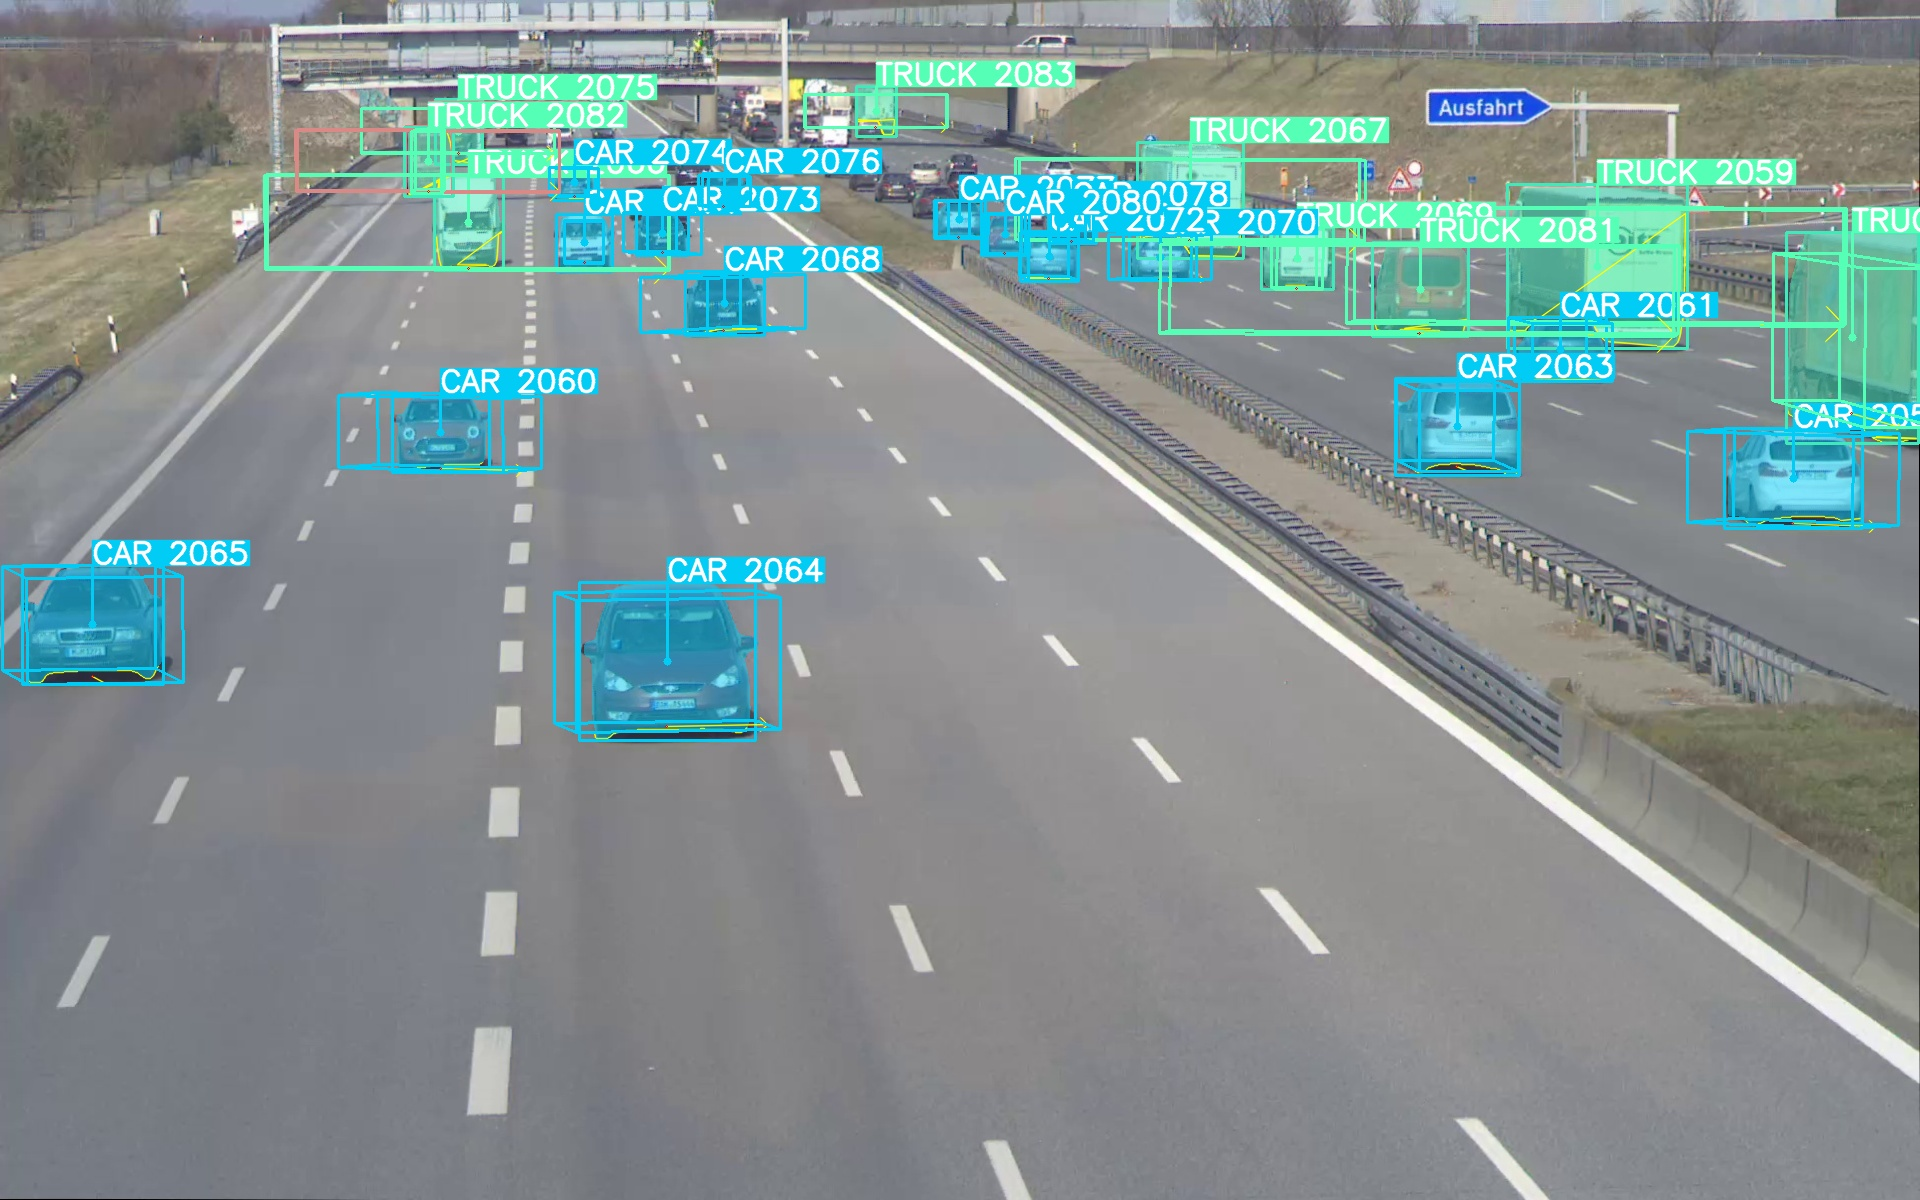
\includegraphics[width=\linewidth]{1616762544_288000000_yolov7.jpg}
		\end{subfigure}\hfill
		\begin{subfigure}{0.32\textwidth}
			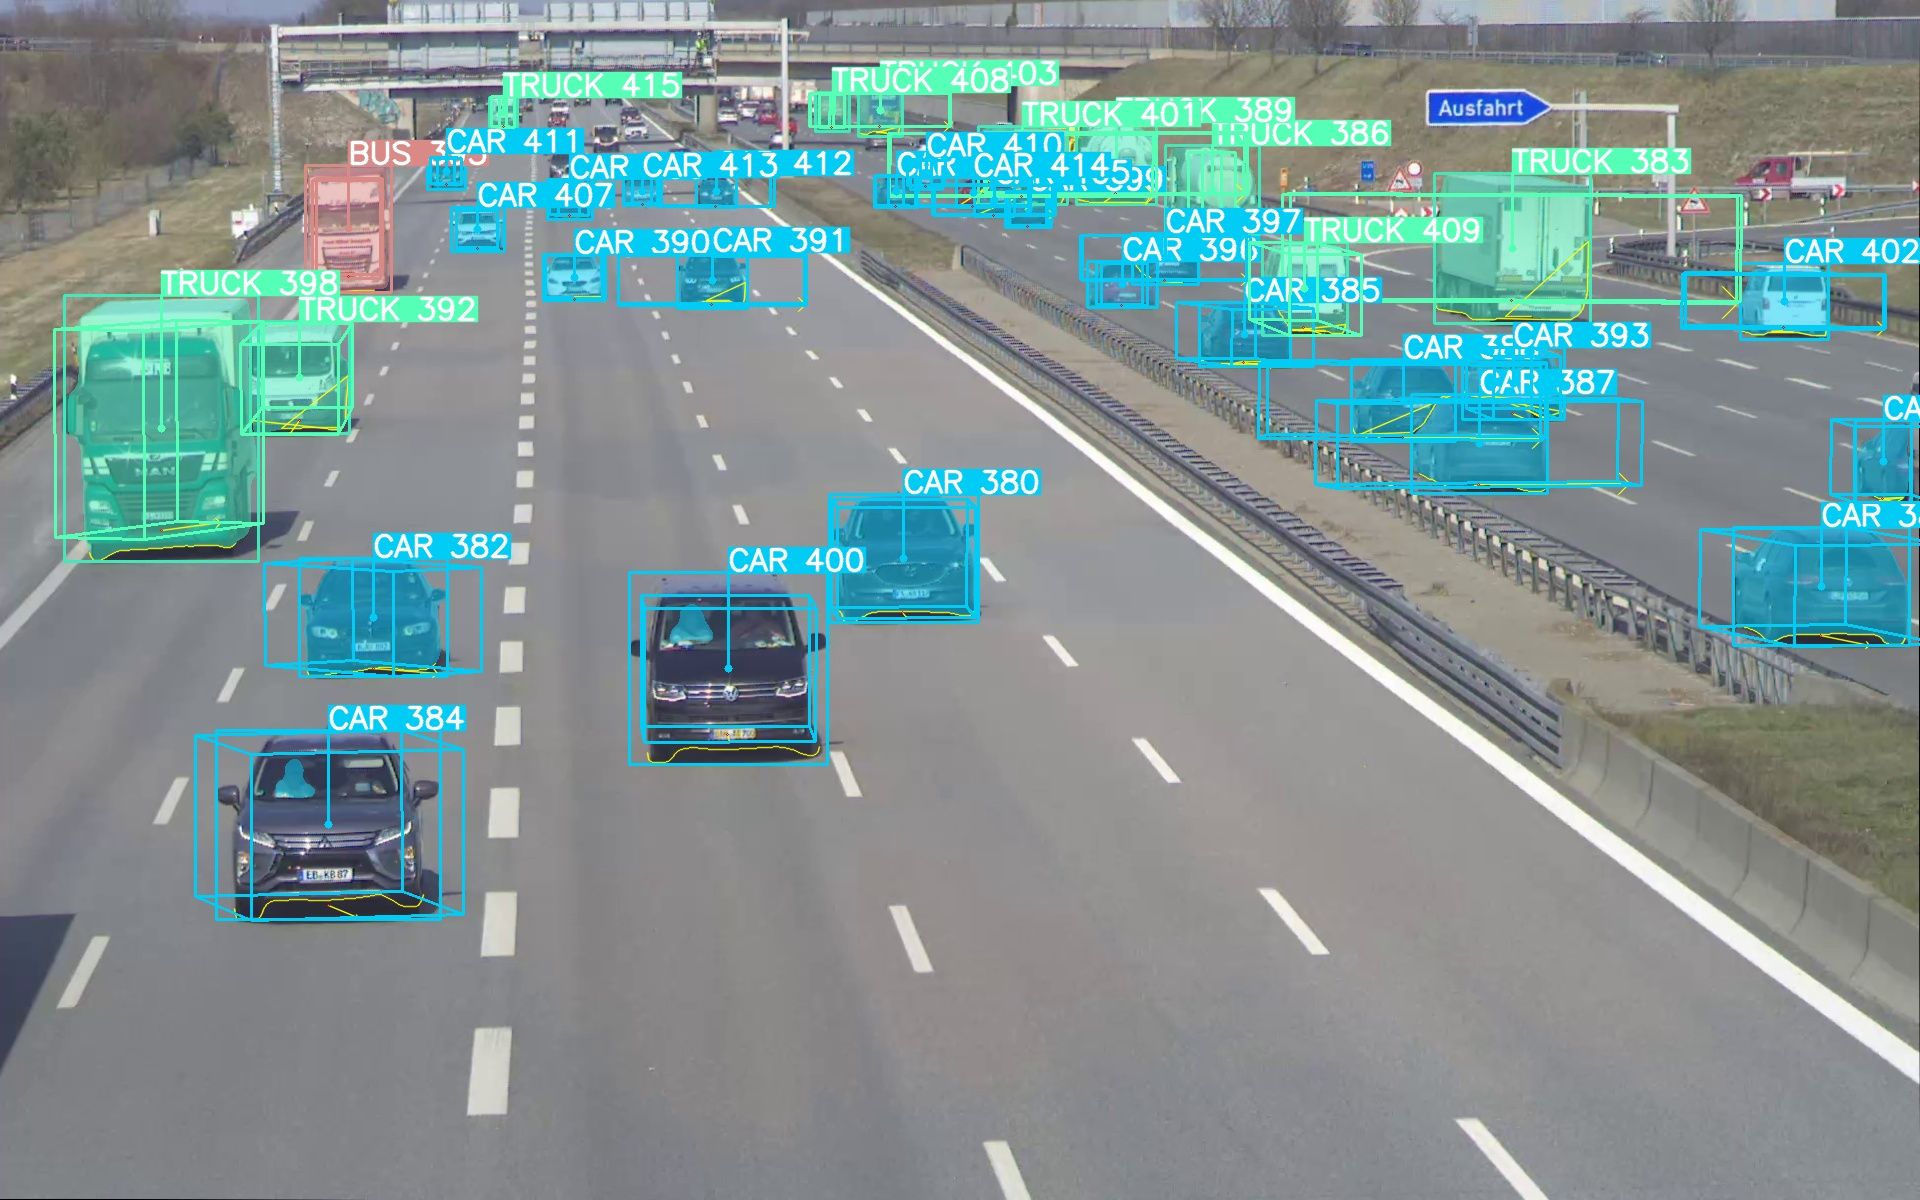
\includegraphics[width=\linewidth]{1616762525_089000000_yolov7.jpg}
		\end{subfigure}\hfill
		\begin{subfigure}{0.32\textwidth}
			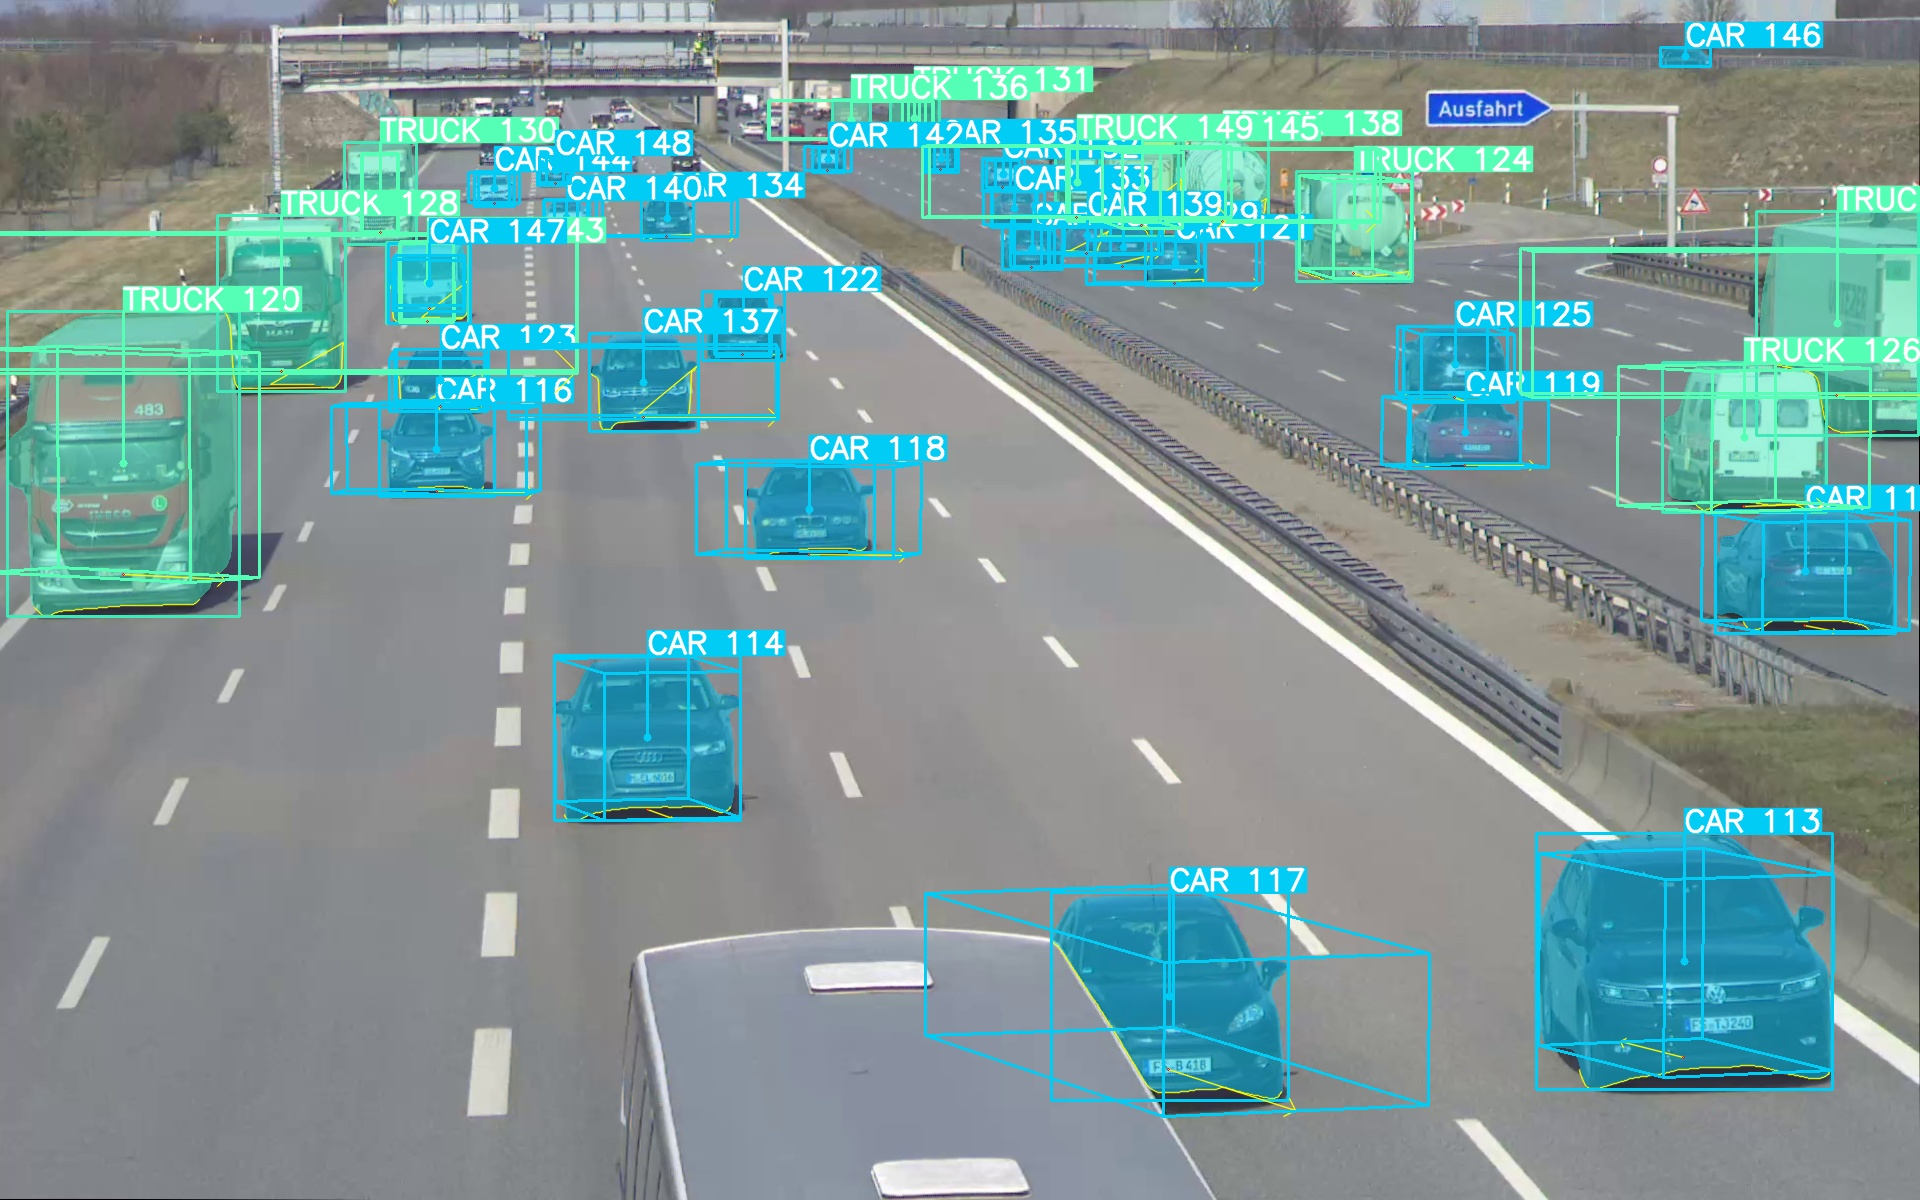
\includegraphics[width=\linewidth]{1616762522_288000000_yolov7.jpg}
		\end{subfigure}
		%\caption{\small $YOLOv7\_coco$}
	\end{subfigure}
	
	\begin{subfigure}{\textwidth}
		\centering
		\begin{subfigure}{0.32\textwidth}
			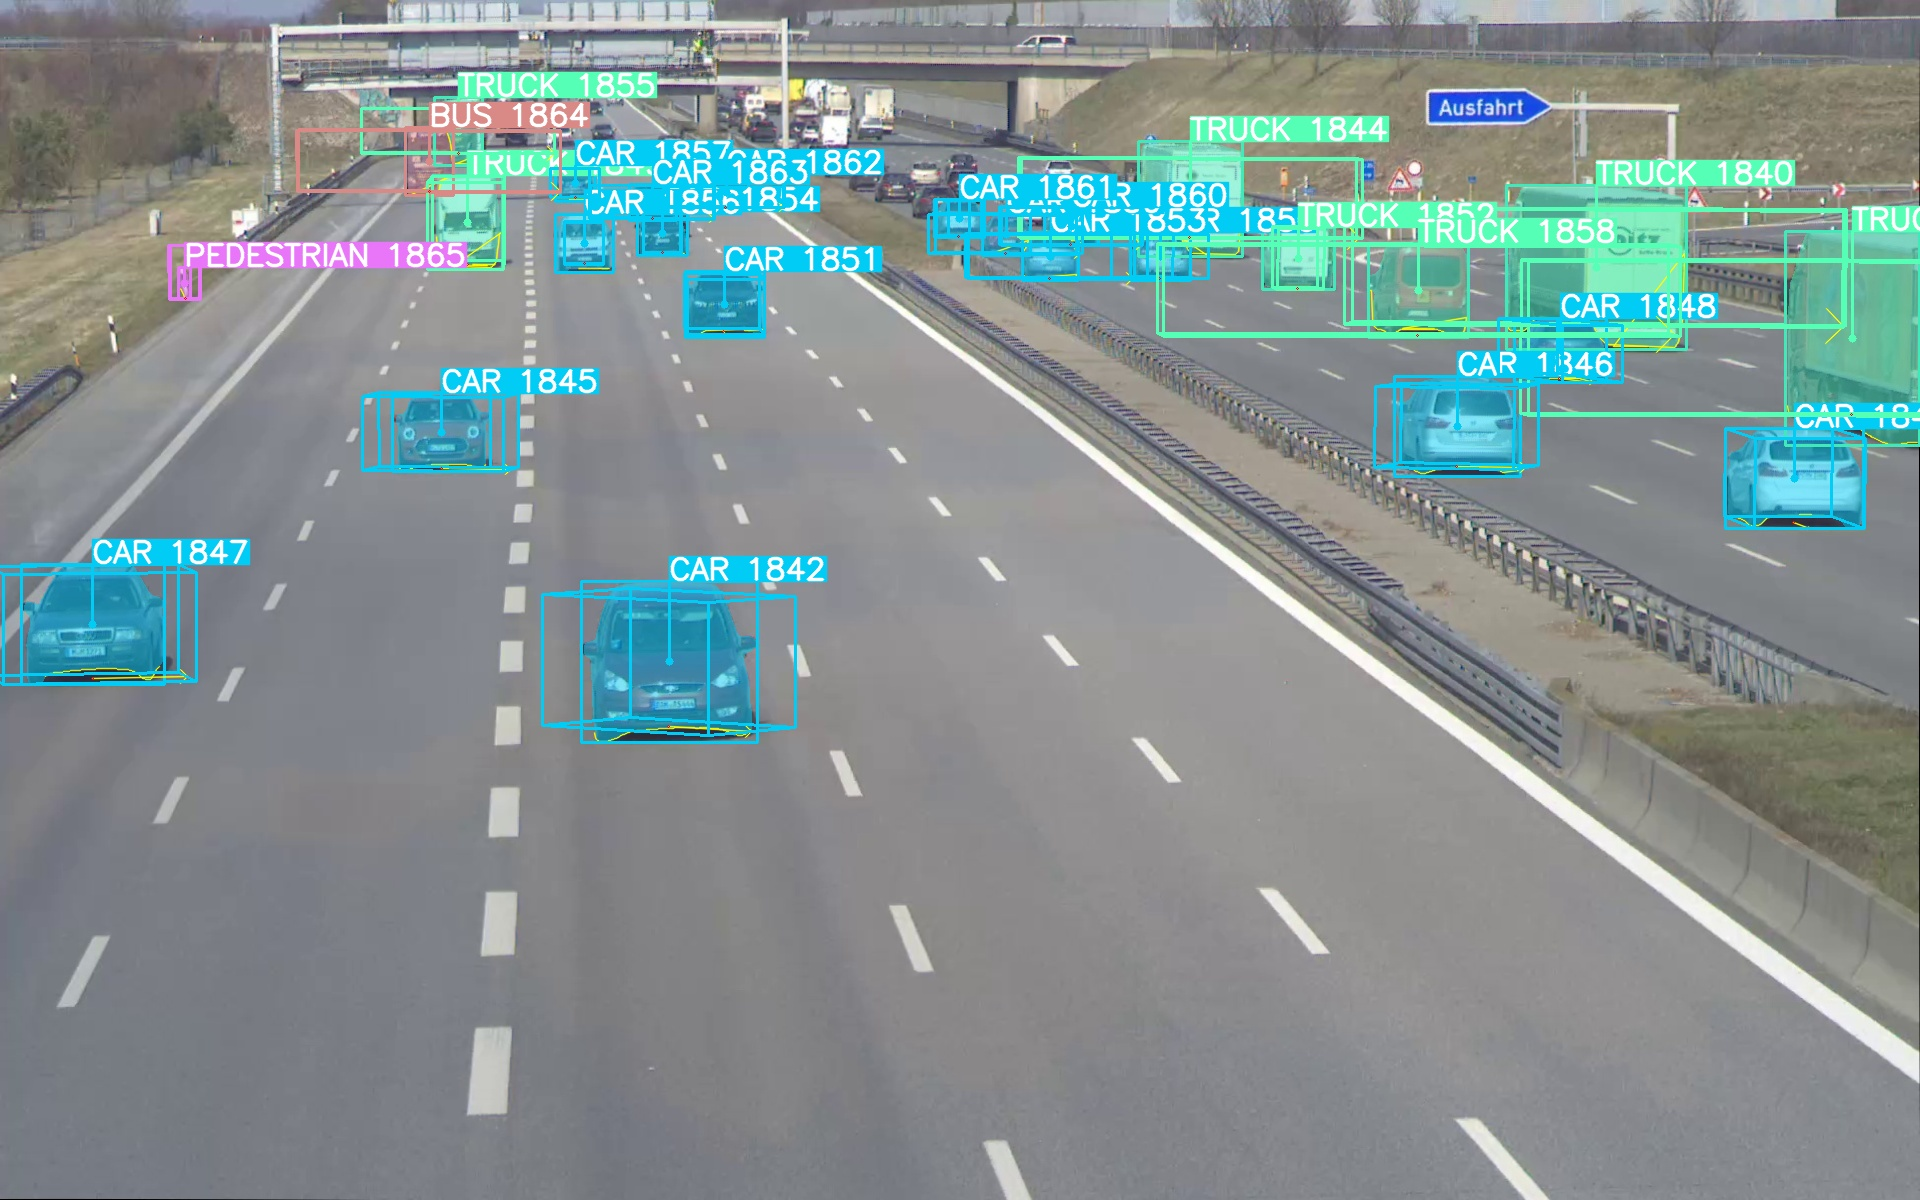
\includegraphics[width=\linewidth]{1616762544_288000000_yolov8.jpg}
		\end{subfigure}\hfill
		\begin{subfigure}{0.32\textwidth}
			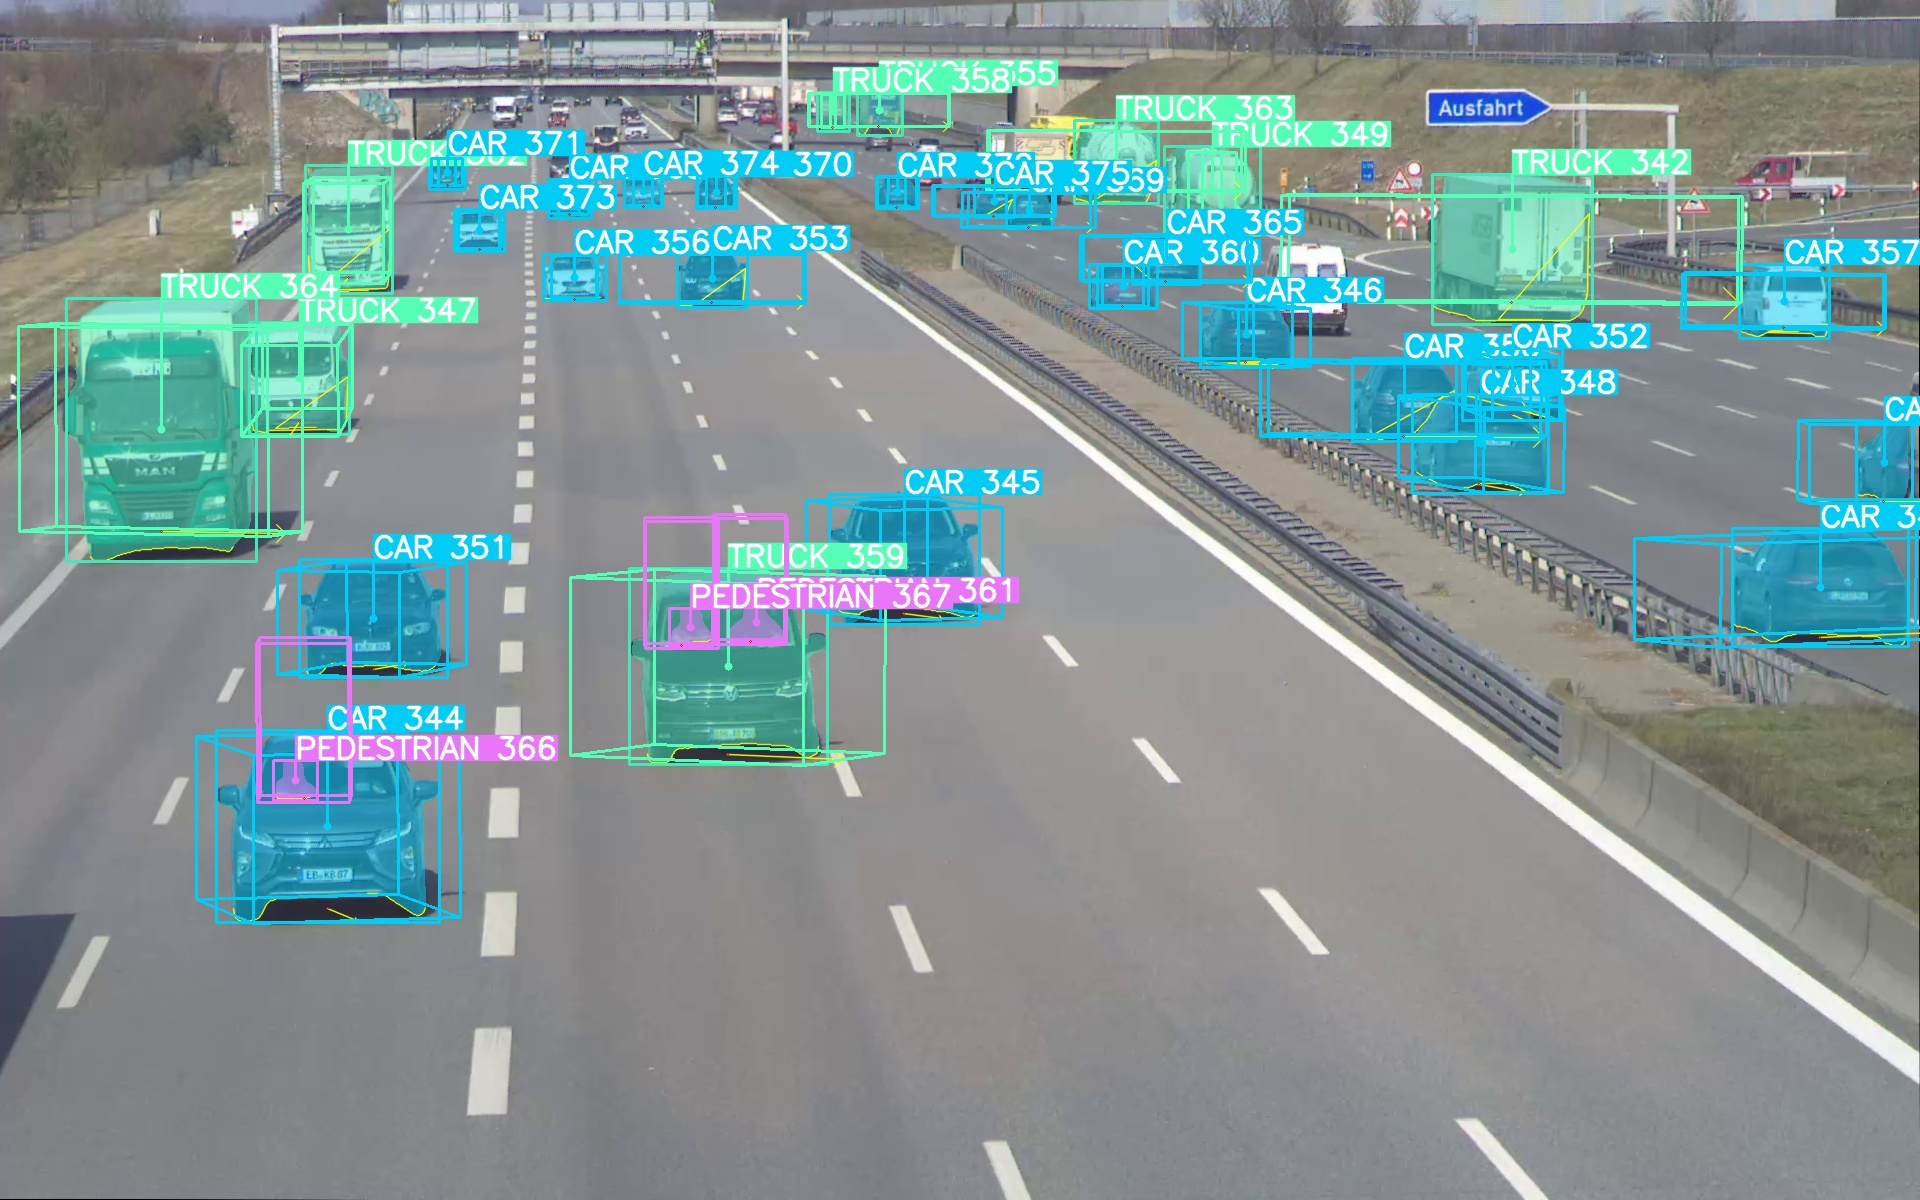
\includegraphics[width=\linewidth]{1616762525_089000000_yolov8.jpg}
		\end{subfigure}\hfill
		\begin{subfigure}{0.32\textwidth}
			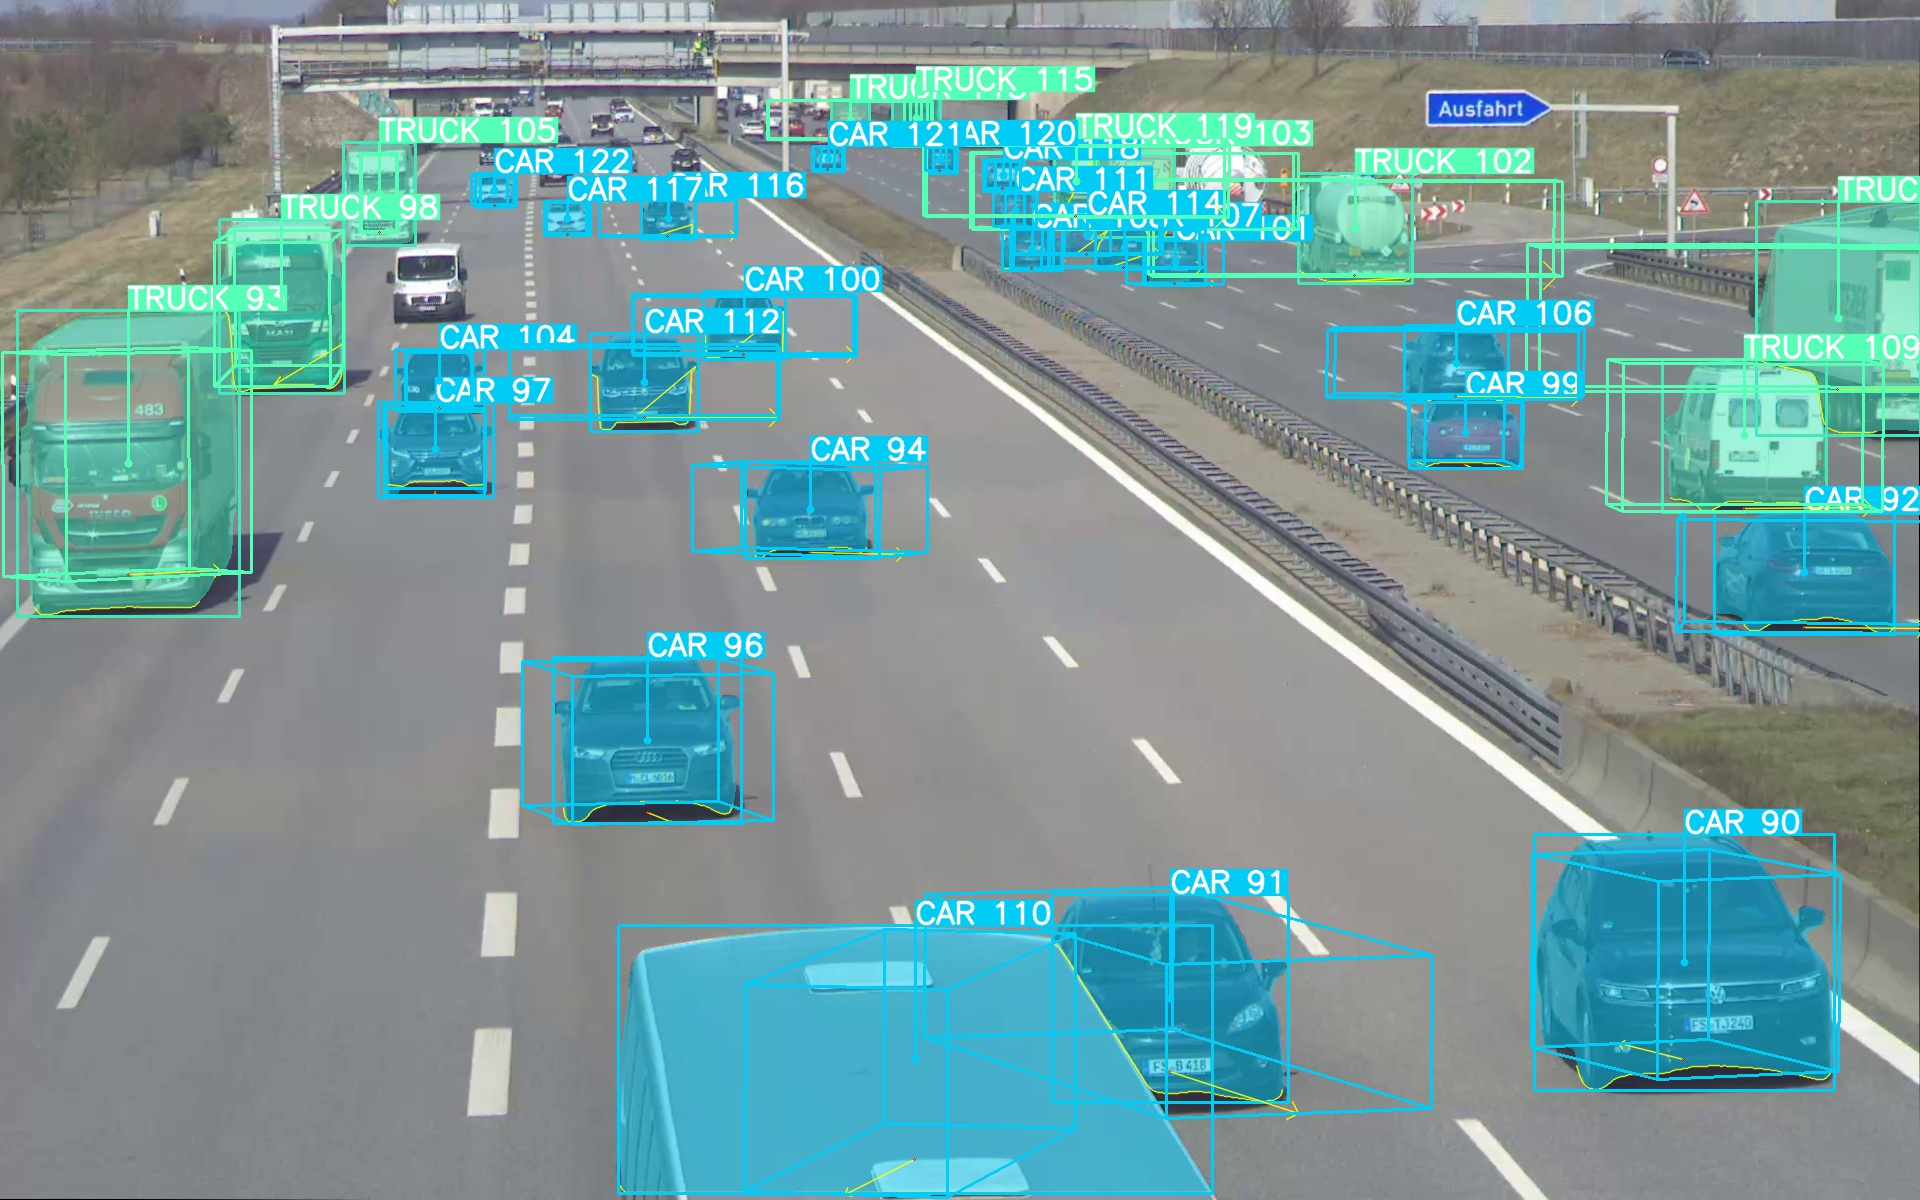
\includegraphics[width=\linewidth]{1616762522_288000000_yolov8.jpg}
		\end{subfigure}
		%\caption{\small $YOLOv8\_coco$}
	\end{subfigure}
	
	\begin{subfigure}{\textwidth}
		\centering
		\begin{subfigure}{0.32\textwidth}
			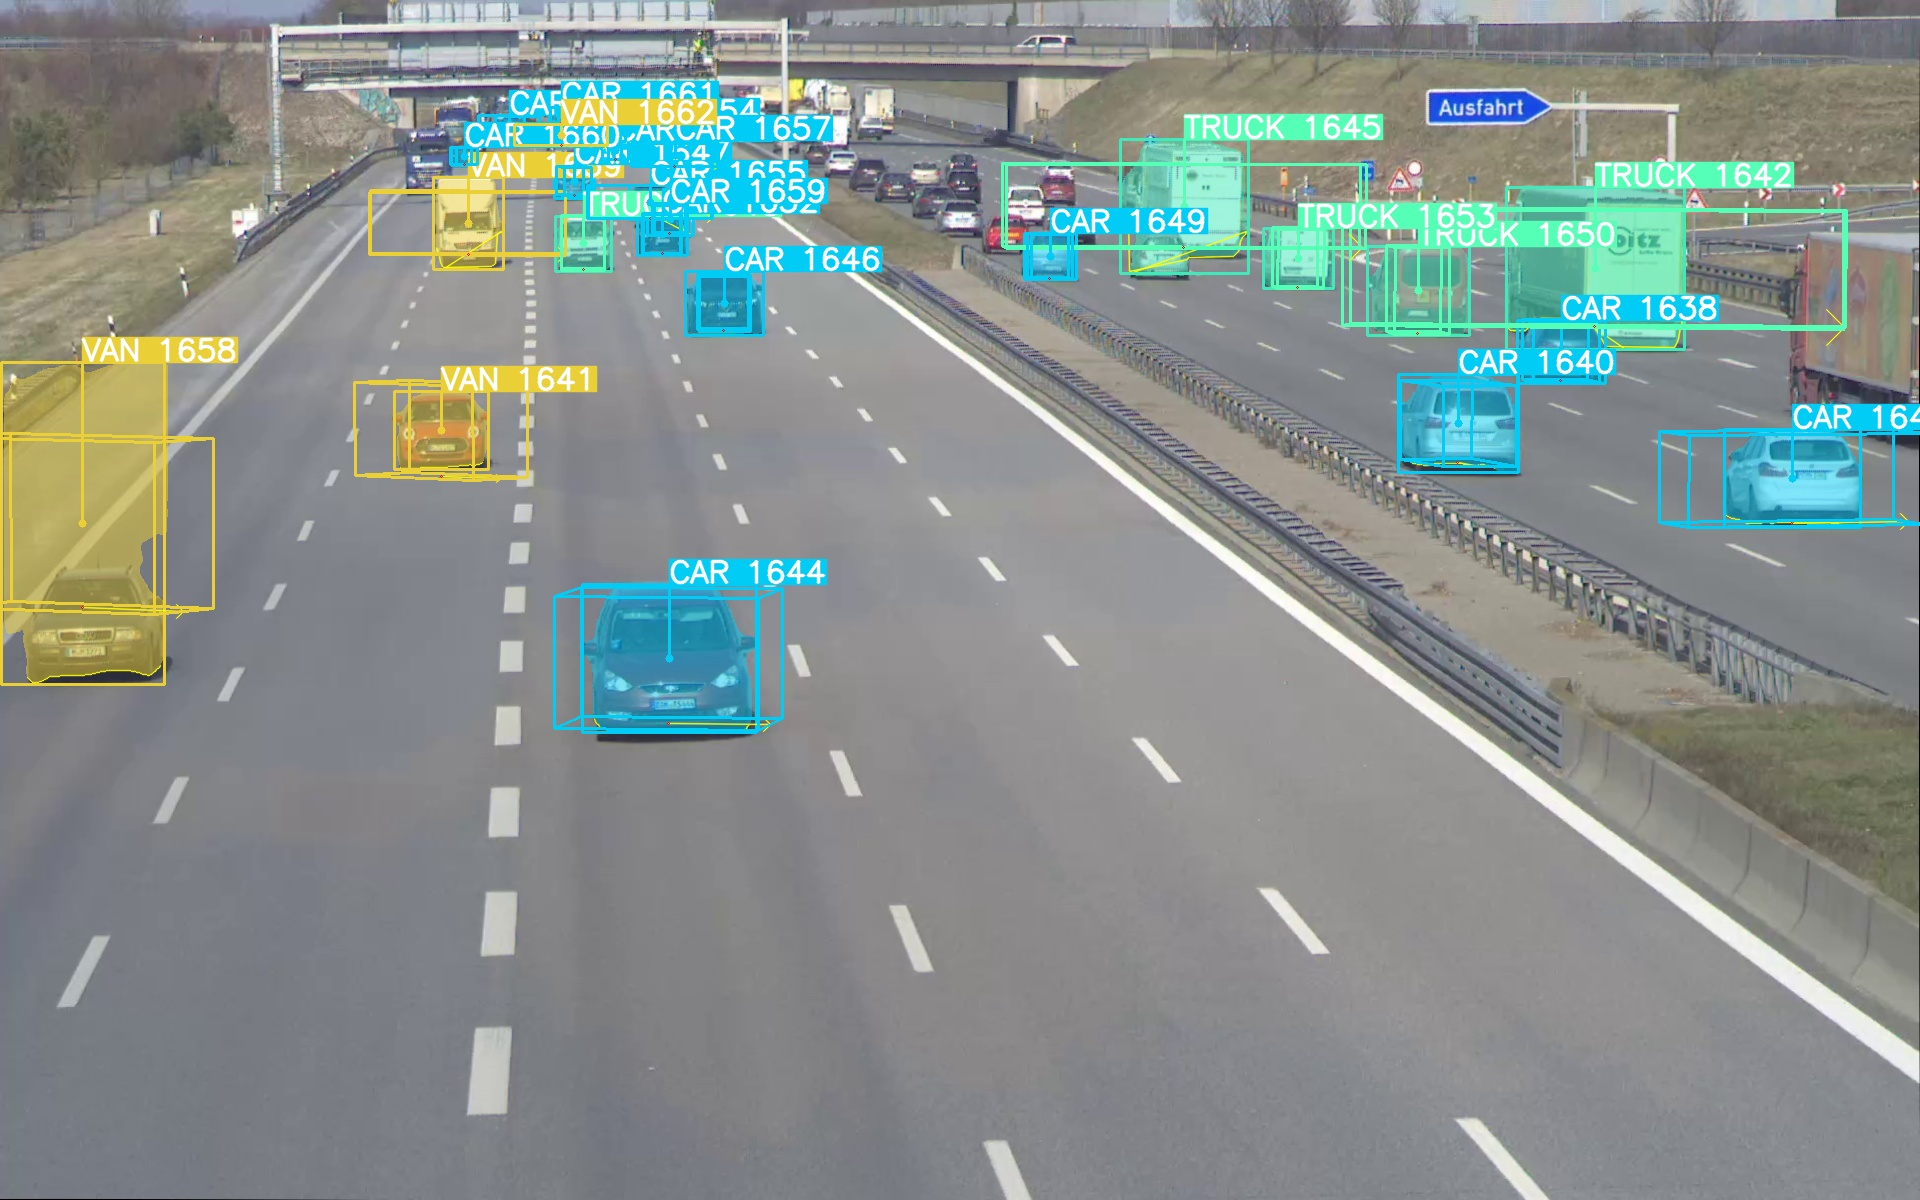
\includegraphics[width=\linewidth]{1616762544_288000000_scratch.jpg}
		\end{subfigure}\hfill
		\begin{subfigure}{0.32\textwidth}
			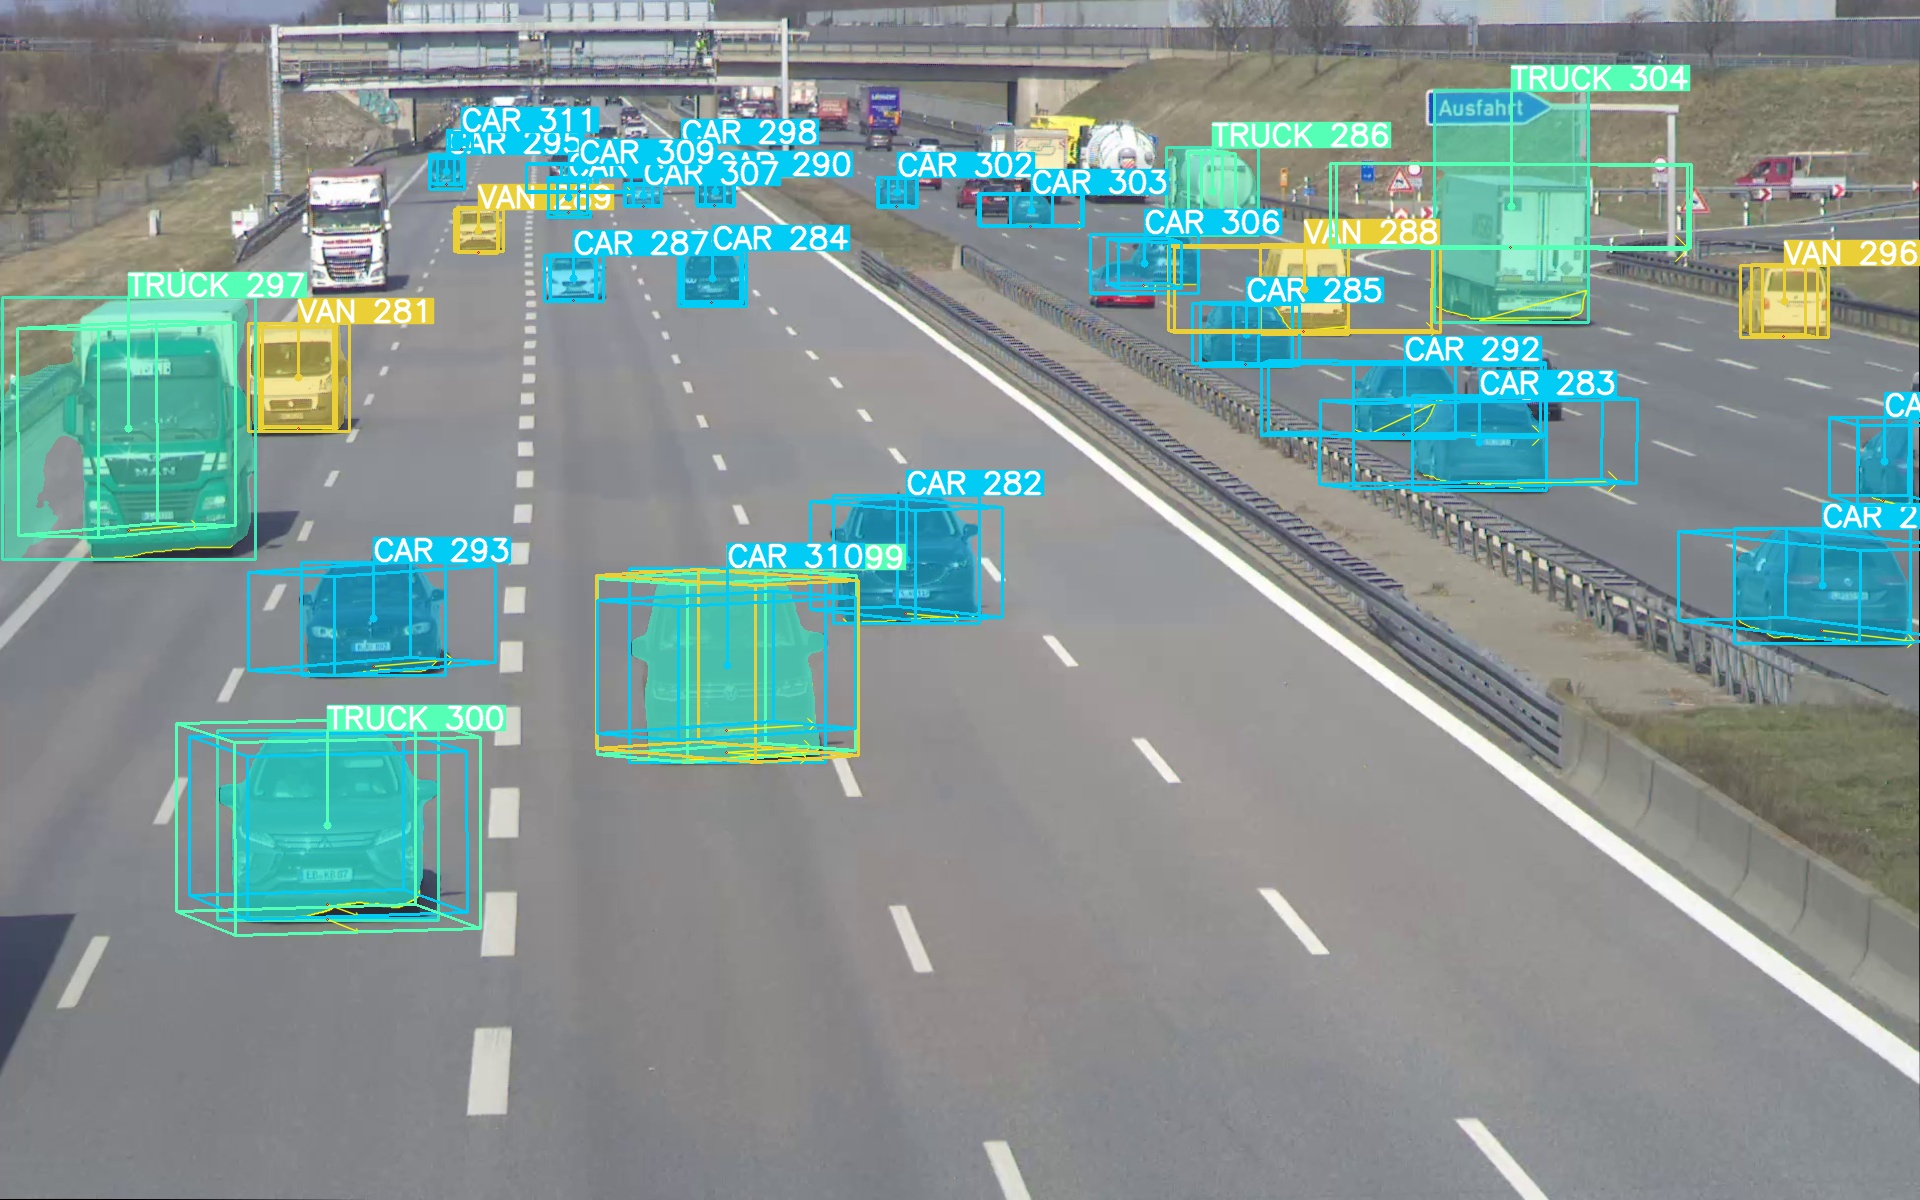
\includegraphics[width=\linewidth]{1616762525_089000000_scratch.jpg}
		\end{subfigure}\hfill
		\begin{subfigure}{0.32\textwidth}
			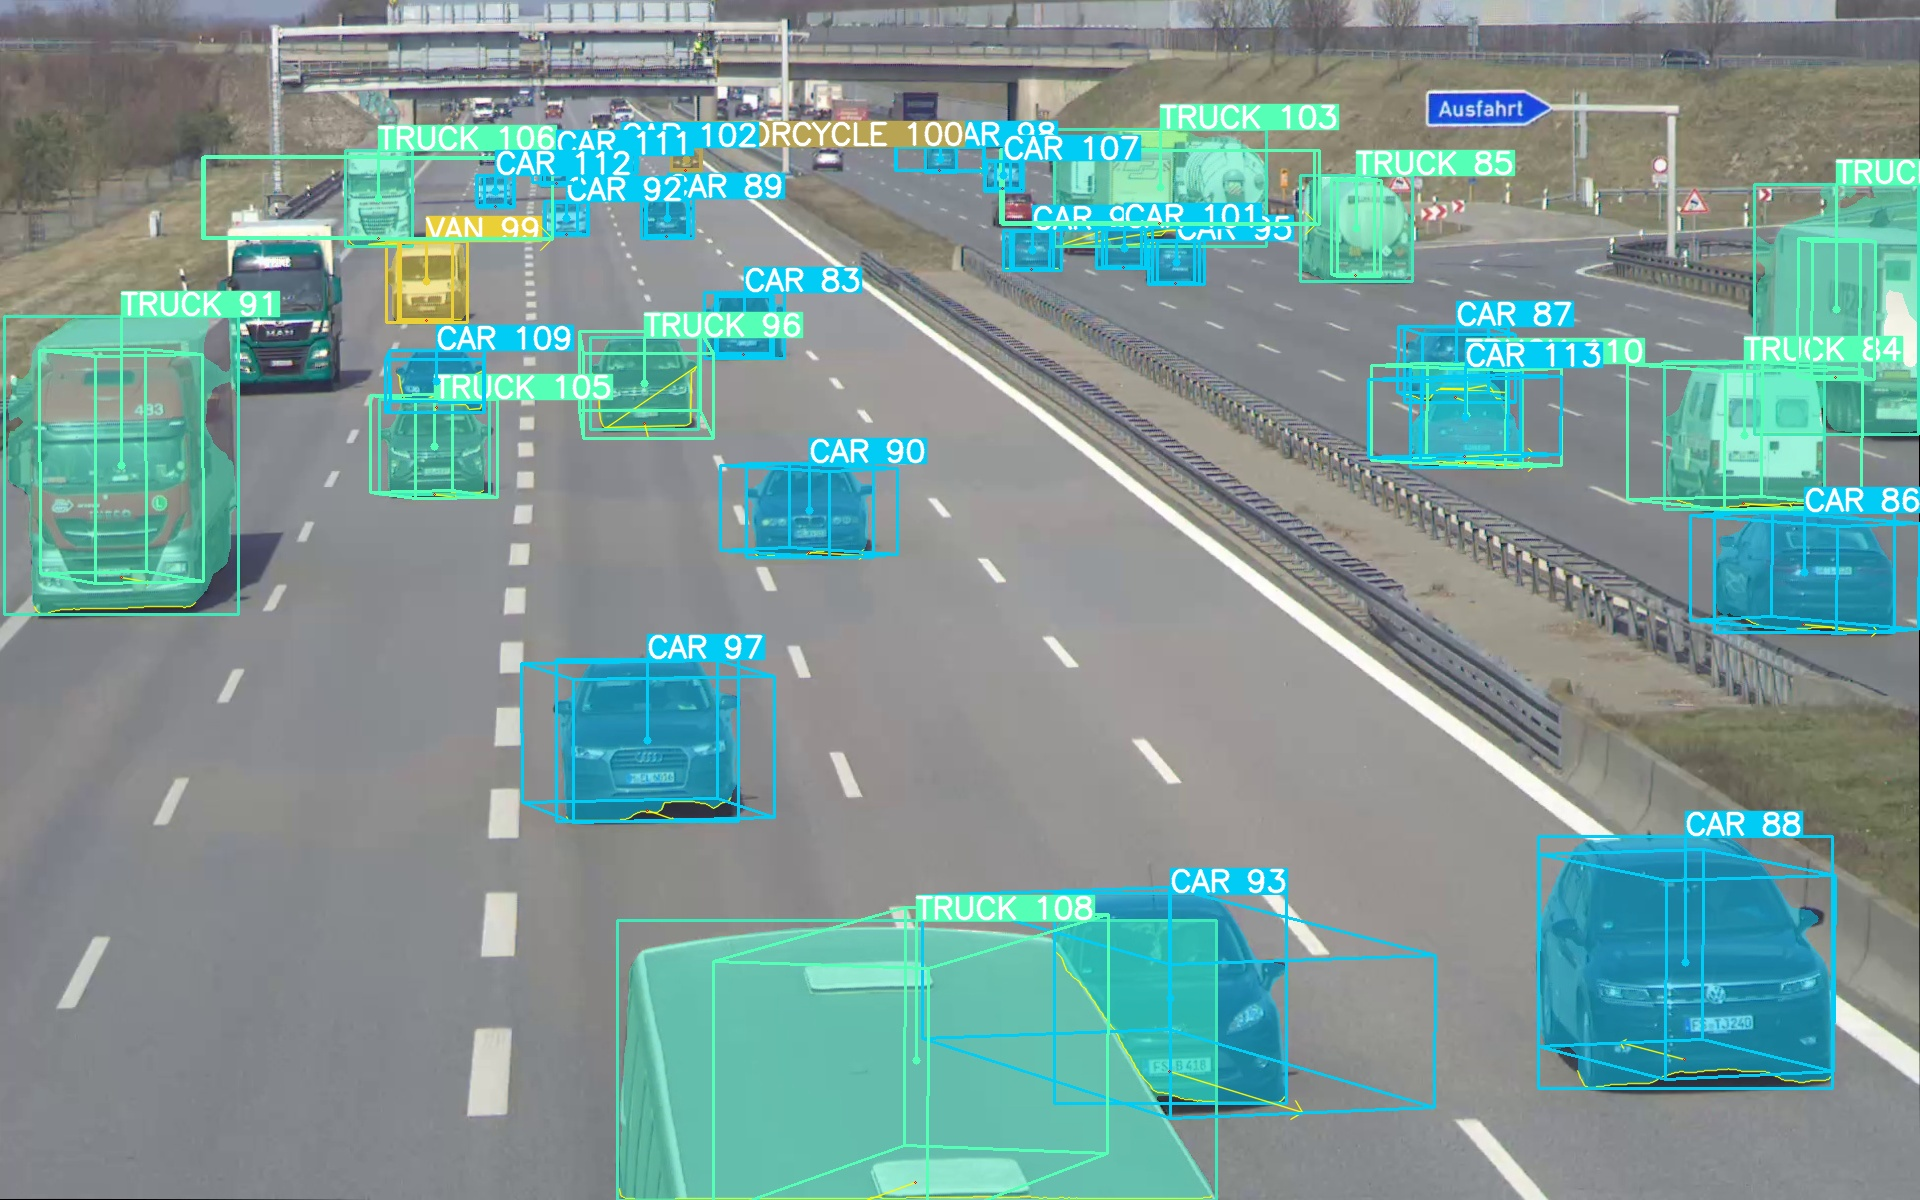
\includegraphics[width=\linewidth]{1616762522_288000000_scratch.jpg}
		\end{subfigure}
		%\caption{\small $YOLOv8x\_tumtraf$}
	\end{subfigure}
	
	\begin{subfigure}{\textwidth}
		\centering
		\begin{subfigure}{0.32\textwidth}
			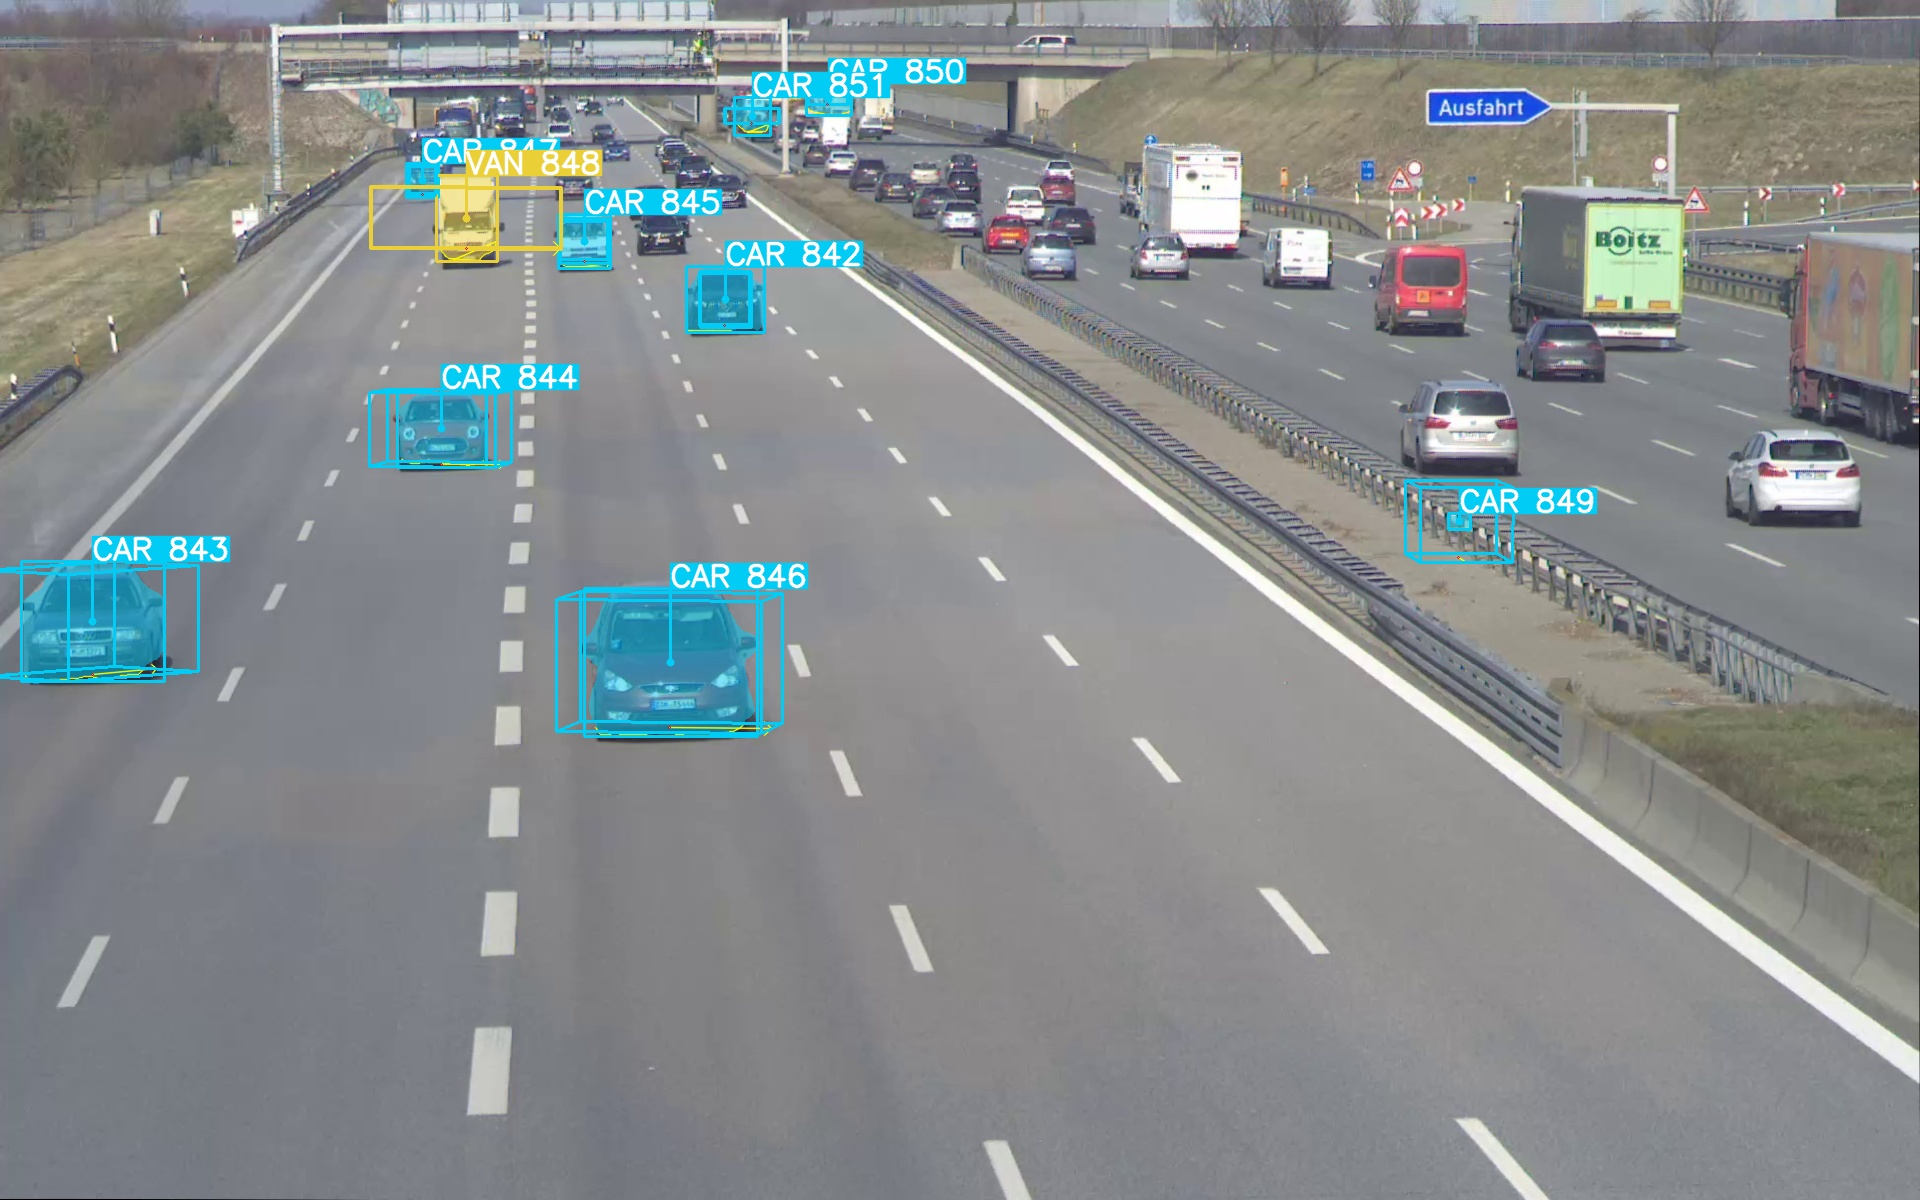
\includegraphics[width=\linewidth]{1616762544_288000000_finetuned.jpg}
		\end{subfigure}\hfill
		\begin{subfigure}{0.32\textwidth}
			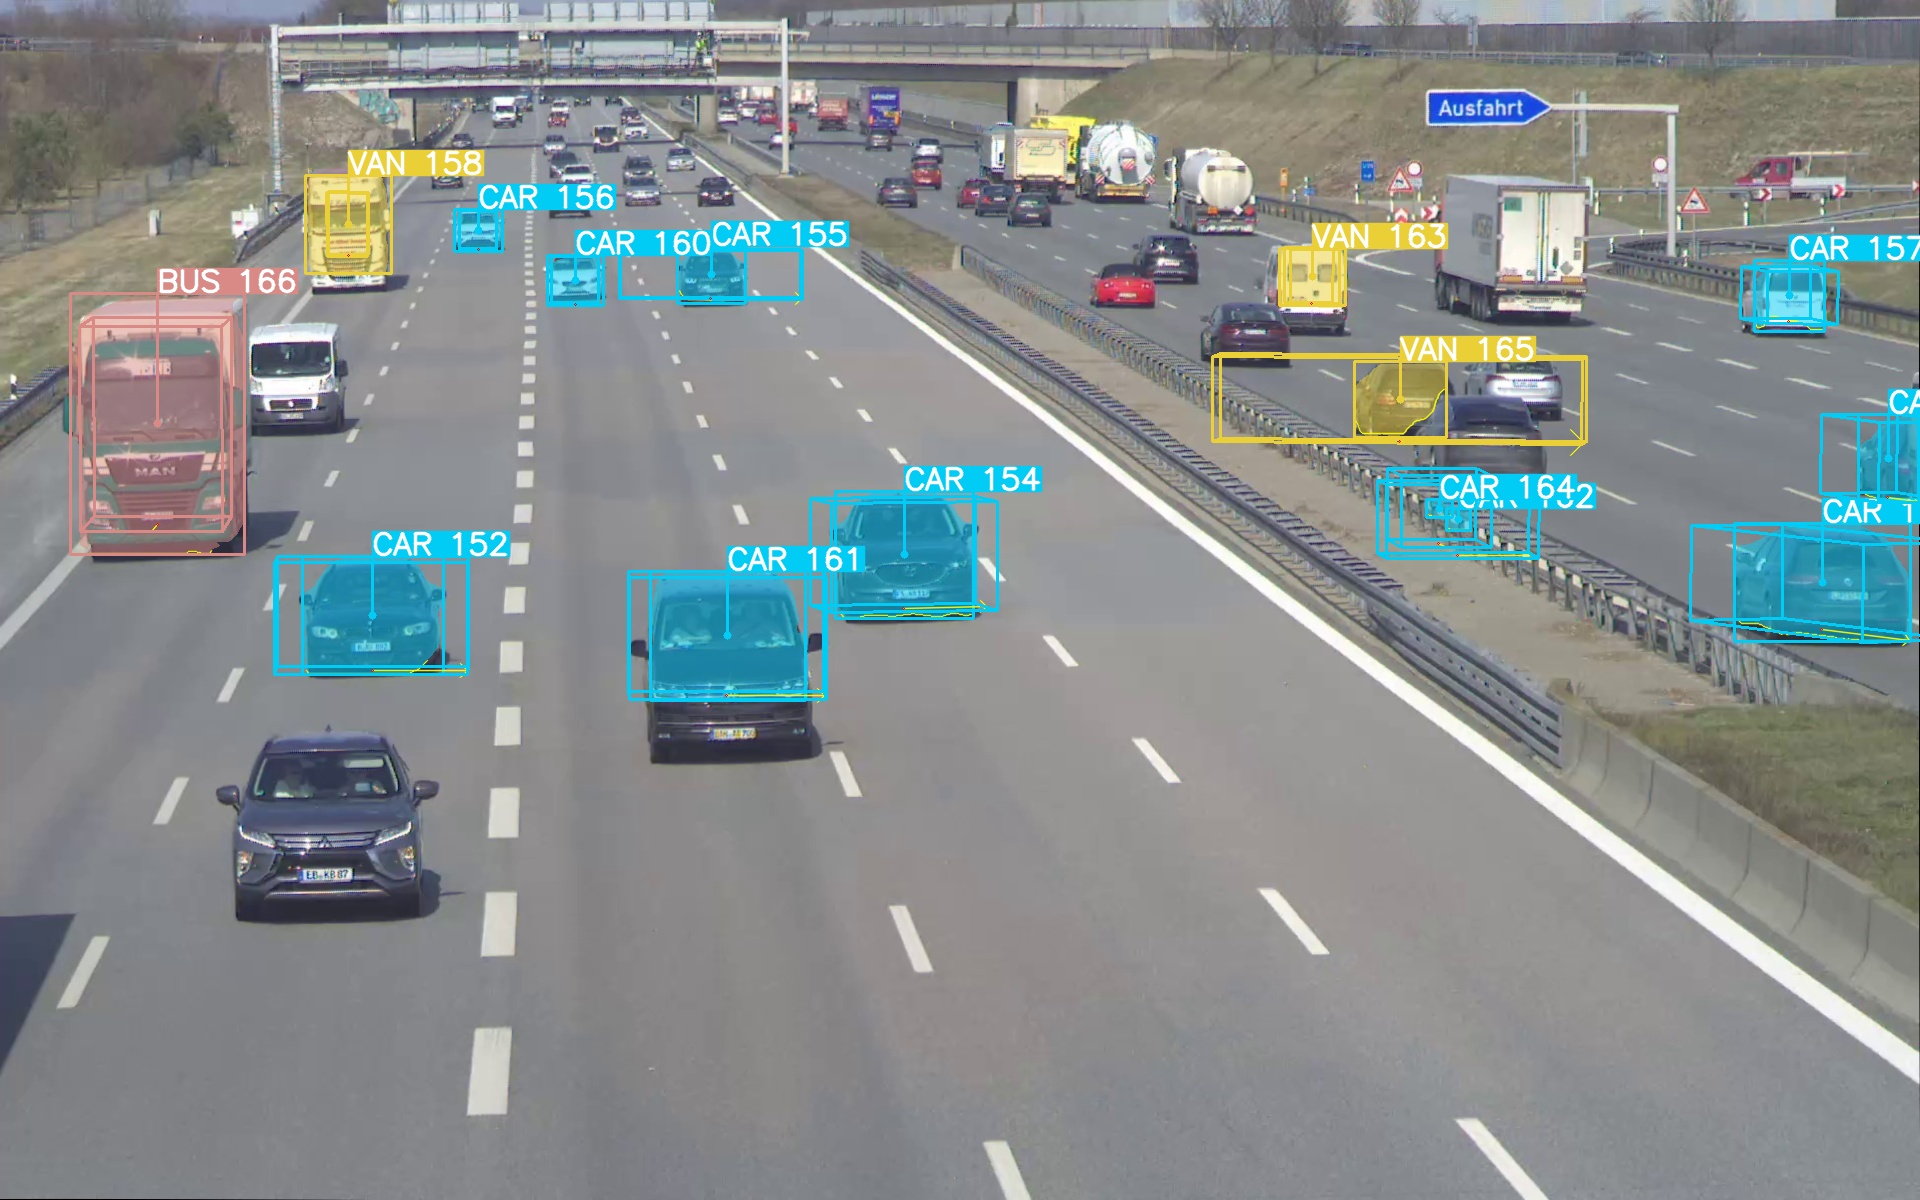
\includegraphics[width=\linewidth]{1616762525_089000000_finetuned.jpg}
		\end{subfigure}\hfill
		\begin{subfigure}{0.32\textwidth}
			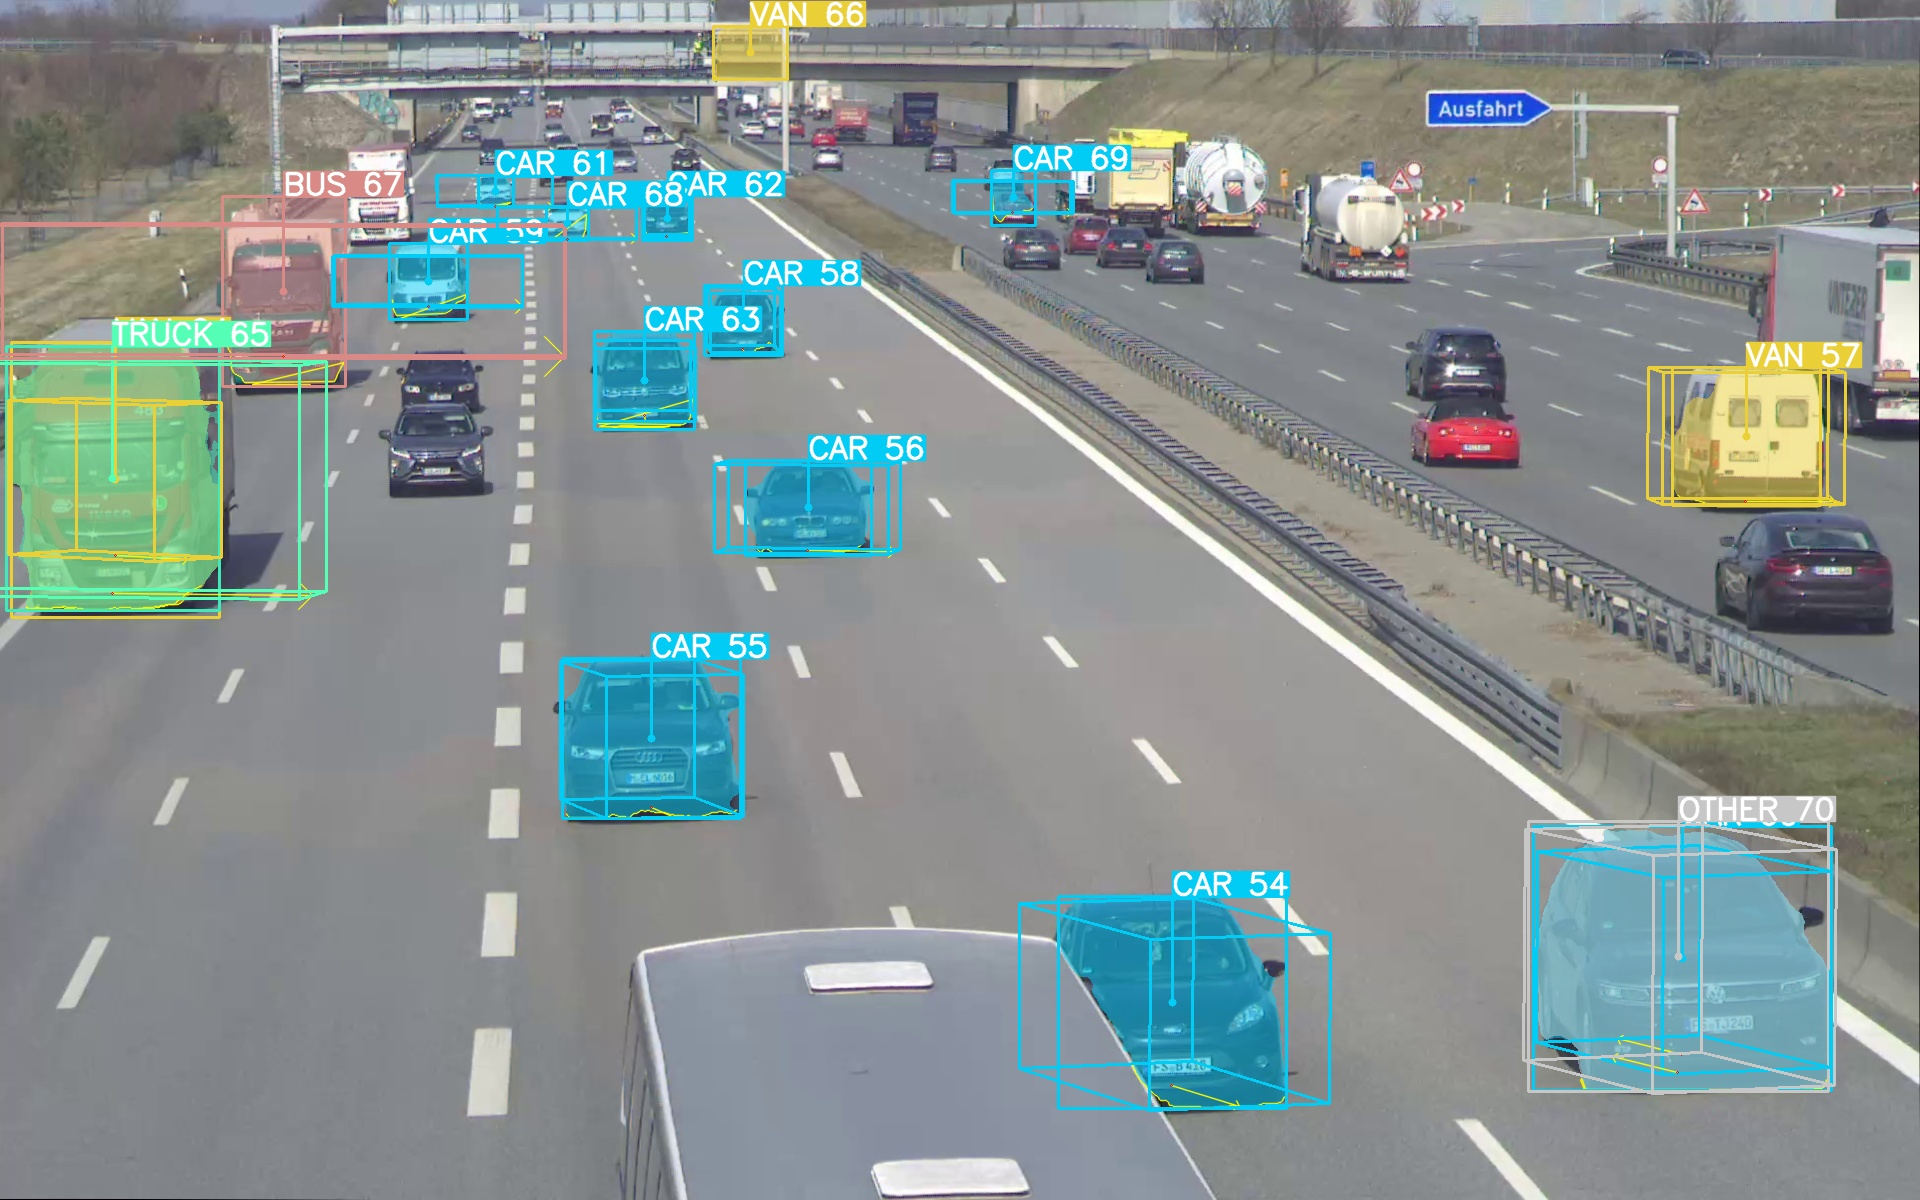
\includegraphics[width=\linewidth]{1616762522_288000000_finetuned.jpg}
		\end{subfigure}
		%\caption{\small $YOLOv8x\_coco\_tumtraf\_1920$}
	\end{subfigure}
	\captionof{figure}{ \textbf{Highway}: Qualitative comparisons on one high way sequence. Baseline detector YOLOv7\_coco (first row) and the proposed detector with model weight YOLOv8\_coco (second row), YOLOv8x\_tumtraf (third row) and with model weight YOLOv8x\_coco\_tumtraf\_1920 (fourth row).The visualizations include 2D bounding boxes, 2D masks, 3D bounding boxes, and category labels.}
	\label{figure:ablation_study_highway}
	\vspace{1em} 
\end{table}

\Cref{sec:ablation_study_highway} illustrates the inference results of different YOLO models on one frame sequence taken from the measurement station S40 on the A9 highway. Comparing the two model weights trained on COCO, YOLOv8x \_coco again outperforms YOLOv7\_coco. Interestingly, YOLOv8x\_coco can even identify humans sitting inside the vehicles. Overall, YOLOv8x\_coco also outperforms the other two models, YOLOv8x \_coco\_tumtraf\_1920 and YOLOv8x\_tumtraf on the highway, by detecting the most objects. 

In this scenario, the models fine-tuned on TUMTraf Intersection Dataset do not perform well. Compared to YOLOv8x\_coco, the YOLOv8x\_tumtraf model weight, trained solely on TUMTraf Intersection Dataset, can detect slightly less objects, especially the small vehicles much further away from the camera. 

Additionally, sometimes the detected mask is too large, as for the yellow van on the right of the first frame and the truck on the top left of the third frame. Occasionally, two adjacent large objects are also identified as a single object mask, such as the detected "TRUCK 103" in the top left corner of the fourth image. YOLOv8x\_coco\_tumtraf\_1920 performs poorly in this scenario with too few detections. 

This confirms that training and fine-tuning on TUMTraf Intersection Dataset will lead to performance boost in intersection scenarios but will not generalize well to other scenarios like highways. Therefore, to achieve the same performance boost as in intersection sequences, annotations for highway sequences also have to be extended with segmentation mask labels for training the models.

\section{Time-shifted ground truth labels and 3D tracker}

\begin{table}[htb]%
	\centering
	\begin{tabular}[htb]{lrrrr}
		\toprule
		\textbf{Model + Time-shifted} & \textbf{mAP@[.10]} & \textbf{$\triangle$ non Time-shifted}& \textbf{$\triangle$ Baseline} \\
		\midrule
		$YOLOv7\_coco$ (Baseline) & 15.20 & \textcolor{darkgreen}{+ 4.22} & \\
		$YOLOv8x\_coco$ & 17.77 & \textcolor{darkgreen}{+ 5.17} & \textcolor{darkgreen}{+ 2.57}  \\
		$YOLOv8x\_tumtraf$ & \underline{\textbf{33.31}} & \textcolor{darkgreen}{+ 14.80} & \textcolor{darkgreen}{+ 18.11}\\
		$YOLOv8x\_coco\_tumtraf\_1920$ & \textbf{22.26} & \textcolor{darkgreen}{+ 5.40} & \textcolor{darkgreen}{+ 7.06}\\
		\midrule
	\end{tabular}
	\caption{\textbf{Shifted ground truth}: 3D detection quantitative comparisons on the test sequence of TUMTraf Intersection Dataset from both camera south1 and camera south2 with time-shifted ground truth labels. $\triangle$non-shifted column shows the improvement achieved by using time-shifted ground truth compared to non time-shifted. $\triangle$baseline shows the improvement against the baseline model YOLOv7\_coco with time-shifted ground truth.}
	\label{tab:shifted_labels}
\end{table}

The TUMTraf Dataset provides 3D LiDAR labels. These labels, however, might be slightly shifted because of sensor delay between the RGB camera and the LiDAR sensor frame. The LiDAR label shifting technique, described in \cite{thesisJoseph}, involves estimating spatial velocity to correct label positions based on the known synchronization error time delta. \Cref{tab:shifted_labels} shows the quantitative evaluation after correcting the 3D LiDAR labels. These time-shifted LiDAR labels lead to an improvement in the overall performance compared to using original LiDAR labels. This enhancement demonstrates the importance of addressing sensor delay between the camera and LiDAR sensor frames, as it helps mitigate inherent inaccuracies in the LiDAR labels, ultimately enhancing evaluation accuracy.

\begin{table}[htb]%
	\centering
	\begin{tabular}[htb]{lrrrr}
		\toprule
		\textbf{Model + Time-shifted + polyMOT tracker} & \textbf{mAP@[.10]} & \textbf{$\triangle$ no tracker}& \textbf{$\triangle$Baseline} \\
		\midrule
		$YOLOv7\_coco$ (Baseline) & 16.23 & \textcolor{darkgreen}{+ 1.03} & \\
		$YOLOv8x\_coco$& 18.24 & \textcolor{darkgreen}{+ 0.47} & \textcolor{darkgreen}{+ 2.01}  \\
		$YOLOv8x\_tumtraf$ & \underline{\textbf{34.02}} & \textcolor{darkgreen}{+ 0.71} & \textcolor{darkgreen}{+ 17.79}\\
		$YOLOv8x\_coco\_tumtraf\_1920$ & \textbf{30.80} & \textcolor{darkgreen}{+ 8.54} & \textcolor{darkgreen}{+ 14.57}\\
		\midrule
	\end{tabular}
	\caption{\textbf{Shifted ground truth +  polymot 3D tracker}: 3D detection quantitative comparisons on the test sequence of TUMTraf Intersection Dataset from both camera south1 and camera south2 with time-shifted ground truth labels and 3D polyMOT tracker. $\triangle$no tracker column shows the improvement achieved by using 3D polyMOT tracker with time-shifted ground truth compared to only time-shifted ground truth. $\triangle$baseline shows the improvement against the baseline model YOLOv7\_coco with time-shifted ground truth labels and 3D polyMOT tracker.}
	\label{tab:polymot_3d_tracker}
\end{table}

\Cref{tab:shifted_labels} shows the additional quantitative improvement achieved when using a 3D tracker. The tracker employed in this study is Poly-MOT (a Polyhedral Framework for 3D Multi-Object Tracking) \cite{polymot}, which has been exploited and integrated into the toolchain as part of a bachelor thesis by Vitus Becker. Poly-MOT tracks detections in 3D space and enhances the stability of vehicle position estimates by continuously predicting and updating the status of objects within a video sequence. 

By using the Poly-MOT 3D tracker and evaluating against the time-shifted ground truth labels, the 3D mAP@[.10] can be further improved up to 15.51\%.%
% !TeX spellcheck = en_US
\chapter{Conclusion}  \label{chap:seven}%%

In conclusion, our thesis, conducted as part of the AUTOtech.agil project, has been dedicated to enhancing the 2D detector within the Providentia Mono3D object perception pipeline, with a focus on leveraging instance segmentation models to improve the system's final 3D perception performance, particularly on the TUM Traffic Intersection dataset.

Initially, we extend 1238 frames of the TUMTraf Intersection dataset with both modal and amodal instance masks to address the challenge of lacking segmentation annotations. Additionally, we present a simple approach for 2D annotation interpolation, utilizing algorithms like Jonker-Volgenant and linear interpolation to speed up the annotation process by at least five times.

Furthermore, our exploration into the state-of-the-art YOLOv8 segmentation model has yielded promising results. We extensively examine the effectiveness of pre-training on various datasets including COCO, KINS, and nuImages as well as fine-tuning on the annotated frames of the TUMTraf Intersection Dataset. Our experiments demonstrate the superiority of YOLOv8x pre-trained on COCO over the baseline YOLOv7 used in the Providentia live system, showing improvements of 3.6\% in 2D mAP@[.5:.95] and 1.53\% in 3D mAP@10. The fine-tuning of YOLOv8x on the TUMTraf Intersection dataset further improves performance, achieving a 10.5\% improvement in 2D mAP@[.5:.95] and 5.88\% in 3D mAP@10 compared to the baseline. Notably, this model excels in detecting large objects, addressing a significant limitation of the baseline YOLOv7 detector. The most significant performance boost, however, is achieved by the YOLOv8x model trained solely on the TUMTraf Intersection Dataset, with an 18.30\% improvement in 2D mAP@[.5:.95] and 7.53\% in 3D mAP@10 compared to the baseline. Together with the use of time-shifted ground truth labels and Poly-MOT 3D tracker, the best-trained model achieves a 3D mAP@10 of 34.02\% on the test sequence of the TUMTraf Intersection dataset, which is a 17.79\% improvement compared to the baseline YOLOv7 model trained on COCO. 

However, since all annotated frames come from the TUMTraf Intersection Dataset only, the trained models are overfitting on this intersection setting. This has been proven in our experiments on a highway sequence. 

In terms of speed, YOLOv8x exhibits accelerated inference speed. Once exported to TensorRT, this model achieves an inference speed of 200 FPS at a 640x640 resolution and 28 FPS at a 1920x1920 resolution, which is a 2.3 times speedup compared to the YOLOv7 model. This advancement allows for inference on full-resolution frames of 1920 while maintaining the system's real-time characteristics. The inference on full-resolution frames of 1920 has been shown to have 16.5\% higher 2D mAP@[.5:.95] than inference at 640 resolution. This highlights the significance of resolution in object detection accuracy, especially for small and far away object detection.

Additionally, we investigate the performance implications of segmenting full object masks instead of only visible ones using the amodal segmentation model C2F. Surprisingly, our experimental results indicate that utilizing amodal masks leads to a lower final 3D perception performance on the TUMTraf Intersection test set compared to solely relying on visible object masks detected by YOLOv8x. 


%
% !TeX spellcheck = en_US
\chapter{Outlook and Future Work}  \label{chap:eight}%%

In this chapter, we outline potential future work to address identified improvements from our implementation and evaluation process: 

\begin{itemize}
	\item As mentioned in \Cref{sec:2d_interpolation_pipeline}, the proposed 2D annotation interpolation pipeline utilizing the Jonker-Volgenant algorithm still sometimes generates erroneous object matching, requiring manual refinement afterward. Moreover, the currently used linear interpolation assumes a constant velocity of road users between frames. Future work could explore more advanced data association algorithms and leverage the existing Poly-MOT tracker to interpolate the 2D masks to more precise locations.
	
	\item Currently, only a limited number of frames, over one thousand, from the TUM Traffic Intersection dataset are annotated. While effective for training models specific to this intersection, this limited dataset poses a risk of overfitting. Consequently, models trained on this data exhibit improved performance at the intersection but suffer decreased performance on highway scenes compared to the baseline model YOLOv7. To address this limitation and train more generalized models, it is essential to annotate the remaining frames of the TUM Traffic Intersection Dataset and other releases of the TUM Traffic Dataset, such as the R00 and R01 release containing highway scenes and extended highway scenes in adverse weather conditions. The proposed 2D annotation interpolation pipeline can be refined and utilized for this task. 
	
	\item Another potential approach is to train separate models specifically tailored for intersection and highway scenes. By doing so, each model can be optimized for its respective environment, potentially leading to improved performance in both settings. Particular attention should be paid to overfitting prevention. The model can overfit quickly on the small amount of annotated frames. To prevent this, closely monitor the validation performance.
	
	\item The YOLOv8 model pre-trained on nuImages for 50 epochs is still not powerful enough to have any improvement over the model pre-trained on COCO. Given the vastness of the nuImages dataset and its potential benefits for model performance, our ongoing efforts involve continuing to pre-train the YOLOv8x segmentation model on nuImages. We are aiming for 200 epochs, and when the performance improves compared to pre-train on COCO, we will also fine-tune the model on the TUM Traffic Intersection dataset. 
	
	\item The trained YOLOv8 segmentation models can be exploited to run 2D multiple-object tracking. Ultralytics has implemented track algorithms, including BoT-SORT and ByteTrack, for the YOLOv8 model. The tracker produces the same output as segmentation, with an additional object ID that remains consistent for each object across consecutive frames. Therefore, after training a good and generalized model, future work can exploit 2D multiple-object tracking and investigate the performance of the two supported track algorithms. Exploiting a 2D multiple-object tracker with YOLOv8 is expected to enhance the overall performance by providing more stable predictions.
	
	\item As discussed in \Cref{sec:object_detection_with_yolov8}, transmitting segmentation instance masks in the form of polygon contours may offer greater efficiency compared to using bit-packed masks. Therefore, future work could adjust the 3D detector's message reception to accept polygon contours, eliminating the need to transmit bit-packed masks altogether.
	
	\item As revealed in \Cref{sec:quan_3d}, the 3D bounding box labels of the TUMTraf Intersection Dataset are incomplete, resulting in false positives during model evaluation. Future work should involve revising these labels, particularly for categories such as PEDESTRIAN, MOTORCYCLE, and BICYCLE, to ensure more accurate model evaluation and performance assessment.
	
	\item A YOLOv8 segmentation model trained on full-resolution frames can detect big objects successfully, however, with multiple overlapping masks. Future work can implement post-processing, which does not filter out the overlapping masks but merges them to receive one final mask with good coverage over the detected object. Objects from the frames taken at the intersection do not overlap much with each other. Therefore, an IoU threshold of around 0.6 to 0.7 can be used to decide if two masks are referring to the same object and should be merged. 
	
	\item Current evaluations of the C2F amodal segmentation model do not show improvement over only segmenting the visible part. The current C2F architecture crops frames based on each object's region of interest (ROI), resizes them to 256x256, extends them to amodal masks, and rescales them back to their original size within the original frame. However, as the system currently operates on the full resolution of 1920, 256x256 is relatively small, even for an object in the frame. This means that after upscaling a predicted amodal mask to its original size, the mask contour can be very unsmooth, which can affect the following bottom contour extraction step of the 2D-to-3D lifting stage of the system. In future work, the architecture of C2F can be adjusted to scale the ROIs to a bigger size.
	
\end{itemize}%
%
% Appendix
% --------
%\appendix%
%\chapter{Appendix 1}%
\Blindtext%
%
%
%
%
% References
% ----------
{%
    \sloppy% "Word"-like typesetting in order to improve breaking lines with long URLs/DOIs
    \printbibliography[heading=bibintoc]%
}%
%
%
\end{document}%
%
%
